\documentclass[draft=false
              ,paper=a4
              ,twoside=false
              ,fontsize=11pt
              ,headsepline
              ,BCOR10mm
              ,DIV11
              ]{scrbook}
\usepackage[ngerman,english]{babel}
%% see http://www.tex.ac.uk/cgi-bin/texfaq2html?label=uselmfonts
\usepackage[T1]{fontenc}
%\usepackage[utf8]{inputenc}
\usepackage[latin1]{inputenc}
\usepackage{libertine}
\usepackage{pifont}
\usepackage{microtype}
\usepackage{textcomp}
\usepackage[german,refpage]{nomencl}
\usepackage{setspace}
\usepackage{makeidx}
\usepackage{listings}
\usepackage{natbib}
\usepackage[ngerman,colorlinks=true]{hyperref}
\usepackage{soul}
\usepackage{hawstyle}
\usepackage{lipsum} %% for sample text
\usepackage{graphicx}

%% define some colors
\colorlet{BackgroundColor}{gray!20}
\colorlet{KeywordColor}{blue}
\colorlet{CommentColor}{black!60}
%% for tables
\colorlet{HeadColor}{gray!60}
\colorlet{Color1}{blue!10}
\colorlet{Color2}{white}

%% configure colors
\HAWifprinter{
  \colorlet{BackgroundColor}{gray!20}
  \colorlet{KeywordColor}{black}
  \colorlet{CommentColor}{gray}
  % for tables
  \colorlet{HeadColor}{gray!60}
  \colorlet{Color1}{gray!40}
  \colorlet{Color2}{white}
}{}
\lstset{%
  numbers=left,
  numberstyle=\tiny,
  stepnumber=1,
  numbersep=5pt,
  basicstyle=\ttfamily\small,
  keywordstyle=\color{KeywordColor}\bfseries,
  identifierstyle=\color{black},
  commentstyle=\color{CommentColor},
  backgroundcolor=\color{BackgroundColor},
  captionpos=b,
  fontadjust=true
}
\lstset{escapeinside={(*@}{@*)}, % used to enter latex code inside listings
        morekeywords={uint32_t, int32_t}
}
\ifpdfoutput{
  \hypersetup{bookmarksopen=false,bookmarksnumbered,linktocpage}
}{}

%% more fancy C++
\DeclareRobustCommand{\cxx}{C\raisebox{0.25ex}{{\scriptsize +\kern-0.25ex +}}}

\clubpenalty=10000
\widowpenalty=10000
\displaywidowpenalty=10000

% unknown hyphenations
\hyphenation{
}

%% recalculate text area
\typearea[current]{last}

\makeindex
\makenomenclature

\begin{document}
\selectlanguage{ngerman}

%%%%%
%% customize (see readme.pdf for supported values)
\HAWThesisProperties{Author={Nikolay Nikolaev Ishpekov}
                    ,Title={Cross-Plattform-Entwicklung von mobilen Enterprise-Anwendungen}
                    ,EnglishTitle={Cross-plattform-development of mobile enterprise Applications}
                    ,ThesisType={Bachelorarbeit}
                    ,ExaminationType={Bachelorpr�fung}
                    ,DegreeProgramme={Bachelor of Science Angewandte Informatik}
                    ,ThesisExperts={Prof. Dr. Olaf Zukunft \and Prof. Dr. Stefan Sarstedt}
                    ,ReleaseDate={18. Dezember 2015}
                  }

%% title
\frontmatter

%% output title page
\maketitle

\onehalfspacing

%% add abstract pages
%% note: this is one command on multiple lines
\HAWAbstractPage
%% German abstract
{Xamarin, Cross Plattform, App Entwicklung, Enterprise Apps, Business Apps, Applikationen}%
{In dieser Arbeit wird eine Alternative der herk�mmlichen Entwicklung von mobilen
Enterprise-Anwendungen (Enterprise-Apps), n�mlich Cross-Plattform-Appentwicklung vorgestellt.
Apps dieser Kategorie werden f�r die Optimierung von Gesch�ftsprozessen eingesetzt und zeichnen sich
dadurch aus, dass bei denen die Funktionalit�t h�chste Priorit�t hat. Visuelle
Effekten der Benutzungsoberfl�che werden selten bei solchen Apps angestrebt. Im
Rahmen dieser Arbeit wird das Cross-Plattform-Entwicklungsframework Xamarin evaluiert. Die Evaluierung erfolgt
anhand der plattform�bergreifenden Entwicklung einer Enterprise-App.}
%% English abstract
{Xamarin, cross platform, app development, business apps, enterprise apps, applications}%
{An alternative to the conventional
development of mobile enterprise applications (enterprise apps), namely cross platform
app development is presented in this work. Apps in this category are used for the optimization of
business processes and are distinguished by the fact that functionality has highest priority. The design of visual effects of
the user interface is rarely sought in such apps. The cross platform development framework Xamarin
will be evaluated in this bachelor thesis.
The evaluation is based on the cross platform development of an enterprise app.}

\newpage
\singlespacing

\tableofcontents
\newpage
% enable if these lists should be shown on their own page
\listoftables
\listoffigures
\lstlistoflistings

%% main
\mainmatter
\onehalfspacing
%% write to the log/stdout
\typeout{===== File: chapter 1}
%% include chapter file (chapter1.tex)
%%\include{chapter1}

%%%%
%% add some text to generate a sample document
%%\chapter{Sample Chapter}
\chapter{Einleitung}
\section{Motivation / Problembeschreibung}
Apps (mobile Softwareanwendungen) bekommen  eine immer gr��ere Bedeutung in der
heutigen Welt. Laut dem Bundesverband Informationswirtschaft, Telekomunikation und neue Medien
(BITKOM) nutzen 44 Millionen Deutsche ein Smartphone. Die Zahl der Smartphone-Nutzer ist in den letzten sechs Monaten
um rund 2 Millionen gestiegen. 74 Prozent der Benutzer laden zus�tzliche Apps auf ihr Ger�t
herunter. 
\\"`Das Smartphone ist zum digitalen Allesk�nner im Alltag avanciert und ersetzt dabei eine Vielzahl
von Ger�ten, die zuvor notwendig waren, wie zum Beispiel die Digicam oder den Wecker"',
sagt Johannes Weicksel von BITKOM \cite{BIT}.\\Die meisten Apps adressieren den Nutzer als
Konsumenten, aber in diesem Bereich liegen viele weitere M�glichkeiten.
Mit Business Apps k�nnen Unternehmen schnell und unkompliziert ihre
Gesch�ftsprozesse mobilisieren. Mobile Endger�te werden leistungsf�higer und es wird
eine Tendenz zur Nutzung von mobilen Ger�ten im Arbeitsleben beobachtet.
Durch diesen grundlegenden Wandel spielen Google, Facebook und Apple heutzutage eine gr��ere
Rolle als Nokia oder Siemens Mobile. \\Smartphones er�ffnen beinahe unbegrenzte M�glichkeiten, die
die Gesch�ftsprozessen in allen Branchen optimieren. 
Gesch�ftsabl�ufe werden automatisiert und Kundenkontakte finden situations- und ortsunabh�ngiger
statt. Heutzutage sind Smartphones und Tablet-PCs leistungsf�higer und mit mehr Funktionen ausgestattet als die Notebooks vor zehn
Jahren. Mit dem Einsatz von vielf�ltigen, mobilen Endger�ten wird ein Informationsfluss sowohl von
Kunden als auch von Gesch�ftspartnern direkt in die eigenen IT-Systeme erm�glicht.
\cite[4]{SmMApps}.

F�r die Erzeugung von Business Apps m�ssen
Softwarehersteller einige technische Barrieren �berwinden. Wahrscheinlich das gr��te Hindernis ist
die Heterogenit�t der mobilen Plattformen. Derzeit existieren mehrere mobile Betriebssysteme
(Siehe Abb.\ref{fig:abb1}) \cite{SmOSMaQ1}.
%%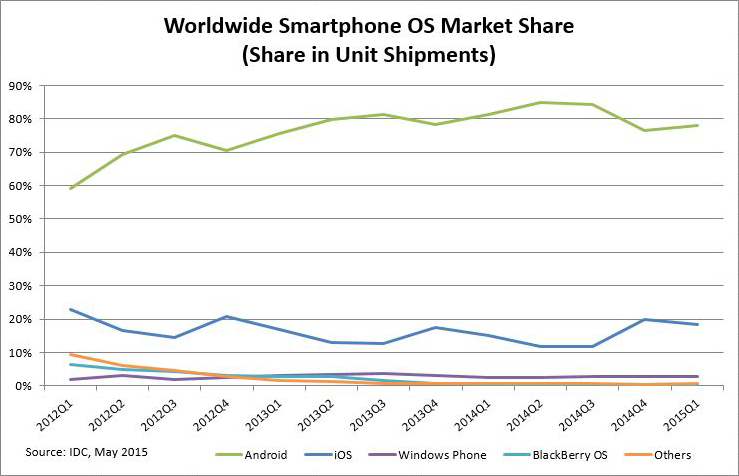
\includegraphics[scale = 0.7]{graphics/chartMSOSQ1.png} 
\begin{figure}[!h]
\centering
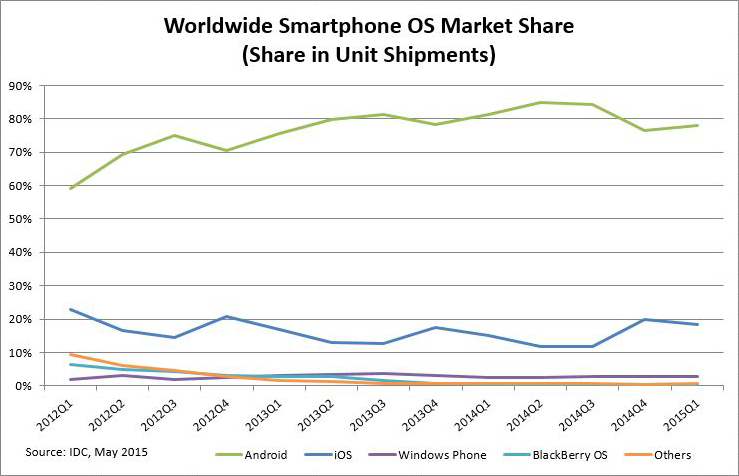
\includegraphics[scale = 0.7]{graphics/chartMSOSQ1.png}
\caption{Worldwide Smartphone OS Market Share}
\label{fig:abb1}
\end{figure}
\\In der Regel ist f�r jedes Betriebssystem eine eigene Management- und
Entwicklungsinfrastruktur n�tig und das ist mit hohen Kosten und langen Entwicklungszeiten
verbunden. Gesch�ftsanwendungen, die f�r eine nicht �berschaubare Anzahl von Nutzern bestimmt sind
und mit vielen Varianten ausgerollt werden, bringen ein Skalierbarkeit Problem mit. Wie k�nnen
Tausende von Endger�ten mit neuen Versionen einer Software betankt werden und wie kann im
Einzelnen sichergestellt werden, dass die neue Softwareversion sich mit dem Betriebssystem des
Endger�tes vertr�gt?\\Eine der h�ufigsten Anforderungen f�r eine Business Anwendung ist, dass die
App auf mehreren Mobilplattformen l�uft.
Da auf den meisten Smartphones entweder Android oder iOS installiert ist, spielen diese beiden
Plattformen eine zentrale Rolle f�r die Entwicklung von mobilen Softwareanwendungen.
Ungl�cklicherweise sind Android und iOS inkompatibel zueinander. Das bedeutet, dass ein Entwickler,
der eine auf beiden Plattformen lauff�hige App entwickeln m�chte, gezwungen ist, mehrere
plattformspezifischen Sprachen zu beherrschen.
 Man braucht Java, wenn man f�r Android entwickeln m�chte und Objective-C f�r iOS Anwendungen.
 Auch Windows Phone wird als Zielplattform immer attraktiver und das bedeutet einen gro�en
 Aufwand. Man muss quasi drei mal dieselbe Anwendung in drei verschiedenen Programmiersprachen
 implementieren. Aus gleichen Anforderungen resultieren drei v�llig unabh�ngige und unterschiedliche
  L�sungen.
\section{L�sungsidee}
 \textbf{Cross-Plattform-Entwicklung} k�nnte hier Abhilfe schaffen. Die Idee ist, dass man anstatt
  300 Stunden, nur 150 - 200 Stunden f�r die Entwicklung der App einplanen muss. Also
  Softwarehersteller k�nnen somit die Entwicklungskosten deutlich reduzieren. Dar�ber hinaus hat sich der
  Smartphonemarkt als unbest�ndig erwiesen und plattformgebundene App Entwicklung ist demzufolge ein riskantes
  Unterfangen. 
  
  Cross-Plattform-Technologien scheinen die Zukunft der App Entwicklung zu sein. Allerdings ist es
  keine einfache Aufgabe, eine geeignete plattform�bergreifenden Technologie auszuw�hlen. Diese
  Technologien sind relativ neu und es fehlt immer noch einen umfassenden �berblick �ber die Funktions- und Leistungsf�higkeit eines solchen Produktes. Die vorliegende
  Arbeit befasst sich mit der Untersuchung und Evaluierung einer solchen
  Cross-Plattform-Technologie, n�mlich Xamarin. Es wird eine praxisnahe Evaluation, anhand eines
  Fallbeispiels, durchgef�hrt. Dabei wird dargelegt, wie Xamarin als Cross-Plattform verwendet
  werden kann, um native Anwendungen f�r Android und iOS zu erstellen. Lohnt es sich f�r Softwarehersteller in Xamarin zu investieren? Ist Xamarin f�r
 Business Apps geeignet und welche Vor- und Nachteile bringt Xamarin mit? Es wird eine App
 nachgebaut, die schon f�r iOS und Android entwickelt wurde. Dabei ist interessant herauszufinden, an welchen Stellen es Probleme entstehen k�nnen und ob es �berhaupt m�glich ist,
  die App mit Xamarin zu entwickeln, so dass es keine Leistungsverluste gibt. Die ben�tigten
  Installationsschritte, sowie Hardware- und Softwarevoraussetzungen werden erl�utert. 

\section{Aufgaben und Ziele / Bewertungskriterien}
Ziel der Arbeit - eine Cross-Plattform-Entwicklungsumgebung zu evaluieren f�r die Entwicklung von
mobilen Enterprise-Anwendungen f�r heterogene Plattformen. (Anforderungen und Bewertungskriterien
stichpunktartig festlegen)



\chapter{Grundlagen der mobilen App Entwicklung}
Die App-Branche boomt. Von der hochspezialisierten
Business-App bis hin zu Game-Apps. Kaum ein Unternehmen kommt daran vorbei, eine oder mehrere Apps
anzubieten. Apps sind heutzutage zu einer Selbstverst�ndlichkeit geworden. Aber wie wird eine mobile
Anwendung erstellt? In diesem Kapitel werden die f�r das Verst�ndnis notwendigen Grundlagen der App Entwicklung erl�utert.
Die Themen werden stark komprimiert und vereinfacht vorgestellt.
\section{Aktuelle mobile Plattformen}
Mobile Betriebssysteme sind fest an ein bestimmtes Smartphone gebunden. Es ist nicht m�glich
fehlende Funktionen durch einen Betriebssystemwechsel zu erlangen.
Die Kombination aus Smartphone und Betriebssystem kann als feste Einheit betrachtet werden.
In K�rze werden die aktuellsten mobilen Betriebssystemen vorgestellt.
\begin{itemize}
  \item \textbf{Android}\\Das von Google entwickelte, mobiles Betriebssystem Android wurde im
  November 2007 der �ffentlichkeit vorgestellt. Es besteht aus einem Betriebssystemkern, Middleware
  und eigenen Applikationen (Telefonbuch, Kalender etc.). Da wesentliche Teile der Android Plattform unter einer Open Source Lizenz (Apache v2.0) stehen, kann Android von
  Lizenznehmern ohne Zahlung von Lizenzgeb�hren lizenziert und wegen der quelloffenen Verf�gbarkeit
  nach eigenen Bed�rfnissen angepasst werden. Neben der Bereitstellung von Programmierschnittstellen
  bietet Android auch umfassende Quellcodesammlung f�r Entwickler an. Der ebenfalls quelloffene
  Betriebssystemkern von Android basiert auf Linux 2.6.
  �ber "`Play Store"' (ein zentrales Softwareverzeichnis) lassen sich Applikationen kaufen und auf
  dem Ger�t installieren. Google �bernimmt f�r den Softwareentwickler die Distribution der Software und sorgt f�r eine kostenlose
  Verteilung von Updates. Das Inkasso erfolgt durch ein Zahlsystem von Google, wobei Google 30\% als
  Provision beh�lt und dem Entwickler monatlich 70\% des
  Verkaufserl�ses als Tantieme �berweist. Die Registrierung f�r den Android Market kostet einmalig
  \$25.
  Software kann alternativ auch direkt auf ein Ger�t mit Android installiert werden. Das
  Betriebssystem bringt Programme zum Senden und Empfangen von E-Mails, SMS, MMS, zum Aufnehmen und
  Abspielen von Fotos und Videos mit. Der Funktionsumfang beinhaltet auch ein Browser zum Surfen im
  Internet.
  \item \textbf{iOS}\\Das mobile Betriebssystem von Apple basiert auf der Grundlage des
  Betriebssystems Mac OS X und wurde zusammen mit dem iPhone im Juni 2007 eingef�hrt. Da Apple iOS
  nicht an andere Ger�tehersteller lizenziert, ist die Installation von iOS nur auf Apple-Ger�te
  m�glich. Das iOS-SDK, welches zum Entwickeln von iOS-Applikationen dient, setzt Apple Rechner mit
  Intel-Prozessoren voraus und alte Macs mit PowerPC-CPUs k�nnen nicht zum Entwickeln verwendet
  werden.
  Im Laufe der Zeit wurde das Betriebssystem und der damit verbundene
  Funktionsumfang sukzessive dem technologischen Fortschritt angepasst und beinhaltet einen
  E-Mail-Client, ein Programm zur SMS-Verwaltung, eine M�glichkeit, kabellos zu drucken, einen
  Browser, ein Tool zur Sprachsteuerung sowie eine Multimediaanwendung, um Videos und Bilder sowohl
  selbst zu erstellen als auch abzuspielen. Applikationen lassen sich nur durch Download �ber ein
  zentrales Softwareverzeichnis von Apple ("`App Store"') auf einem Ger�t installieren. Da Apple
  durch Signaturmechanismen die Installation von unsignierten Applikationen nicht zul�sst, ist es nicht
  m�glich unter Umgehung des App Stores Programme auf das Ger�t zu installieren. �hnlich wie bei
  Android �bernimmt der App Store eine Marktplatz-, Distributions-, Wartungs- und Inkassofunktion.
  Eine auf dem Apple Ger�t installiere Software �berpr�ft in regelm��igen Abst�nden, ob Updates f�r
  die gekaufte Apps vorhanden sind und der Benutzer wird dementsprechend benachrichtigt. Wie
  bei Android beh�lt Apple eine Verkaufsprovision in H�he von 30\%. Ein Vorteil von iOS
  gegen�ber Android ist die nicht so gro�e Vielfalt in Bezug auf Displaygr��e. Diese durchg�ngige
  Standardisierung vereinfacht die Entwicklung, Wartung, Test und Weiterentwicklung von iOS Apps aus
  Sicht des Entwicklers. Zum Testen auf Endger�ten und f�r die Ver�ffentlichung von Apps im Apples
  App Store ist allerdings eine kostenpflichtige Mitgliedschaft im iOS Developer Program
  erforderlich. Die Ger�te m�ssen im iPhone Developer Program unter DEVICES/ADD DEVICES hinzugef�gt
  werden.
  \item \textbf{Windows Phone}\\Microsoft bietet mit Windows Phone ein B�ndel aus Betriebssystem und
  einigen Zusatzprogrammen (Outlook, Word mobile etc.) f�r Smartphones. Windows Phone ist die
  Weiterentwicklung von Windows Mobile. W�hrend Windows Mobile einseitig an Business-Kunden
  ausgerichtet war, hat Windows Phone Gesch�fts- wie Consumer-Kunden im Auge. Im Gegensatz zu
  Microsoft Windows f�r station�re Desktop-PCs, das nahezu ausschlie�lich auf Intel-x86-Prozessoren l�uft, ist Windows Phone auf vielen unterschiedlichen Prozessorarchitekturen lauff�hig. Mit Windows Phone bietet Microsoft ein Betriebssystem mit einer akzeptablen Systemleistung trotz der oft begrenzten
  Hardwareressourcen von mobilen und embedded Ger�ten. Seit dem Erscheinen des Betriebssystem
  Windows Phone setzt Microsoft ein Kachelkonzept. Neben Funktionalit�ten wie SMS-Verwaltung,
  Telefonfunktion, Kalender und soziale Netzwerke, arbeitet Windows Phone nach dem Prinzip des
  Cloud-Computing. Bspw. Dienste wie Facebook werden integriert und mit den Funktionen des
  Betriebssystems verkn�pft. Damit Apps auf einem Windows Phone Ger�t installiert und getestet
  werden k�nnen, muss das Ger�t explizit als Entwicklerger�t freigeschaltet werden. Dazu muss man sich
  zuerst bei Microsoft als Entwickler registrieren, was 99 EUR im Jahr kostet. Das ist auch
  notwendig, wenn man Apps im Microsoft Market (vergleichbar mit App Store und Play Store)
  ver�ffentlichen m�chte. \cite[17]{AppsPhoneGap}
  \item \textbf{Blackberry OS}\\Das Betriebssystem wird von Research In Motion (RIM)  f�r die
  Nutzung auf Smartphones des Typs Blackberry hergestellt. �hnlich wie bei iOS von Apple ist es nur
  f�r Blackberry-Smartphones vorgesehen. Da Blackberry-Smartphones vorwiegend auf
  Gesch�ftskunden ausgerichtet und bieten sie komfortable Synchronisationsmechanismen f�r Daten
  zwischen einem Server und dem Smartphone, sowie einen Push-Email Dienst an. Damit sich native Applikationen st�rungsfrei
  auf einem Blackberry-Smartphone installieren und ausf�hren lassen, m�ssen diese zuvor von RIM
  digital signiert werden.
\end{itemize}
\cite[347]{MoApp1}
\cite[98]{App4U}
\\Laut International Data Corporation (IDC) ist Android das am weitesten verbreitete mobiles
Betriebssystem mit einem Marktanteil von 78\%, es folgen iOS mit 18.3\%, Windows Phone mit 2.7\% und
Blackberry OS mit 0.3\%. Allerdings hat Android ca 3\% Marktanteil verloren im Vergleich zum Vorjahr
und iOS hat dagegen 3\% mehr (\cite{SmOSMaQ1}).\\Da Android und iOS einen enormen Vorsprung auf die
anderen mobilen Betriebssystemen haben, was die Verbreitung angeht, wird sich diese Arbeit stark auf diese zwei
Betriebssystemen konzentrieren.
\section{Mobile Applikationen}
\begin{quote} 
"`Eine \textbf{mobile Applikation} stellt eine spezifische Anwendungssoftware dar, die zur
Anwendung auf einem Betriebssystem sowie zur Ausf�hrung auf mobilen Endger�ten entwickelt wird
und neben der Ber�cksichtigung besonderer Endger�teeigenschaften, die Nutzung kabelloser
�bertragungstechniken voraussetzt."'\footnotemark[1]
\end{quote}
\footnotetext[1]{\cite[105]{App4U}}
Der Begriff Applikation (App) hat sich in Bezug auf die mobile Nutzung und
Anwendung als eigenst�ndiger Begriff etabliert. Eine App wird als nativ bezeichnet, wenn sie 
f�r eine bestimmte mobile Plattform entwickelt wurde und nur auf dieser Plattform installiert und
ausgef�hrt werden kann. Die Vorteile einer nativen App sind eine gute Performance und vor allen
Dingen die M�glichkeit zum Zugriff auf besondere Hardwarebestandteile der mobilen Endger�te.
Ebenso k�nnen viele vorgefertigte Features aus nativen Schnittstellen und APIs benutzt werden. Da
die verschiedenen Verzeichnisdienste, wie App Store, Play Store oder Microsoft Market, native Apps
einfordern, kommt man um eine echte Anwendung nicht herum, wenn man einen kommerziellen Vertrieb
einer App anstrebt.\\Informationssuche und Nachrichten�bermittlung stand anfangs im Fokus des
mobilen Internets.
Allerdings hat sich im Laufe der Zeit ein Bed�rfnis nach Interaktion und
Mitgestaltung entwickelt. Daraus resultiert die Nachfrage nach einfach zu bedienenden Ger�ten sowie
intuitiv steuerbare Applikationen. Immer mehr Unternehmen erkennen den daraus resultierenden
Mehrwert und erm�glichen den Zugriff auf Dienstleistungen �ber mobile Anwendungen. Es entstehen
Dienstleistungsangebote sowie im privaten als auch im gesch�ftlichen Bereich. Aus
produktorientierter Sichtweise lassen sich vier Klassen mobiler Anwendungen
identifizieren:\cite[102]{App4U}
\begin{itemize} 
  \item \textbf{Informationsorientierte} Dienste (z.B. Reiseinformationen, B�rseninformationen
  etc.)
  \item \textbf{Applikationsorientierte} Dienste (z.B. Computerspiele, �bersetzungsdienste etc.)
  \item \textbf{Transaktionsorientierte} Dienste (z.B. Bezahldienste, Reservierungsdienste etc.)
  \item \textbf{Kommunikationsorientierte} Dienste (z.B. E-Mail, Chat oder soziale Netzwerke)
\end{itemize}
Mobile Applikationen werden in drei unterschiedliche Komplexit�tsstufen eingeteilt:
 \begin{itemize}
   \item \textbf{Einfache Apps} zeichnen sich durch wenig Logik, keinen Backendzugriff,
   minimalistisches Design und die �berwiegende Verwendung von Standardkomponenten aus.
   \item \textbf{Durchschnittliche Apps} verwenden ebenfalls kein eigenes Backend, k�nnen aber auf fremde Backends zugreifen. Bei
durchschnittlichen Apps sind vereinzelte Konfigurationsm�glichkeiten und mehrere Bildschirme
m�glich.
   \item \textbf{Komplexe Apps}. F�r die Entwicklung einer komplexen mobilen Anwendung ist eine Konzeption und Umsetzung
eines eignen Backends notwendig. Dazu kommt noch die Einbindung von Men�s und umfangreicheren
Konfigurationsm�glichkeiten und Anpassung der Layouts nach eigenen W�nschen. Auch
Funktionen und Komponenten zum Datenschutz und zur Dienstsicherheit sollten eingebaut werden.
\end{itemize}
Laut einer Studie der Marktforscher des "`HighText Verlags"', die im Jahr 2013 ver�ffentlicht
wurde, fallen die Honorare bei der Entwicklung mobiler Anwendungen in Deutschland an (Siehe Tabelle
\ref{table1}). Die Entwicklungskosten f�r iOS und Android haben sich im Laufe der Zeit stark
angen�hert und f�r Nischenbetriebssysteme, wie z.B. das Betriebssystem Symbian von Nokia k�nnen die
Kosten bis zu 45\% h�her anfallen. Grunds�tzlich lassen sich zwei Berechnungsmodelle f�r die Preise
unterscheiden: der Pauschalpreis und der Preis pro Funktion, wobei ein Gro�teil der in Deutschland
entwickelten mobilen Anwendungen nach dem Preis pro Funktion kalkuliert wurde.
\begin{table}
\begin{tabular}{|l|l|l|l|l|}\hline
Komplexit�tsstufe & Jahr & Minimum\footnotemark[2] & Durchschnitt\footnotemark[2] &
Maximum\footnotemark[2] \\
\hline Einfache Anwendung & 2011  & 760  & 16500 & 97000 \\
Einfache Anwendung & 2013  & 601  & 7754 & 78790 \\ \hline
Durchschnittliche Anwendung & 2011  & 2450  & 23000 & 105000 \\
Durchschnittliche Anwendung & 2013  & 809  & 13397 & 65933 \\ \hline
Komplexe Anwendung & 2011  & 6000  & 79000 & 520000 \\
Komplexe Anwendung & 2013  & 802  & 48804 & 382215 \\ \hline
\hline
\end{tabular}
\caption{Durchschnittspreise f�r die mobile Anwendungsentwicklung in Deutschland.}
\label{table1}
\end{table}
\cite[31]{App4U}
\footnotetext[2]{Alle Preise sind in Euro}


\section{Software Architekturmuster f�r mobilen Anwendungen}
Ohne Frameworks und Debugging Tools w�re die Programmierung einer Applikation kaum vorstellbar.
Bei Frameworks handelt es sich um ein Programmierger�st zur Softwareentwicklung, das Entwicklern
vorgefertigte Designstrukturen und Codefragmente zur Verf�gung stellt. Debugging Tools werden w�hrend des
Entwicklungsprozesses, zur Fehlerentdeckung und Verbesserung des Programmcodes,
eingesetzt. Durch die Verwendung von Frameworks k�nnen Softwareentwickler auf entsprechende
Standardbausteine zugreifen, sodass nicht bei jedem neuen Entwicklungsprojekt das Rad neu erfunden
werden muss.\\Das Entwickeln der Benutzeroberfl�che (auf Englisch User Interface oder kurz UI) einer
professionellen Softwareanwendung ist nicht einfach. Es kann eine schwer durchschaubare Mischung aus
Daten, Interaktionsentwurf, visuellem Entwurf, Konnektivit�t, Multithreading, Sicherheit,
Internationalisierung, �berpr�fung, Komponententests und etc. sein. In Anbetracht der Tatsache, dass
eine Benutzeroberfl�che eng mit dem zugrunde liegenden System verbunden ist und die nicht immer
voraussagbaren stilistischen Anspr�che ihrer Benutzer entgegenkommen muss, kann dies der brisanteste Bereich vieler Anwendungen sein.
Hierf�r k�nnen Architekturmuster Abhilfe schaffen.
\cite[195]{App4U}
\subsection{Model-View-Controller (MVC)}
\begin{figure}[!h]
\centering
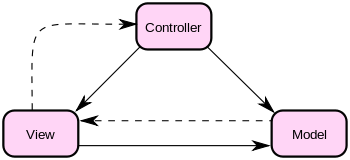
\includegraphics[scale = 0.5]{graphics/ModelViewControllerDiagram.png}
\caption{Model-View-Controller-Konzept. Die durchgezogene Linie symbolisiert eine direkte
Assoziation, die gestrichelte eine indirekte Assoziation (z.B. �ber einen Beobachter).Quelle:\cite{WikiMVCBild}}
\label{fig:abb8}
\end{figure}
Das \textbf{Model-View-Controller} (\textbf{MVC}) Muster (siehe Abb.\ref{fig:abb8}) gibt es schon
seit Jahrzehnten und wurde zusammen mit der Programmiersprache Smalltalk entwickelt. 
Man kann es sich vereinfacht folgenderma�en vorstellen:
\begin{itemize} 
  \item Die Daten, die auf dem Bildschirm angezeigt werden, sind das \textbf{Model}. Das Model
  enth�lt bis auf Such- und Sortierfunktionen keine Gesch�ftslogik. Diese Schicht kapselt die Daten
  der Anwendung in Klassen. Das Model besitzt also Klassen zur Speicherung und Verarbeitung von
  Daten und sorgt daf�r, dass die Daten konsistent gehalten werden. 
  \item Die \textbf{View}-Komponente ist f�r die Darstellung auf dem Bildschirm und das
  Verarbeiten von Benutzereingaben zust�ndig. Das sind also Klassen, die sowohl etwas anzeigen, als
  auch Klassen, die Benutzer-Eingaben verarbeiten k�nnen. Die View-Schicht darf den Zustand der
  Anwendung nur lesen.
  \item Der \textbf{Controller} verkn�pft Model und View. Er wertet die von der View
  entgegengenommenen Benutzereingaben aus und bekommt lesenden und schreibenden Zugriff auf das Model. Somit kann der
  Controller den Zustand der Anwendung ver�ndern. 
\end{itemize} 
Die Controller-Schicht enth�lt also die Gesch�ftslogik der Anwendung und �bernimmt die Steuerung des
Programms.
Weder das Model noch die View sollten die Klassen oder Methoden des Controllers kennen. Auf diese
Weise wird eine Wiederverwendbarkeit der Model- und View-Schichten erreicht. Jedes Model-Objekt kann
also durch unterschiedliche Controller verarbeitet und �ber verschiedene Views dargestellt werden
und jede View l�sst sich in vollkommen unterschiedliche Applikationen einsetzen.\cite{AppsForiPhone}
\subsection{Model-View-ViewModel (MVVM)}
\begin{figure}[!h]
\centering
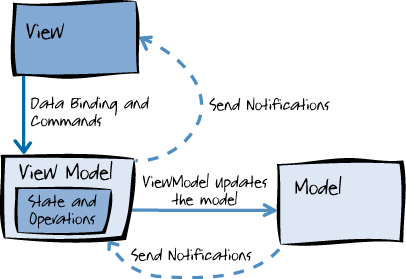
\includegraphics[scale = 0.7]{graphics/MVVMBild.png}
\caption{MVVM-Muster.Quelle:\cite{MSDNA2MVVM}}
\label{fig:abb9}
\end{figure}
Im Jahr 2005 stellte John Gossman, derzeit einer der Windows Presentation Foundation (WPF)- und
Silverlight-Architekten bei Microsoft, das \textbf{Model-View-ViewModel} (\textbf{MVVM})-Muster
(siehe Abb.\ref{fig:abb9}) in seinem Blog vor.
MVVM besteht aus drei Komponenten und ist MVC sehr �hnlich, der Unterschied ist, dass wir
hier anstatt Controller ein sogenanntes ViewModel haben und das Model im Gegensatz
zum Model von MVC nicht nur auf Such- und Sortierfunktionen begrenzt ist:
\begin{itemize} 
  \item \textbf{Model}. Das Model enth�lt die Gesch�ftslogik.
  \item \textbf{View}. Die View (Ansicht) repr�sentiert die Benutzerschnittstelle. Die Ansicht wird
  in einer deklarativen Programmiersprache, wie bspw. XAML, erstellt. Es ist lediglich eine reine
  Beschreibung der Ansicht und enth�lt keine Ausf�hrungslogik.
  \item \textbf{ViewModel}. Das ViewModel nimmt die Informationen vom Model und wandelt sie in eine
  von der View verwendbare Form um. Es nimmt au�erdem die �nderungen aus der View und ruft die entsprechende
  Funktionalit�t im Model auf. Es handelt sich also um eine Vermittlungsschicht zwischen dem Model
  un der View. 
\end{itemize} 
Es ist ein sehr lose gekoppelter Entwurf und dadurch wird das Unit-Testing erleichtert.
Das Muster weist eine Abstraktion einer Ansicht auf, die den Zustand und das Verhalten einer
Ansicht enth�lt. Diese Abstraktion einer Ansicht wird als ViewModel bezeichnet.\\Ein ViewModel ben�tigt
keinen Verweis auf eine View.
Die View wird an die Eigenschaften eines ViewModels gebunden, das wiederum Daten verf�gbar macht, die in Modellobjekten und anderen f�r diese Ansicht spezifischen
Zust�nden enthalten sind. Das Erstellen der Bindungen zwischen Ansicht und ViewModel ist einfach, da
ein ViewModel-Objekt als DataContext einer Ansicht festgelegt wird. Wenn sich Eigenschaftswerte im
ViewModel �ndern, werden diese neuen Werte automatisch �ber die Datenbindung an die Ansicht
weitergeleitet. Wenn der Benutzer auf eine Schaltfl�che in der Ansicht klickt, wird im ViewModel ein
Befehl ausgef�hrt, um die angeforderte Aktion durchzuf�hren. Das ViewModel, aber niemals die
Ansicht, f�hrt alle an den Modelldaten vorgenommenen �nderungen durch. Die View-Klassen wissen
nicht, dass die Modell-Klassen existieren, w�hrend dem ViewModel und dem Modell die Ansicht nicht
bekannt ist. Das Modell wei� nichts dar�ber, dass das ViewModel und die Ansicht existieren (siehe
Abb.\ref{fig:abb9}).
Durch das Binden von Eigenschaften einer View an ein ViewModel kommt es zur losen Kopplung zwischen den
beiden, wodurch in einem ViewModel kein Code geschrieben werden muss, der eine Ansicht direkt
aktualisiert.\\Ein besonderer Vorteil von MVVM ist die M�glichkeit, Komponententests an
ViewModel-Klassen durchzuf�hren.
\cite{MSDNAMVVM}
\section{Plattformspezifische Entwicklung (App Life-Cycle)}
Mit dem Begriff Software-Life-Cycle wird die Zeitspanne beschrieben, in der ein Softwareprodukt
geplant, entwickelt und bis zum Ende seiner Nutzung eingesetzt wird (siehe Abb. \ref{fig:abb5}).
Mobile Anwendungen werden als nativ bezeichnet wenn, die auf einem bestimmten Endger�tetyp und dessen zugeh�rigen Betriebssystem lauff�hig sind. Die Entwicklung nativer Apps ist dann sinnvoll,
wenn die Applikation auf gegebene Hardware- und Softwareressourcen eines bestimmten Endger�tes
zugreifen soll, bspw. auf die interne Kamera, Bewegungssensoren oder GPS. Android, iOS und Windows
Phone sind inkompatibel zueinander, da diese Plattforme unterschiedliche API-Befehle benutzen.\\Im
Folgenden wird die App Entwicklung f�r die g�ngigsten mobilen Betriebssysteme vorgestellt. 
\begin{figure}[!h]
\centering
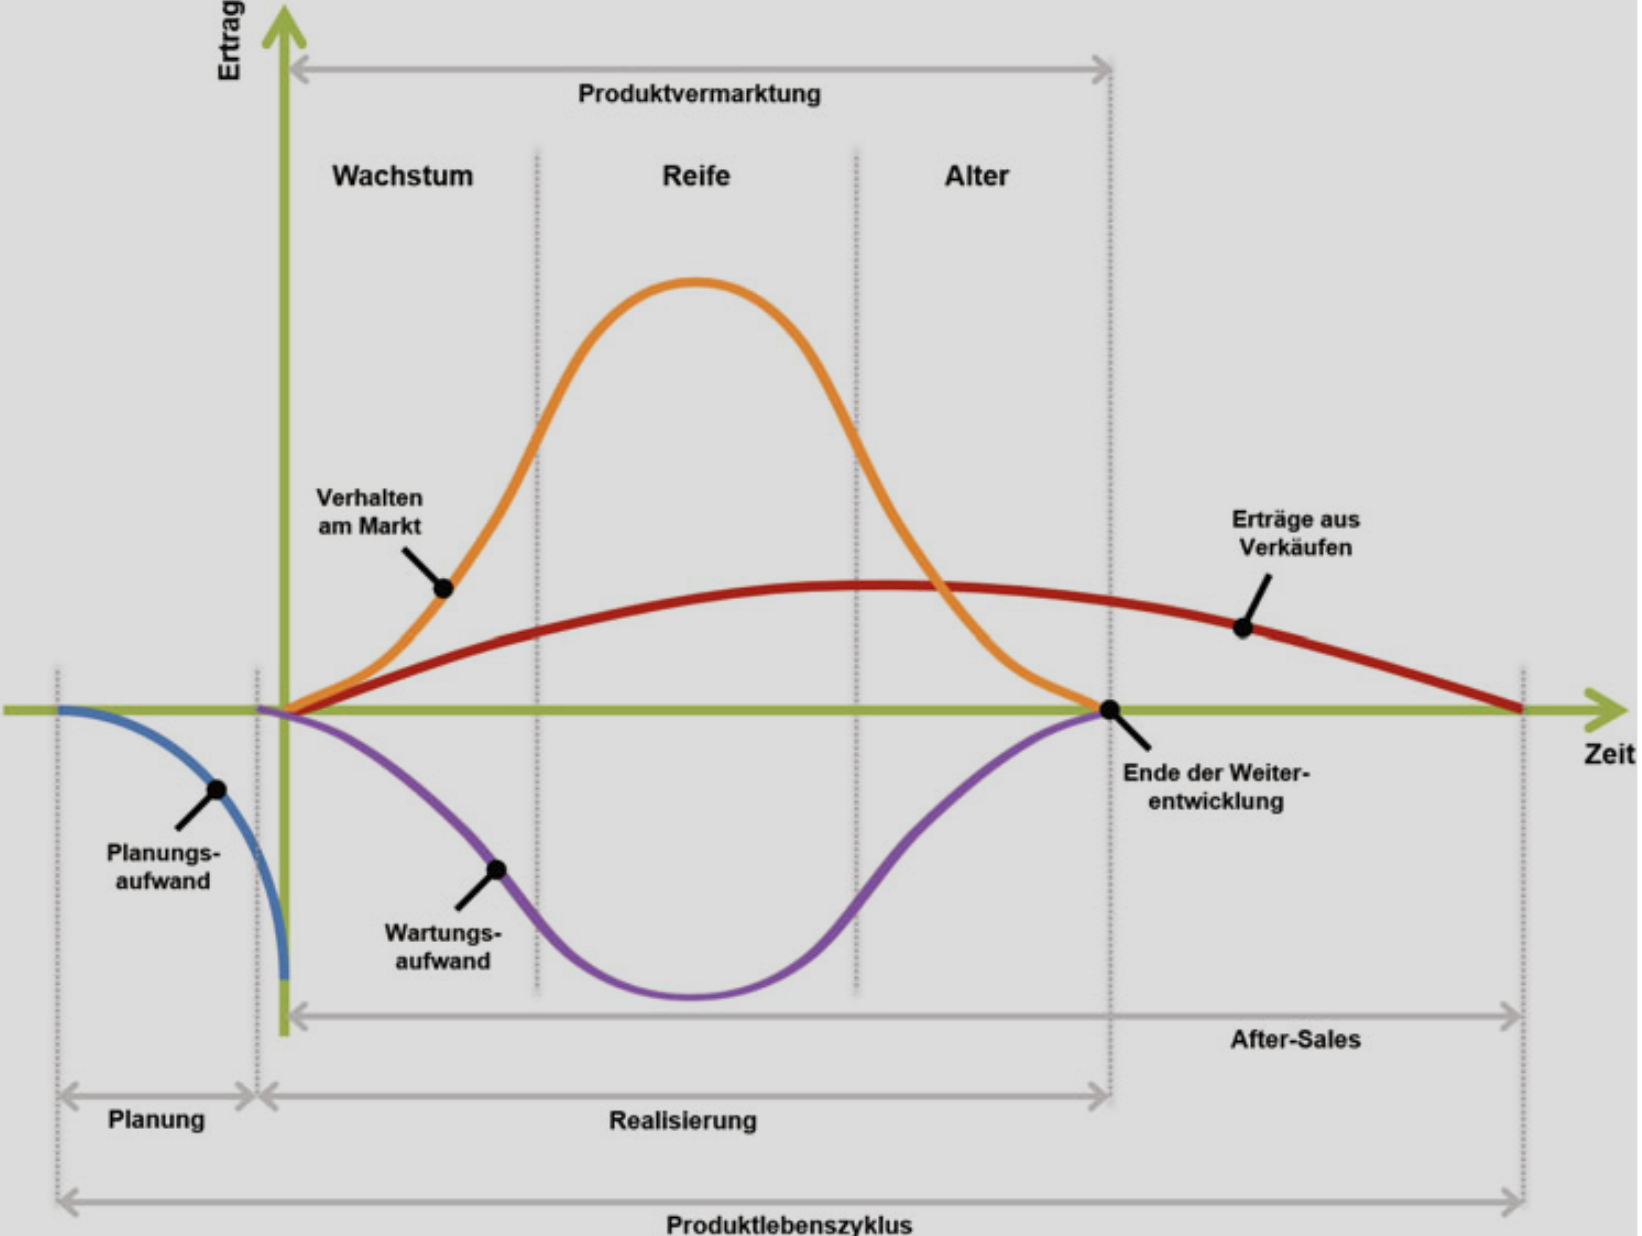
\includegraphics[scale = 0.5]{graphics/App_Lifecycle.png}
\caption{App Life-Cycle \cite[154]{App4U}}
\label{fig:abb5}
\end{figure}
\subsection{Android}
Android Apps werden mit der Programmiersprache Java programmiert. 
Als erstes muss man das
  Java Development Kit (JDK) installieren. Das JDK dient zum Kompilieren der
  Java-Textdateien in .class-Dateien. Man braucht noch das Android Software Development Kit (SDK).
  Im Gegensatz zu iOS Apps gibt es mehrere Entwicklungsumgebungen, mit denen man
Android Apps entwickeln kann. Die k�nnen auch auf allen Plattformen erstellt werden, auf denen
Java-Entwicklung m�glich ist. Die Entwicklungsumgebung Eclipse hat sich als Standard f�r
Android-Entwicklung etabliert. Eclipse ist unter der Open-Source-Lizenz frei verf�gbar und wurde
urspr�nglich als integrierte Entwicklungsumgebung f�r die Programmiersprache Java genutzt. Seit der Version 3.0
ist die Einbindung von Plug-ins zur Erweiterung des Funktionsumfangs m�glich und somit k�nnen
nahezu alle Programmiertechniken abgedeckt werden. Eclipse gibt es sowohl f�r Linux und Windows als
auch f�r Mac OS. Die Installation von Eclipse ist vollkommen unproblematisch, wenn auf einem Rechner
bereits ein JDK installiert ist. Eclipse wird als komprimierte Datei ausgeliefert, die einfach
extrahiert werden muss. Beim ersten Start such sich die IDE die passende Java-Umgebung und richtet
das System weitgehend automatisch ein.\\Um Android Apps mit Eclipse entwickeln zu k�nnen, muss das
Android-Developer-Tools Plug-in (ADT) eingebunden werden.
Im SDK-Manager k�nnen die verschiedenen Android-Versionen ausgew�hlt werden. Die API-Level von
Android sind abw�rtskompatibel, deswegen muss der Entwickler die niedrigste unterst�tzte Version
ausw�hlen. Zu empfehlen ist API-8 auszuw�hlen. Mit dem in dem ADT-Paket enthaltenen
Virtual-Device-Manager lassen sich virtuelle Android-Ger�te erstellen. Diese lassen sich mit
verschiedenen Android-Versionen, Displayaufl�sungen, internem Speicherplatz, Arbeitsspeicher und
vielem mehr konfigurieren. Auf diese Weise kann man das Testen der Anwendung auf verschiedenen
Ger�ten simulieren. Allerdings empfiehlt es sich, die Anwendung auf m�glichst vielen echten Ger�ten
zu testen.\\Um ein Smartphone oder Tablet mit Eclipse zu verbinden, m�ssen zun�chst die
Entwickleroptionen des Ger�ts aktiviert werden und anschlie�end es per
USB an den PC anschlie�en.\\Mit dem Android NDK (Nativ Development Kit) bietet Android die
M�glichkeit an, Teile der Applikation in nativen Programmiersprachen zu implementieren.
Die meisten Apps brauchen NDK nicht, aber f�r manche ist es hilfreich, C oder C++ Bibliotheken verwenden zu k�nnen.
\\Der Android-SDK kompiliert den Java-Code und packt das Programm und alle anderen zugeh�rigen Ressourcen, wie
Layoutdateien und Grafiken, in eine .apk-Datei.
\\\textbf{Dalvik} ist eine virtuelle Maschine, die JVM (Java Virtual Machine) �hnlich ist, aber
speziell an die Einschr�nkung mobiler Ger�te angepasst wurde. Der Java-Bytecode wird mit dem
Dalvik-Compiler zu Dalvik-Bytecode kompiliert und anschlie�end von der Dalvik-VM ausgef�hrt. Auf
diese Weise wird abgesichert, dass selbst wenn an der Sprache Java �nderungen vorgenommen werden,
der Java-Bytecode gleich bleibt (siehe Abb.\ref{fig:abb6}). Alle Kompilationsschritte werden von den
Entwicklungswerkzeugen automatisiert, so dass keine zus�tzlichen Arbeitsschritte f�r den Entwickler
anfallen. Jede Anwendung in Android wird in einer eigenen virtuellen Maschine, der sogenannten
Sandbox, ausgef�hrt. Jede Anwendung ist somit isoliert von den anderen Apps und kann nur auf ihre
eigene Daten zugreifen. So wird unter anderem bei einem Absturz die Stabilit�t des Systems
gew�hrleistet.
Die Entwicklung von Applikationen f�r Android erfolgt nach dem Model-View-Controller Architekturmuster. Im Folgenden werden die wichtigsten Komponenten einer Android Applikation vorgestellt.
\cite[317]{App4U}
\begin{figure}[!h]
\centering
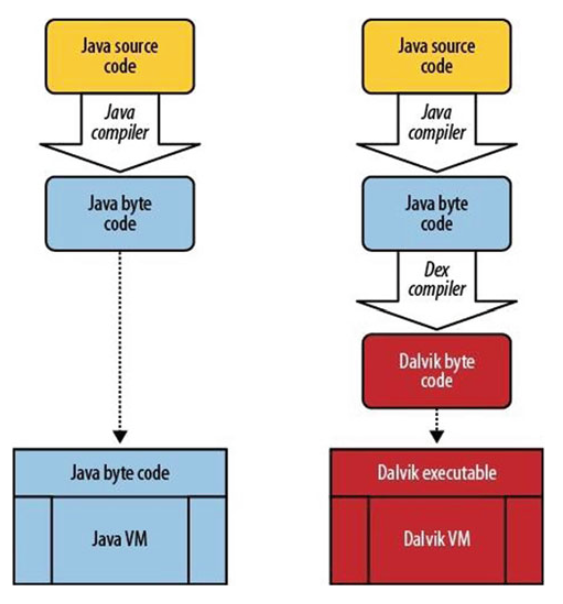
\includegraphics[scale = 0.5]{graphics/JVMvsDavlik.png}
\caption{Vergleich JVM und Dalvik-VM. \cite[318]{App4U}}
\label{fig:abb6}
\end{figure}
\subsubsection{AndroidManifest.xml}
Die wichtigste Datei in jeder Android Anwendung ist die Konfigurationsdatei, genannt
AndroidManifest.xml. In der Datei werden globale Beschreibungen festgelegt, die f�r die App gelten.
\begin{itemize}
  \item Version der App.
  \item Die minimale Android Version (android:minSdkVersion), die ben�tigt wird um die App
  auszuf�hren.
  \item Die Android Version f�r welche die App erstellt
wurde (android:targetSdkVerion).
  \item Mit dem uses-permission Tag definiert man die Funktionen, welche
die App vom System eine Erlaubnis ben�tigt (z.B. Autorisierung, eine Verbindung mit dem Internet
herzustellen).
  \item In der Konfigurationsdatei wird noch die Start Activity definiert
\end{itemize}
\subsubsection{Ressources}
Alle Ressourcen einer App liegen im daf�r vorgesehenen 'res' Ordner. In diesem Ordner befinden sich
folgende Unterordner:
\begin{itemize}
  \item \textbf{/res/values}\\In diesem Ordner werden alle einfache Werten abgelegt. F�r
  �bersetzungen gibt es hier Datei pro Sprache
  \item \textbf{/res/layout}\\Hier liegen alle definierten Layouts als XML Dateien. M�glicherweise
  ben�tigt man f�r unterschiedliche Display Aufl�sungen unterschiedliche Layoute.
  \item \textbf{/res/menu}\\Hier werden Eigenschaften von Men�eintr�gen definiert.
  \item \textbf{/res/drawable}\\Alle App Icons befinden sich in diesem Ordner, der wiederum in
  verschiedenen Unterordner f�r die unterschiedlichen Aufl�sungen gegliedert wird.
\end{itemize}
\cite{AndroidTutorialBlog}
\subsubsection{Activities}
Activities sind Komponenten einer Android Applikation, die die Interaktion mit dem Benutzer
(Bild aufnehmen, Email senden, SMS schicken etc.) erm�glichen. D.h. eine Activity stellt ein Fenster
dar, welches vom Benutzer Eingaben erwartet. Jede Activity besitzt eine eigene Benutzeroberfl�che
und kann andere Activities starten.
Ein Programm besteht normalerweise aus mehreren Activities, welche f�r verschiedene Aufgaben vorgesehen sind. In Abb.\ref{fig:abb7}
sieht man den Lebenszyklus einer Activity.\\Eine Activity erstellt man indem man eine Klasse
definiert, welche von Activity erbt. Jede Activity hat folgende Methoden:
\begin{itemize}
  \item \textbf{onCreate()} Ist f�r das Erstellen einer Activity und f�r das Zeichnen der
  Benutzeroberfl�che zust�ndig. In der onCreate() Methode wird die setContentView Funktion aufgerufen,
  durch die der Activity entweder eine View, oder direkt ein Layout �ber die Ressourcen ID
  zugewiesen wird.
  \item \textbf{onStart()} Diese Methode wird beim ersten Start und auch jedes mal aufgerufen, wenn
  der Benutzer wieder zur�ckkehrt nachdem eine andere Activity ausgef�hrt wurde. Beim Aufruf von onStart() wird
  die Activity sichtbar.
  \item \textbf{onResume()} Wird aufgerufen, wenn der Benutzer wieder in die Activity zur�ckkehrt
  nachdem die Methode onPause() aufgerufen wurde. D.h. die Methode wird immer aufgerufen, wenn die
  Activity den Focus zur�ckbekommt.
  \item \textbf{onPause()} Wird aufgerufen, wenn eine andere Activity im Vordergrund ger�t, also
  die Activity verliert den Focus.
  Das passiert, wenn z.B. der Benutzer zur�ck ins Men� geht.
  \item \textbf{onStop()} Sobald die Activity nicht mehr sichtbar ist, wird onStop() aufgerufen.
  \item \textbf{onDestroy()} Bevor die Activity beendet wird, wird onDestroy() aufgerufen. Es wird
  auch dann aufgerufen, wenn die Orientierung ge�ndert wird, also von Portrait auf Landscape
  gewechselt wird.
\end{itemize}
\begin{figure}[!h]
\centering
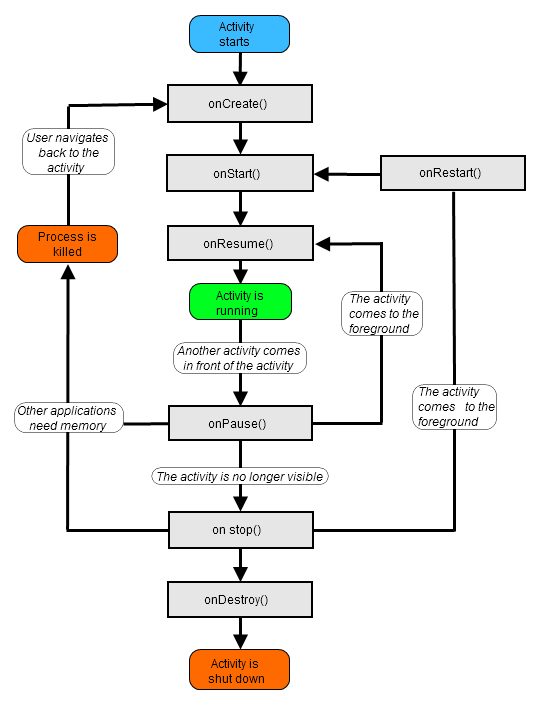
\includegraphics[scale = 0.5]{graphics/lifecycle-activity-android.png}
\caption{Activity Life-Cycle.(\cite{ActivityLifeCycle})}
\label{fig:abb7}
\end{figure}
\subsubsection{Services}
Service ist eine Applikation Komponente, die Operationen im Hintergrund durchf�hrt und keine
Interaktion mit dem Benutzer ben�tigt. Ein Service wird von einer anderen Komponente, wie einer
Activity, gestartet und l�uft auch weiter, wenn die Activity nicht mehr im Vordergrund ist.
\cite[320]{App4U}
\subsubsection{Intents}
Activities und Services werden durch Nachrichten aufgerufen, die eine andere Komponente an sie
sendet. Eine solche Nachricht wird Intent genannt. In einem Intentobjekt werden verschiedene Daten
gespeichert. Jede Intentnachricht hat einen Kontext und ein Ziel. Als Kontext ist die erste
Activity, also die Activity, die die Intentnachricht sendet und als Ziel die Activity, an die die
Nachricht gesendet wurde. Je nach Bedarf k�nnen noch Daten, welche der neuen Activity �bermittelt
werden, in den Intent gespeichert werden, bevor die neue Activity gestartet wird.\cite[321]{App4U}
\subsubsection{Komponenten der Benutzeroberfl�che}
Die Benutzeroberfl�che oder User Interface (UI) in Android Apps besteht aus Views und View Groups.
Views sind Bausteine, wie Textview oder Imageview. View Groups sind Container, die Views oder andere View
Groups enthalten. Um eine bessere Trennung zwischen Design und Java-Code zu erreichen wird das UI in
XML-Dateien definiert. Der verwendete Text der App sollte auch nach M�glichkeit in einer XML-Datei
statt in Java-Code untergebracht werden. Das erleichtert nicht nur das sp�tere �ndern des Textes,
sondern auch die Mehrsprachigkeit einer App. F�r bessere �bersicht empfiehlt es sich, f�r jede
Activity eine XML-Datei mit dem Namen der Activity zu erstellen, welche dann das Layout der Activity
enth�lt.
\subsubsection{Content Provider}
Mechanismus f�r die Persistierung von Daten. Meistens in der Form von SQLite Datenbank auf dem
Endger�t oder in der Cloud.
\subsection{iOS}
Um iOS Apps entwickeln zu k�nnen, braucht man Apples Entwicklungsumgebung Xcode, welche
ausschlie�lich f�r Apple Rechner zur Verf�gung steht. Xcode bringt das aktuelle iOS Software
Development Kit (SDK) mit. In dem iOS SDK sind hochwertige Emulatoren f�r die aktuelle Version
 enthalten und bei Bedarf lassen sich auch �ltere Versionen herunterladen. Apps f�r iOS werden in
 Objective-C und seit kurzem auch mit der von Apple neu eingef�hrten Programmiersprache Swift
 entwickelt. Die \textbf{LLVM} Compiler Infrastruktur ist ein Open Source Projekt und die technische
 Grundlage f�r die native Entwicklung auf iOS (\cite{LLVM}). Xcode wird kostenlos zur Verf�gung
 gestellt.
 Der in Xcode integrierte Interface-Builder unterst�tzt das Drag-and-drop-Verfahren und macht die Gestaltung der Benutzeroberfl�che zu einer relativ
einfachen Aufgabe. In einem Texteditor erfolgt die Eingabe des Quellcodes. Von besonderer Bedeutung
ist die Integration eines iOS-Simulators, auf dem die Anwendung in der gleichen Wiese abl�uft, als
wenn ein tats�chliches iOS-Ger�t die Basis w�re.\\�hnlich wie bei Android wird das
MVC-Entwurfsmuster f�r die Entwicklung von iOS Apps verwendet. F�r Entwicklung mobiler Applikationen ist das
Cocoa-Framework erforderlich, das vielf�ltige h�ufig genutzte Bibliotheken (bspw. zum Zugriff auf
Hardwareger�te) bereitgestellt. Apple stellt mit Cocoa-Touch-Framework eine modifizierte und auf die
Anforderungen leistungsschw�cherer mobiler Endger�te abgestimmte Version des Frameworks zur
Verf�gung. �hnlich wie bei Android werden Apps in einer beschr�nkenden Sandbox ausgef�hrt und es
ist keine direkte Interprozesskommunikation m�glich. Jede App kann nur in einem eigenen Ordner auf
das Dateisystem zugreifen. Anwendungen haben im Standard nur geringe Rechte und der Benutzer muss
die Rechte aktiv best�tigen. Im Folgenden werden die wichtigsten Komponenten der iOS App Entwicklung
vorgestellt.
\\Um f�r die View-Komponenten ein Verhalten zu definieren, stehen drei Mechanismen zur Verf�gung:
\begin{itemize}
  \item Delegation. Erm�glicht eine entkoppelte Kommunikation. 
  \item Target Action. �ber den Target-Action-Mechanismus benachrichtigt die View den Controller,
  wenn bspw. ein Button geklickt wurde.
  \item Notification. Die Kommunikation vom Model an den Controller erfolgt �ber Notifications und
  Key-Value-Observing.
\end{itemize}
\subsubsection{iOS App Lifecycle}
Beim Starten einer iOS App passiert Folgendes:
\begin{enumerate} 
  \item Zuerst wird die main()-Methode in der Klasse main.m ausgef�hrt.
  \item Dann wird die didFinishLaunchingWithOptions()-Methode der Klasse AppDelegate.m ausgef�hrt.
  \item Die Storyboards werden geladen.
  \item Am Ende werden die Methoden viewDidLoad() und viewWillAppear() des ViewControllers, der als
  Start-ViewController festgelegt wurde ausgef�hrt.
\end{enumerate}
\subsubsection{Storyboard}
In dieser Datei lassen sich gleich mehrere Ansichten erstellen und deren �berg�nge (Storyboard
Segues) definieren. Das Storyboard repr�sentiert die View des MVC-Architekturmusters. Die
iOS Benutzerschnittstelle (UI) wird mit einem Interface Builder (UI Builder) gestaltet. Mithilfe
dieses Werkzeugs lassen sich einzelne Komponenten der UI per Drag \& Drop zusammenstellen und mit
einem ViewController verbinden.
Im Ui Builder werden Oberfl�chen nicht nur gezeichnet, sondern auch deren Eigenschaften
definiert. Durch Constraints lassen sich die Positionen der Objekte relativ zueinander beschreiben
und dadurch kann man flexibel mit verschiedenen Aufl�sungen und Darstellungsmodi
(Landscape/Portrait) umgehen.
\begin{figure}[!h]
\centering
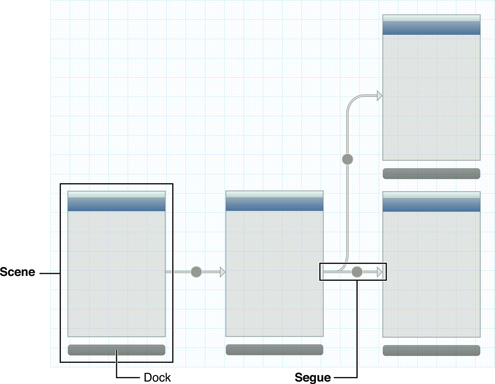
\includegraphics[scale = 0.5]{graphics/storyboard.png}
\caption{Storyboard. Quelle:\cite{DevApple}}
\label{fig:abb12}
\end{figure}
\subsubsection{ViewController}
Die ViewController sind wichtige Bausteine f�r alle iOS-Apps.
Xcode legt bei View-basierten Projekten immer automatisch einen ViewController an, der die
Funktionalit�t des oder eines Controllers innerhalb der App abbildet. 
Die Verwaltung einer Ansicht erfolgt �ber einen ViewController. Ein ViewController beinhaltet die
Gesch�ftslogik einer Anewendung und steuert den Programmablauf (siehe Abb.\ref{fig:abb10}).
Es empfiehlt sich, f�r jeden Dialog einen eigenen ViewController zu nehmen.
ViewController, die im Storyboard definiert wurden, werden
automatisch instanziiert. In Abb.\ref{fig:abb11}
sieht man die Einzelschritte beim Laden einer View.
\begin{figure}[!h]
\centering
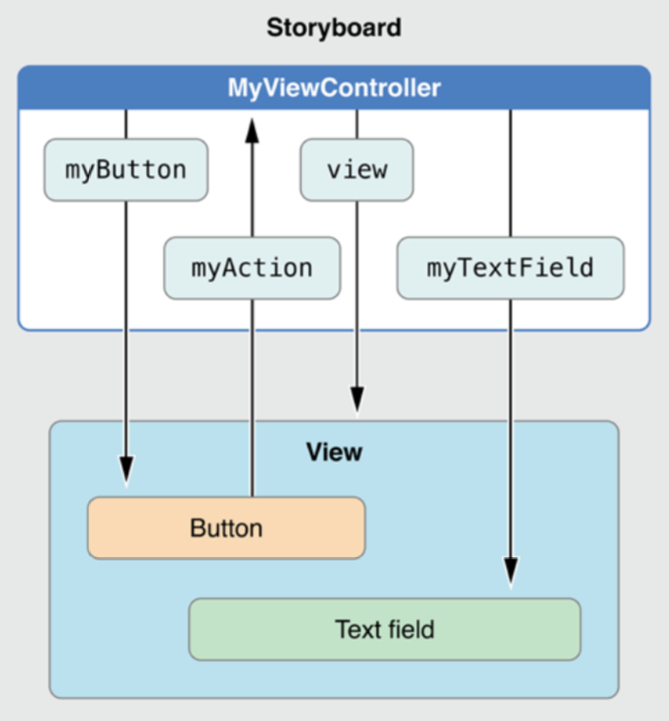
\includegraphics[scale = 0.3]{graphics/ViewController.png}
\caption{Funktionsweise eines ViewControllers. Quelle:\cite{DevApple}}
\label{fig:abb10}
\end{figure}
\begin{figure}[!h]
\centering
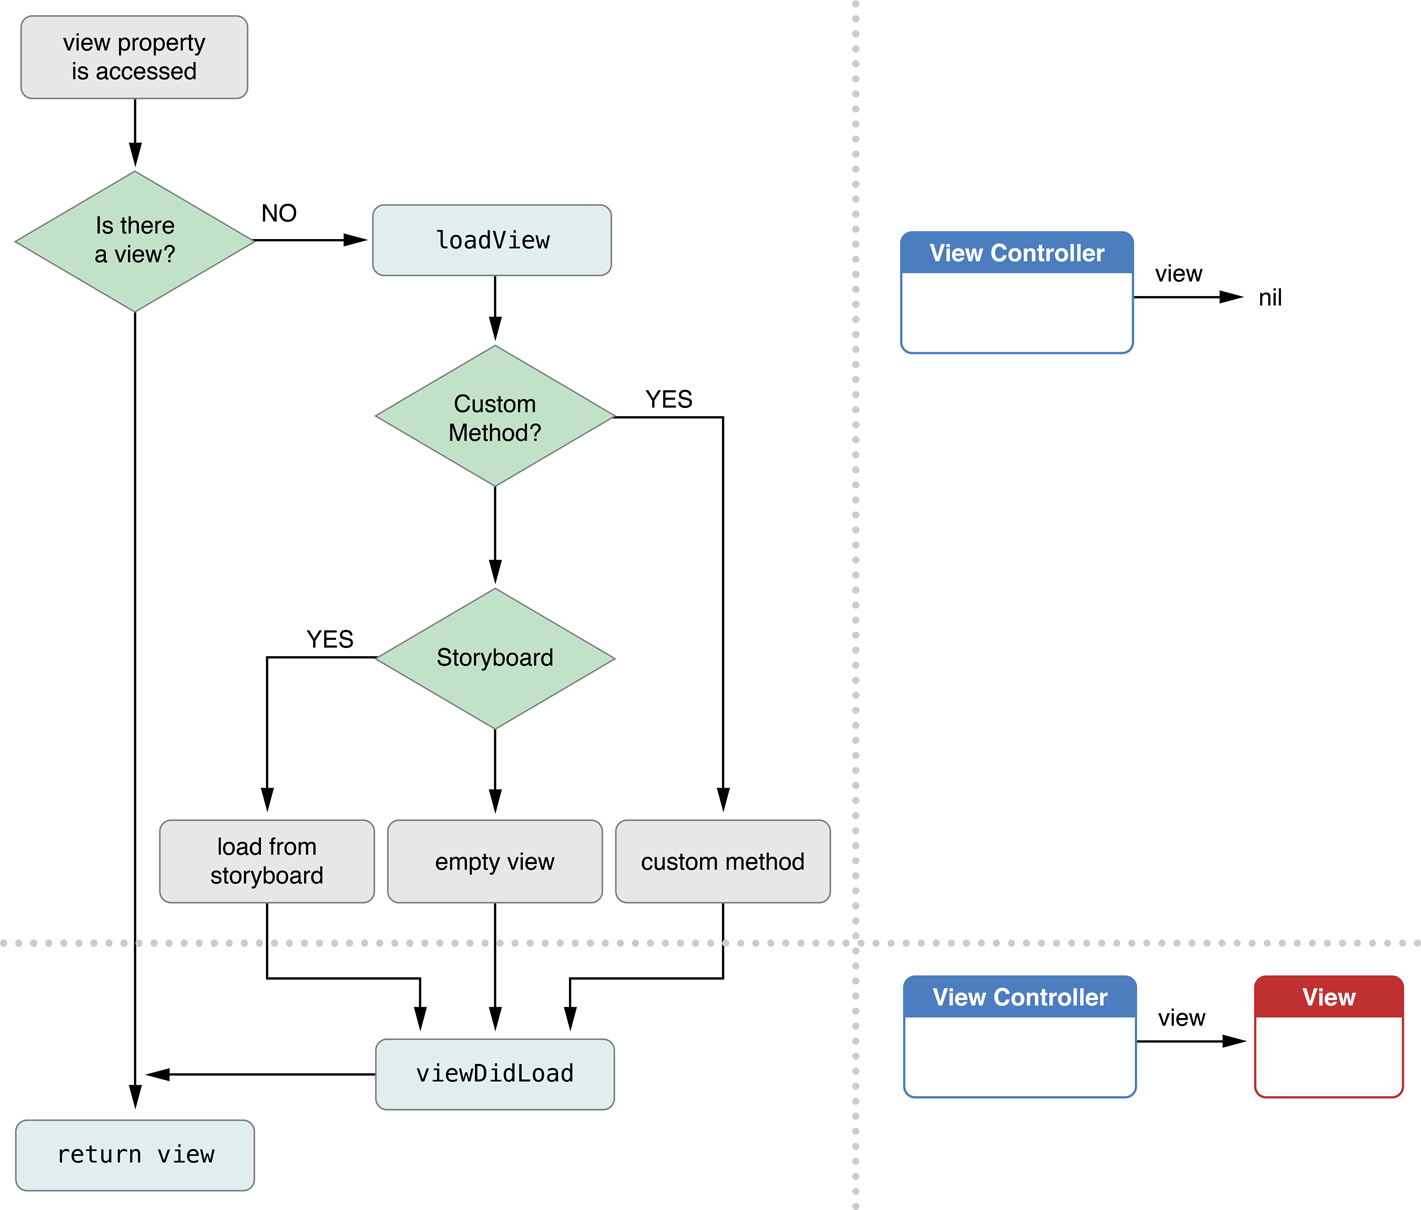
\includegraphics[scale = 0.2]{graphics/loading_a_view_into_memory_2x.png}
\caption{Laden einer View. Quelle:\cite{DevApple}}
\label{fig:abb11}
\end{figure}
\subsubsection{Navigation Controller}
Ein Navigation Controller kapselt die Navigation zwischen ViewControllern. Die ViewController werden
auf einem sogenannten Navigation Stack gestapelt.
\subsubsection{Property Lists ("`Plists"')}
Property Lists sind ein in iOS Apps h�ufig verwendetes Werkzeug um Einstellungen und Zust�nde zu
speichern oder auch mit einer App auszuliefern. Plists stellen eine Hierarchie von strukturierten
Daten dar und werden als XML serialisiert. Xcode bietet einen Editor, mit dem man mittels einer
Benutzeroberfl�che Property Lists bearbeiten kann, ohne sich mit XML Code auseinandersetzen zu
m�ssen. Die Einstellungen eines Projektes werden in einem speziellen File, das \textbf{Info.plist}
gespeichert. Es wird von Xcode generiert und wird beim Start einer App automatisch eingelesen und
ausgewertet.
\subsection{Windows Phone}
Microsoft ver�ffentlichte im Juli 2000 im Rahmen einer umfangreicher Werbekampagne die
sogenannte .NET Plattform. Die .NET Plattform besteht aus den folgenden Komponenten:
\begin{itemize}
  \item Eine Sammlung von Programmiersprachen, wie C\#, Visual C++ .NET, Visual Basic .NET, Visual
  J\# .NET und JScript .NET, sowie die graphische Entwicklungsumgebung Visual Studio.NET. 
  \item Das .NET Framework stellt eine Bibliothek dar, die vorgefertigte Klassen f�r die Entwicklung
  von Web Services, Internet- und Windows-Anwendungen beinhaltet.
  \item .NET Compact Framework ist eine im Funktionsumfang, sowie in den Hardwareanforderungen
  reduzierte Version des .NET Frameworks und ist speziell f�r Ger�te bestimmt, die mit dem mobilen
  Betriebssystem Windows Phone (fr�her Windows CE .NET oder Windows Mobile) arbeiten.
\end{itemize} 
Um Apps f�r Windows Phone entwickeln und auf Ger�ten deployen zu k�nnen, wird eine MSDN Subscription
f�r Entwickler ben�tigt. In dieser Subscription sind die Zugangsrechte f�r Windows Phone Store und
Windows Store bereits f�r die erste Jahreslaufzeit des Abonnements enthalten. Sch�ler und
Studierende, die am Microsoft DreamSpark-Programm teilnehmen, sowie Unternehmen, die f�r das
Microsoft BizSpark-Programm qualifiziert sind, erhalten den Entwickler Account kostenlos. Mit
diesem, sonst kostenpflichtigen Entwicklerkonto hat man nicht nur die M�glichkeit, Apps in den
Windows Phone Store einzureichen und zu �berwachen, sondern auch die Apps auf einem pers�nlichen
Ger�t zu debuggen. Man darf bis zu 10 Apps gleichzeitig installieren, die noch nicht in den Windows
Phone Store eingestellt sind.\\Die .NET Plattform ist, �hnlich wie Java, plattformunabh�ngig.
Mit einer Common Language Specification (CLS) wird genau definiert, wie sich fremde Compiler f�r verschiedene Programmiersprachen bei der
Erzeugung eines speziellen Zwischencodes (MSIL, vergleichbar mit Bytecode von Java) zu verhalten
haben. Der erzeugte MSIL-Code kann auf jedem System ausgef�hrt werden, auf dem eine
.NET-Laufzeitumgebung (CLR-System) installiert ist. Au�er Micorsofts .NET Framework, die
nur f�r Windows angeboten wird, existiert noch das Open Source Projekt "`Mono"', das bspw. auf den
Betriebssystemen Mac OS und Linux lauff�hig ist.
\\�hnlich wie bei iOS von Apple lassen sich Windows Phone Apps ausschlie�lich unter der Verwendung
der Entwicklungsumgebung Visual Studio von Microsoft erstellen. F�r die Installation von Visual Studio wird das Betriebssystem Windows von Microsoft vorausgesetzt. Wie Xcode und Eclipse stellt Visual
Studio eine integrierte Entwicklungsumgebung zur Verf�gung. Im Gegensatz zu den
Entwicklungsumgebungen von iOS und Android ist Visual Studio bis auf die funktional beschr�nkten
Express-Versionen kostenpflichtig. Es wird das kostenlose Windows Phone SDK vorausgesetzt. Nach der
Installation des SDKs, integrieren sich die Tools f�r die Windows Phone-Entwicklung nahtlos in die
bestehende Entwicklungsumgebung Visual Studio. 
Visual Studio bietet Entwurfansicht zur Darstellung der Benutzeroberfl�che und Texteditor f�r die
Eingabe des Quellcodes an.

F�r die Erstellung einer nativen Windows Phone App kann man C\#, Visual
Basic und XAML oder C++ und DirectX verwenden. Man kann auch in Internet Explorer ablaufende Windows Phone-Apps mit HTML5, JavaScript und CSS entwickeln.
Mithilfe des MVVM-Architekturmusters wird eine Separation der
verschiedenen Komponenten erreicht.
\\Die wichtigsten Komponenten einer Windows Phone App sind:
\begin{itemize} 
  \item AssemblyInfo (.vb oder .cs)\\Die Datei enth�lt Metadaten wie die Namen und die Version, die
  anschlie�end in die fertige App generiert werden. Diese Datei gibt es nur f�r C\# oder Visual
  Basic .NET Projekte.
  \item Package.appxmanifest\\Hier werden ebenfalls Informationen wie Name, Beschreibung, Logos und
  ben�tigte Systemfunktionen beschrieben (Metadaten). Die Windows Runtime kann somit die wichtigsten
  Informationen zur Windows-Store-App entnehmen.
  \item Assets\\Dieses Verzeichnis enth�lt ein Standard Logo, Splashscreen und ein Convericon. Diese
  k�nnen durch eigene Dateien mit dem gleichen Namen ersetzt werden.
\end{itemize}
F�r die Gestaltung der Benutzeroberfl�che bietet Visual Studio einen Designer an. Es wird ein
Werkzeugkasten zur Verf�gung gestellt und man kann per Drag \& Drop verschiedene Elemente auf der
App Oberfl�che platzieren. Der Entwickler kann im Designer nur die Oberfl�chenlogik, aber keine
Verarbeitungslogik der eigentlichen Aufgabe. Es entsteht einen XAML-Code \footnotemark[1]. Diese
Trennung verschafft nicht nur eine saubere Aufteilung, sondern auch eine bessere Wartbarkeit und
Wiederverwendbarkeit der einzelnen Komponenten. Zu jeder XAML-Datei (Datei.xaml) gibt es es eine
C\#-Datei, die genau so hei�t (Datei.xaml.cs).
Beim Deklarieren eines Oberfl�cheelements im XAML l�sst sich eine neue Methode in der Code-Behind-
Datei erzeugen. In dieser Methode ist dann die Verarbeitungslogik enthalten.
\footnotetext[1]{XAML (Extensible Application Markup Language) ist eine Dialektform von XML.}  
\cite{MSDNApps}
\cite[125]{App4U}
\cite[382]{MoApp1}
\subsection{Fazit}



\chapter{Cross-Plattform-Entwicklung von mobilen Anwendungen und Stand der Technik}
\section{Was ist Cross-Plattform-Entwicklung - Begriffskl�rung}
\section{Vorstellung und Bewertung der aktuellen Cross-Plattformen}

\cite{10BestCPMDT}
\subsection{PhoneGap}
PhoneGap ist wahrscheinlich der bekannteste Cross-Plattform-Brand. Das Tool ist mittlerweile
Eigentum von Adobe und basiert auf der open source Apache Cordova Projekt. Besonders vorteilhaft
ist, dass es komplett kostenlos ist. Adobe hat eine Enterprise Version von PhoneGap annonciert, bei
der Features via Adobe's Marketing Cloud eingebunden sein werden.
\subsection{Web Apps}
Webbasierte Applikationen werden �ber das Internet angeboten und umgehen so die Restriktionen und
Rahmenbedingungen plattformspezifischer Marktpl�tze. Webanwendungen k�nnen auf jedem beliebigen
mobilen Endger�t ausgef�hrt werden, solange das Endger�t �ber ein Internetbrowser verf�gt. Web Apps
werden auf der Grundlage von HTML, CSS oder JavaScript entwickelt. Die ben�tigen keine Installation
und werden �ber das Internet zur Verf�gung gestellt. Aufgrund fehlender Schnittstellen weisen
Webbasierte Anwendungen einen eingeschr�nkten Zugriff auf die Hardwareressourcen des jeweiligen
Endger�tes auf. Sogenannte hybride Anwendungen basieren zum einen auf einem nativen Kern, der die
Verbindung zu den Hardwareressourcen erm�glicht, und zum anderen auf webbasierten,
plattform�bergreifenden Funktionen. Obwohl spezielle Frameworks die Umwandlung von
plattformunabh�ngigen Anwendungen in native Apps erm�glichen, nutzen viele Hersteller, wie Apple
oder Google, ihre Marktdominanz aus, um hybride Technologien und Frameworks zu verhindern. Weitere
Nachteile von hybride Apps sind die mangelnde Sicherheit und die fehlende Offenheit
\cite[106]{App4U}.
\subsection{Xamarin}
\section{Plattformauswahl}
\chapter{Cross-Plattform-Entwicklung mit Xamarin}
Was ist \textbf{Xamarin}? Xamarin ist ein US-amerikanisches
Softwareunternehmen mit Sitz in San Francisco.
Xamarin bietet eine Entwicklungsumgebung Xamarin Studio und l�sst sich auch alternativ in
Visual Studio als Plugin einbinden. Mit Xamarin.iOS und Xamarin.Android lassen sich native iOS und
Android Apps in C\# programmieren. Damit wird die Entwicklung von Applikationen f�r alle drei
Plattformen in einer einzigen Sprache erm�glicht. Grundlage hierf�r ist das Open-Source-Projekt
\textbf{Mono}. Hierbei wird f�r jede Plattform spezifisch die UI in C\# implementiert. Daraus
entstehen native Oberfl�chen. Bei Android passiert das zur Laufzeit und bei iOS w�hrend des
Kompiliervorgangs. Isoliert betrachtet ist dies bereits ein gravierender Vorteil gegen�ber einer 
plattformspezifischen Entwicklung.
 So wird anstelle von Java, Objective-C und C\# Know-how lediglich Letzteres ben�tigt.
  Dar�ber hinaus vertreibt Xamarin Entwicklungswerkzeuge, mit denen sich auf Basis desselben C\#-
  Codes Apps f�r iOS, Mac OS X, Windows-Systeme und Android erstellen lassen sollen. Au�erdem ist
  das Unternehmen ma�geblich in die Entwicklung der bereits erw�hnten freien .NET-Implementierung
  Mono involviert.
  Xamarin ist 2011 infolge der Entlassung des fr�heren Teams zur Entwicklung von Mono durch Novell entstanden.
Xamarin ist ein unabh�ngiges Unternehmen, aber arbeitet eng mit Microsofts .NET-Team zusammen. Es
gibt eine Partnerschaft zwischen Microsoft und Xamarin, die dazu f�hrt, dass Visual-Studio-Entwickler 
durch Xamarins Produkte zur Entwicklung von Apps f�r iOS und Android unterst�tzt werden. Im Z�ge der 
 Partnerschaft k�nnen MSDN-Abonnenten au�erdem kostenlos auf den Kurs Xamarin University zugreifen, 
 der dabei helfen soll, innerhalb kurzer Zeit zum Experten der Xamarin-Tools zu werden \cite{MX}.
 Das Entwickeln in einer einheitlichen Programmiersprache ist nicht der einzige Vorteil von Xamarin.
 Xamarin.Forms ist ein m�chtiges Feature, mit dem man nicht nur die Anwendung in C\# entwickeln
 kann, sondern man auch den gr��ten Teil des Codes gemeinsam f�r alle drei Zielplattformen nutzen
 kann. Man kann mit Xamarin.Forms in einem Projekt gleichzeitig f�r iOS, Android und Windows Phone
 entwickeln und alle drei Produkte haben am Ende bis zu 70\% gemeinsamen Code und nur 30\%
 plattformspezifischen Code.

\section{Getting Started mit von Xamarin}
Um Xamarin benutzen zu k�nnen, braucht man einen kostenpflichtigen Account. Es gibt verschiedene
Arten von Accounts, die mit unterschiedlichen Features verbunden sind.

In diesem Kapitel werden die drei wichtigsten Bibliotheken von Xamarin vorgestellt. 
Mit Xamarin.iOS / Xamarin.Android erstellte Programme stehen nativen Anwendungen in nichts nach und
k�nnen problemlos in App Store eingestellt werden. F�r erfahrene Entwickler ist der Einstieg in
Xamarin.iOS und Xamarin.Android ganz leicht, da es sich sehr der nativen App-Programmierung �hnelt,
aber im Gegensatz zu der �blichen Programmiersprachen (Objective-C und Java) wird bei Xamarin.iOS
und Xamarin.Android ausschlie�lich C\# benutzt.
Die plattform�bergreifende App-Entwicklung mit Xamarin geht noch weiter. Mit Xamarin.Forms lassen 
sich Apps f�r iOS, Android und Windows Phone mit gemeinsamen Code erstellen. Xamarin.Forms ist jedoch 
nicht f�r alle Typen von Anwendungen geeignet.
\section{Xamarin.iOS}
Mit Xamarin.iOS bietet Xamarin die M�glichkeit, native Apps f�r iOS zu entwickeln. Der Ahead-Of-Time
(AOT) Compiler kompiliert Xamarin.iOS Apps direkt zu nativen ARM Assemblercode, mit anderen Worten,
kann man mit Xamarin native iOS Apps erstellen. Mit Xamarin.iOS hat man quasi die iOS SDK von Apple
in C\# mit .NET Namenskonventionen. Xamarin bietet somit Zugriff auf alle iOS APIs. Dank eines 
automatischen Binding-Generators kann man existierenden Objective-C Code, Frameworks und
benutzerdefinierte Controls problemlos in einer Xamarin App benutzt werden.

\section{Xamarin.Android}
�hnlich wie bei Xamarin.iOS bietet Xamarin.Android die M�glichkeit native Android Apps mit Xamarin
zu erstellen. Xamarin.Android benutzt den sogenannten Just-In-Time (JIT) Compiler um eine
raffinierte Optimierung der App Performance zur Laufzeit zu erm�glichen. Eine Xamarin.Android App
ist eine native Android APK (siehe Abb. \ref{fig:abb19}). Xamarin bringt 100\% von Google�s Android API in C\#
mit.
Mit dem bereits erw�hnten automatischen Binding-Generator kann man Java Code, Frameworks und benutzerdefinierte
Control-Elemente in einer Xamarin App benutzen.
\begin{figure}[!h]
\centering
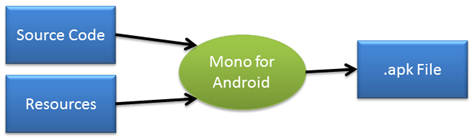
\includegraphics[scale = 0.8]{graphics/Xamarin_Android.png}
\caption{Xamarin.Android (Quelle:\cite{XamAndroid})}
\label{fig:abb19}
\end{figure} 
\\Im Gegensatz zu Xamarin.iOS kann man
Xamarin.Android sowie auf Windows- als auch auf einem Mac-Rechner installieren. Au�er das
aktuelle Android SDK werden bei der Installation von Xamarin.Android auch alle anderen ben�tigten
Komponenten mitinstalliert. Xamarin Studio, bzw. Visual Studio stellt einen Android Emulator zur
Verf�gung, mit dem man eine App debuggen kann.

Genau wie Xamarin.iOS Entwicklung der herk�mmlichen iOS Entwicklung sehr �hnlich ist, ist auch
Xamarin.Android fast identisch mit der nativen Android App Entwicklung. Anstatt Java wird C\#
benutzt, aber die Entwicklungsans�tze sind gleich. Es werden Intents und Activities benutzt und der
Lebenszyklus einer Activity entspricht dem einer Activity aus der nativen Android App Entwicklung.
Die Ressourcen werden auch analog geordnet.
\\Gleich am Anfang, wenn man ein neues Projekt erstellt, sollte man folgende drei Sachen einstellen:
\begin{itemize}
  \item Target Framework - dieses API Level wird zur Kompilierzeit benutzt und legt das Framework
  fest, mit der die App erstellt werden soll.
  \item Minimum Android Version - spezifiziert die �lteste Android Version, die die App unterst�tzen
  soll. Wird zur Laufzeit benutzt.
  \item Target Android Version - spezifiziert die Android Version auf der die App laufen soll. Wird
  zur Laufzeit benutzt.
\end{itemize}
Die verwendeten SDKs m�ssen durch den Open Android SDK Manager von Xamarin Studio (bzw. Visual
Studio) installiert werden.\\Wie bei Xamarin.iOS, bietet Xamarin.Android einen Designer f�r das
Gestalten der Benutzeroberfl�che.
\\\cite{XamAndroid}
\section{Xamarin.Forms: 3 Native UIs, 1 Shared Code Basis}
Bei Xamarin.Forms handelt es sich um ein .NET-basiertes UI Toolkit, mit dem Oberfl�chen entweder in
C\# oder einem speziellen XAML-Dialekt generisch definiert werden. W�hrend des Kompiliervorgangs
entstehen aus dem gemeinsamen Code plattformspezifische, native Benutzeroberfl�chen. Xamarin.Forms
unterst�tzt die Plattformen iOS, Android und Windows Phone, aber (noch) nicht Windows Store Apps. Mit Xamarin.Forms
k�nnen Entwickler deutlich weniger Code schreiben und dadurch wird der jeweilige Mehraufwand pro zu
unterst�tzende Plattform geringer. Allerdings gibt es (noch) keinen UI Designer bei Xamarin.Forms
und man muss die Benutzeroberfl�chen aus dem Code gestalten.
%%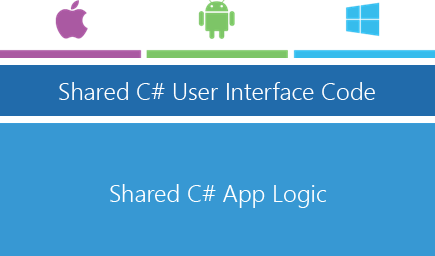
\includegraphics[scale = 0.5]{graphics/XamarinForms1.png}
\\Es gibt zwei
unterschiedliche L�sungsans�tze f�r die plattform�bergreifenden Projekte:
\begin{itemize}
      \item Shared Projects
      \item Portable Class Libraries (PCL)
   \end{itemize}
Bei dem Shared Projects Ansatz wird der enthaltene Code f�r die jeweilige Plattform kopiert und
erneut �bersetzt. Auf diese Weise wird der Code direkt in die Assembly des referenzierenden Projekts
integriert und es wird keine neue Assembly erzeugt. So l�sst sich der Code dieser Assembly auf
mehreren Plattformen wiederverwenden und zugleich �ber Pr�prozessordirektiven oder partielle
Methoden und Klassen in den nativen Projekten auf plattformspezifische Anforderungen eingehen, ohne
zus�tzliche Abstraktionsschichten f�r die nativen Funktionen einbauen zu m�ssen. Allerdings muss
hier erw�hnt werden, dass bei diesem L�sungsansatz die �bersicht im Code schnell verloren geht und
dadurch die Wartbarkeit des Codes erschwert wird. 
\\Bei dem zweiten L�sungsansatz (PCL) bietet sich hingegen die M�glichkeit, mit gemeinsamer
Funktionalit�t ausgew�hlter Zielplattformen gemeinsamen Code in einer Assembly abzubilden. Dadurch
wird ein m�glich effizientes Code Sharing erreicht.
\begin{figure}[!h]
\centering
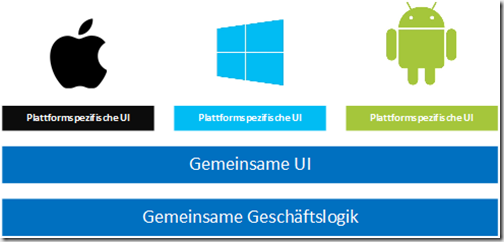
\includegraphics[scale = 0.5]{graphics/xamarin_forms-solution2.png}
\caption{Xamarin.Forms}
\label{fig:abb3}
\end{figure}
\\Die gemeinsame Gesch�ftslogik ist in der
Portable Class Library beinhaltet.
Zus�tzlich werden noch drei weitere Projekte erstellt, eins f�r Android, eins f�r iOS und eins f�r Windows Phone. In den
plattformspezifischen Projekte befinden sich plattformspezifische Views und Logik. Die meisten
Dateien in den plattformspezifischen Projekten werden automatisch generiert. In ganz seltenen F�llen
muss der Entwickler etwas in den plattformspezifischen Projekte hinzuf�gen. Meistens geht es um
Datenbankanbindung oder die Implementierung von Custom Control Renderer, um die von
Xamarin.Forms vorgegebenen Visualisierung von UI Controls zu modifizieren.
%%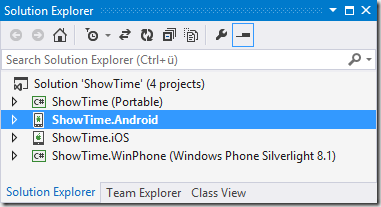
\includegraphics[scale = 0.5]{graphics/xamarin_forms-solution.png}
\\Im Allgemeinen besteht eine Xamarin.Forms Solution aus jeweils einem Projekt pro zu
unterst�tzende Plattform und einem (oder mehreren) plattform�bergreifenden Projekten. 
\begin{figure}[!h]
\centering
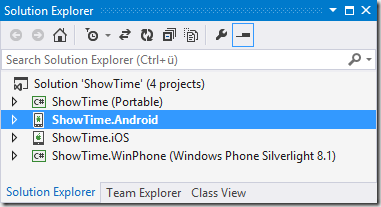
\includegraphics[scale = 0.73]{graphics/xamarin_forms-solution.png}
\caption{Solution}
\label{fig:abb4}
\end{figure}

\section{NuGet und Xamarin Component Store}
Xamarin bietet die M�glichkeit Komponente zu jeder App direkt aus der IDE hinzuzuf�gen.
Somit kann man diverse Controls, Web Service APIs und vieles mehr benutzen. Es k�nnen auch
popul�re Backends wie Microsoft Azure, Parse, Salesforce, SAP usw. in die APP integriert werden,
sowie auch Security Features wie Authentifizierung und Verschl�sselung.

\section{Fazit}
Xamarin.iOS und Xamarin.Android verschaffen direkten Zugriff auf die plattformspezifischen APIs und
dadurch lassen sich Apps erstellen, die spezielle Interaktionen erfordern. Solche Apps haben
die Funktionalit�t und die Leistung einer nativen Anwendung.\\Hingegen ist der Ansatz von
Xamarin.Forms besonders gut f�r Apps geeignet, die wenig plattformspezifische Funktionalit�t
aufweisen oder solche, bei denen keine spezielleren Benutzeroberfl�chen erfordert werden. Also
Anwendungen, bei denen die Gesch�ftslogik h�her priorisiert wird als optische Effekte der
Benutzeroberfl�che, lassen sich ganz bequem mit Xamarin.Forms erstellen. Unter diese Kategorie
fallen die sogenannten Business(Enterprise)-Anwendungen.

\chapter{Cross-Plattform-Entwicklung mit Xamarin am Beispiel einer Migration und
Erweiterung existierender App} 
Um ein Cross-Plattform-Entwicklungsframework gut bewerten zu k�nnen, ist es notwendig eine App zu
entwickeln, die anspruchsvolle Aufgaben erledigt. Am besten w�re es einen Vergleich zwischen zwei
Versionen einer App ziehen zu k�nnen, einer nativ entwickelten Version und einer Version, die mit Xamarin erstellt wurde. 
% Am besten kann man das durchf�hren, indem man eine bereits
% existierende App auf Xamarin migriert, bzw. mit Xamarin neu entwickelt, so dass im
% "`Best-Case-Szenario"' am Ende die Xamarin-App sich kaum von der nativen App unterscheidet. 
% Es
% werden die Anforderungen und Funktionalit�ten einer bereits f�r iOS existierenden Applikation vorgestellt.
% Diese Anwendung wird als Vorlage f�r eine Xamarin.Forms Applikation dienen. Die wichtigsten
% Entwicklungsschritte dieser App werden im darauf folgenden Abschnitt beschrieben.
%
% \\
% \begin{figure}[!h]
% \centering
% 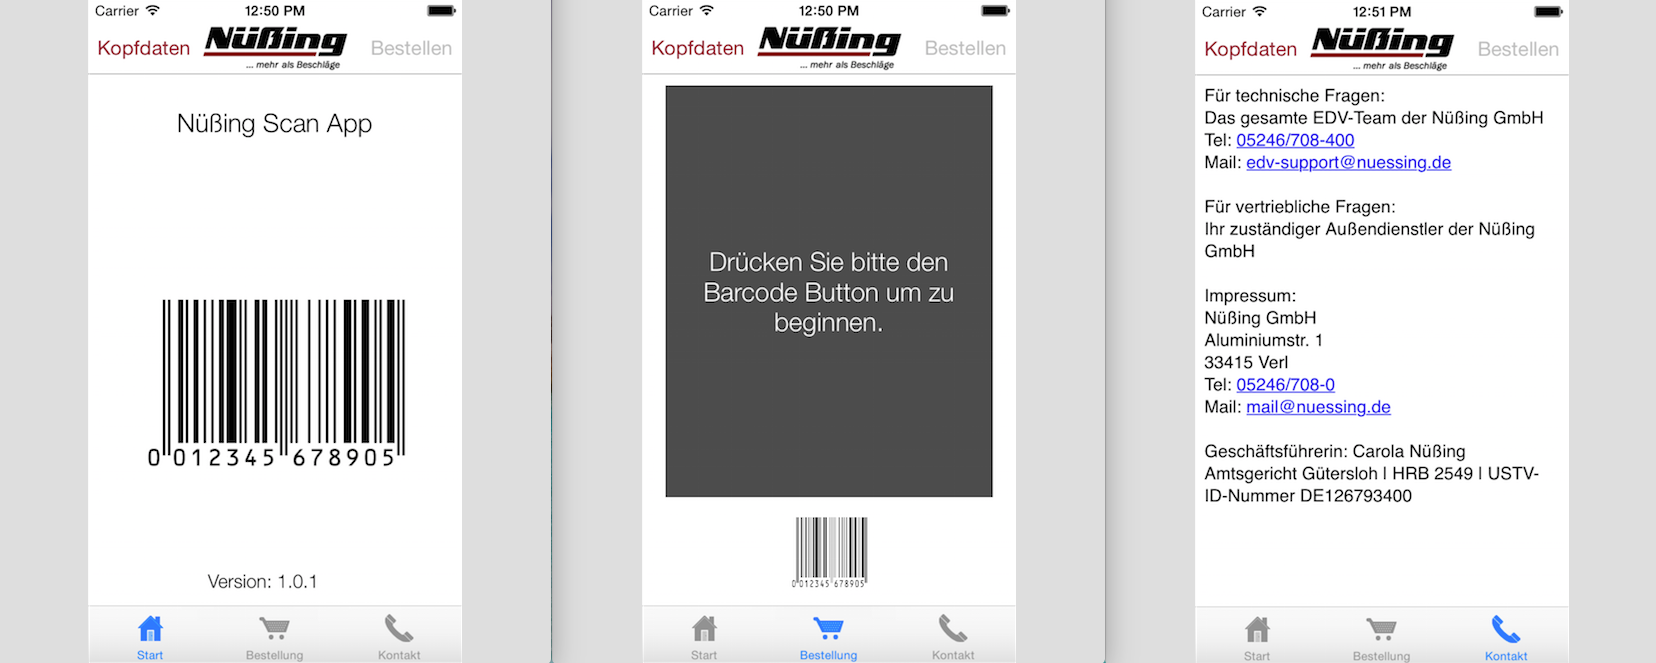
\includegraphics[scale = 0.2]{graphics/ScannAppScreen_1.png}
% \caption{N��ing-Scan-App}
% \label{fig:abb20}
% \end{figure}

\section{Beispiel-Anwendung (Scan-App)}
Gut geeignet f�r den Zweck dieser Arbeit ist eine mobile Anwendung zum Scannen von Barcodes.
Eine solche Anwendung greift auf Hardware-Ressourcen, wie die Kamera des Endger�ts zu.
Ein Benutzer kann mit der App einen Barcode scannen, anschlie�end wird der Barcode beim Server
�berpr�ft und es werden Informationen �ber das Produkt auf dem Bildschirm des Smartphones angezeigt.
Mithilfe der App k�nnen unterschiedliche Artikel ausgew�hlt und bestellt werden.
% N��ing GmbH ist Vollsortimenter f�r Industrie und Handwerk in den Bereichen Beschlagsysteme,
% Bauelemente und Werkzeuge. N��ing bietet seinen Kunden die M�glichkeit an, Artikel mithilfe einer
% App zu bestellen.
% Dank dieser N��ing Scan-App kann ein Handwerker, nach einer einmaligen Registrierung die gew�nschten
% Produkte bestellen. Der Kunde muss lediglich den Barcode des Artikels mit der Kamera des
% Smartphones einscannen. Anschlie�end wird der Barcode beim Server �berpr�ft und falls der Artikel
% erkannt wurde, kann der Kunde die gew�nschte Menge bestellen.
% Bei schlechten Lichtverh�ltnissen l�sst sich die Blitzlicht-Lampe hinzuschalten und im Falle eines
% defekten Barcodes, hat der Kunde auch die M�glichkeit es manuell einzugeben, indem der Kunde die
% Barcodenummer in das daf�r vorgesehene Feld eintr�gt. Nachdem der Kunde eine sechsstellige Zahl
% eingetippt hat, wird automatisch eine Anfrage an den Server gesendet und falls ein Artikel gefunden
% wurde, erscheint eine Beschreibung des Artikels auf dem Bildschirm und der Kunde kann es bestellen
% (siehe Abb.\ref{fig:abb20}).
% \begin{figure}[!h]
% \centering
% 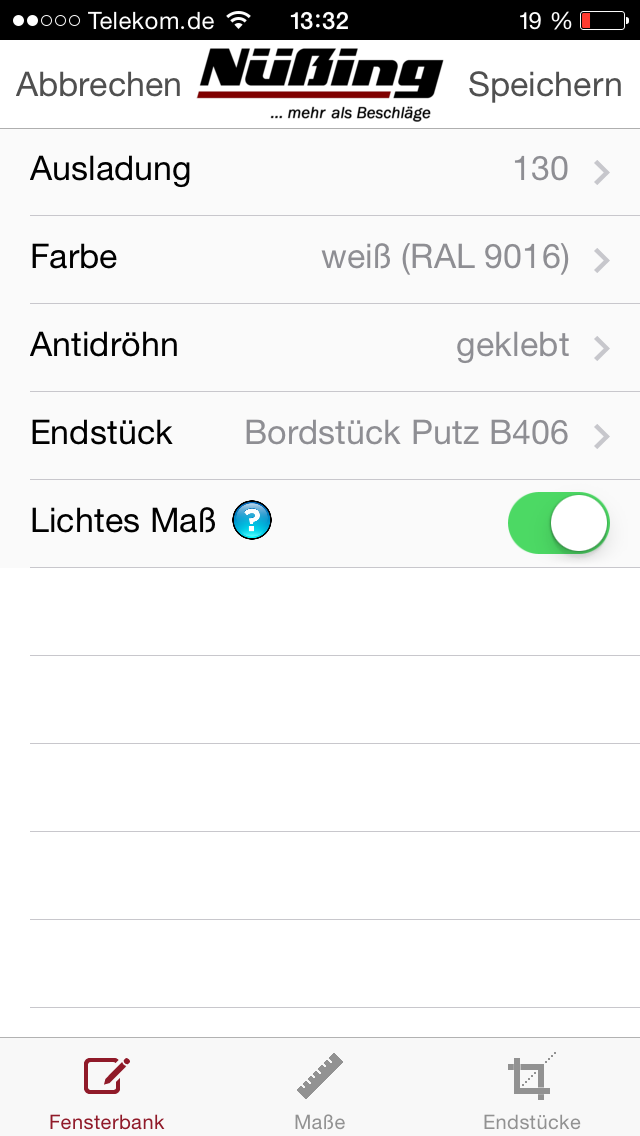
\includegraphics[scale = 0.13]{graphics/NuessingReferenzApp_2.png}
% \caption{N��ing-FensterbankApp Fensterbank Eigenschaften}
% \label{fig:abb21}
% \end{figure}
% \\Die N��ing
% Scan-App (siehe Abb.\ref{fig:abb20}) ist die von der Firma Sunato GmbH entwickelten L�sung dieses
% Problems.
% Es ist eine Applikation (f�r die Apple iOS Plattform), mit der ein Kunde
% (Handwerker) ganz bequem eine Fensterbank bestellen kann, indem er die Ma�e, sowie gew�nschte
% Eigenschaften (Farbe, Antidr�hn, Endst�cke etc.) der Fensterb�nke einfach in sein Smartphone oder
% Tablet eingibt (siehe Abb.\ref{fig:abb21}).
% Beim Absenden einer Bestellung werden die Daten direkt in das N��ing ERP �bertragen und l�sen die
% Bestellung und die Fertigung aus.
F�r die Realisierung des Backends dieser Beispiel-Applikation wird Microsofts
Enterprise Resource Planning (ERP) L�sung, Dynamics AX, eingesetzt.
Die ERP-Software bietet vordefinierte Funktionen f�r die Branchen Fertigung, Gro�handel/Distribution, Einzelhandel und
Dienstleistungen. Der Zugriff auf AX erfolgt mit dem Dynamics AX Workspace als Desktop Client oder
mit dem Enterprise Portal for Microsoft Dynamics AX per Browser. Weiterhin erm�glicht Dynamics AX
den Zugriff �ber eine Reihe von programmierbaren Schnittstellen.\\Die Kommunikation zwischen den
Smartphones und dem AX-System erfolgt mittels Web Services mithilfe einer Schnittstelle, die in AX
definiert wurde.
\\Die App verf�gt �ber eine lokale Datenbank, die f�r das Persistieren der Daten sorgt und den
Bestellprozess unterst�tzt.
% \\Abh�ngig von den Anmeldedaten l�sst sich die Anwendung entweder im normalen Modus (als normaler
% N��ing Kunde) oder im Mitarbeiter Modus. Im Mitarbeiter Packet kann der N��ing Angestellte
% Bestellungen f�r verschiedene Kunden abgeben.
% \cite{Sunato} 

% \begin{figure}[!h]
% \centering
% 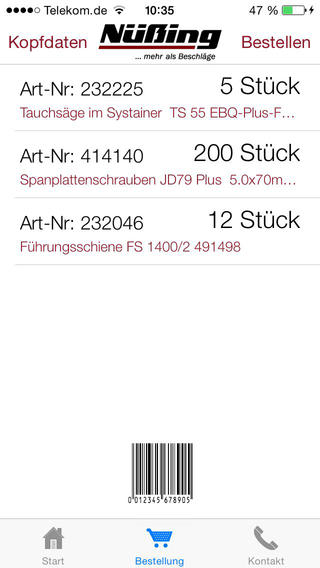
\includegraphics[scale = 0.5]{graphics/ScanAppBestellung.png}
% \caption{N��ing-Scan-App Bestellungspositionen}
% \label{fig:abb22}
% \end{figure}
% \subsection{Technische Grundlagen f�r die Erstellung der Scan-App}
% Es gelten folgende technische Voraussetzungen f�r die ScanApp.
% \begin{itemize}
%   \item \textbf{Backendkommunikation}\\Die App kommuniziert mit den Backend-Services auf AX-Seite
%   �ber HTTP und JSON. Die Serviceadresse wird in der App fest
%   konfiguriert und ist erst durch ein App-Update �nderbar.
% %   \\\cite{WebServicesScanApp}.
%   \item \textbf{Sicherheit}\\Die App unterst�tzt in Produktion eine HTTPS-Kommunikation. Das
%   erm�glicht einen relativ sicheren Betrieb der App in einer unsicheren Umgebung.
%   \item \textbf{Anmeldeprozess}\\Die Registrierung dient der eindeutigen Identifikation und
%   Freischaltung eines App-Benutzers. Als Anmeldedaten werden Kundennummer und PLZ von dem Benutzer
%   beim erstmaligen App-Start eingegeben. Die Daten werden beim Backend �berpr�ft und wenn die
%   Registrierung erfolgreich ist, bekommt die App eine g�ltige GUID. Diese wird als
%   Session-ID f�r die weitere Kommunikation mit dem Backend benutzt und in der App dauerhaft
%   gespeichert. Sollte die Anmeldung nicht erfolgreich sein (z.B. Kundennummer falsch), ist die GUID
%   auf "`String.Empty"' gesetzt. Auf diesem Weg weist die App den Benutzer hin, dass seine
%   Anmeldedaten nicht akzeptiert worden sind und er die Anmeldung wiederholen kann bzw. soll.
%   \item \textbf{Bestellprozess}\\
%   Bei einem Klick auf den "`Bestellen"' Button werden die Auftragsdaten (Kundennummer,
%   Kundenname, Telefon, Lieferterminwunsch, Kommission, Bestellpositionen) an den Bestellservice �bermittelt und der Server best�tigt den erfolgreichen Eingang oder gibt, gegebenfalls, Auskunft �ber einen
%   Fehler. F�r diesen Zweck wurde eine R�ckgabestruktur mit R�ckgabecodes von dem Server
%   definiert.
%    Das Lieferdatum wird automatisch auf das Tagesdatum gesetzt. Sollte der Benutzer sich
%    ein anderes Lieferdatum w�nschen, kann er den Liefertermin auf das von ihm ausgew�hlte Datum
%    setzen.
%    Diese Daten werden von der App gespeichert und bei den weiteren Bestellungen als Stammdaten mit
%    den gespeicherten Werten vorbelegt. Im Gegensatz dazu wird der Wert einer bei der Bestellung
%    angegebenen Kommission nicht gespeichert und muss bei jeder Bestellung neu angegeben werden.
% \end{itemize}
% \subsection{Erweiterung der Scan-App}
% Die ScanApp soll auf Xamarin migriert und um folgende Funktionalit�ten erweitert werden:
% \begin{itemize}
%   \item Die Bestelldaten sollen um ein Feld "`Email"' erweitert werden. Die Emailadresse soll
%   ebenso wie Name und Telefonnummer nach einmaligen Eintippen gespeichert bleiben und bei jeder
%   Bestellung mitgesendet werden. Auf diese Weise kann N��ing eine Eingangsbest�tigung an diese
%   Emailadresse schicken.
%   \item Wenn man im Mitarbeiterpaket eine Kundennummer eingibt, soll der Name des Kunden mit dieser
%   Kundennummer aus dem AX-System geholt und angezeigt werden. Ziel dieser Erweiterung ist es  zu
%   vermeiden, dass der falsche Kunde als K�ufer eingetragen wird, im Falle eines Zahlendrehers.
%   \item Die Men�steuerung soll ge�ndert werden. Anstatt die bisherige vertikale tab-basierte
%   Navigation soll ein barrierefreies horizontales Dropdown Navigationsmen� (�hnlich wie das
%   sogenannte Hamburger-Menu) angewendet werden. Das w�rde eine Erweiterung der Navigationspunkte des Men�s erlauben. Bei dieser
%   Men�variante ist das Men� versteckt und wird erst beim Tippen auf den Men�-Button (oder beim
%   Wischen von links nach rechts) aufgeklappt.
%   \item Au�er Scannen, manuelle Eingabe, Warenkorb und Kontakseite, soll man noch die
%   M�glichkeit haben, zu drei weitere Seiten zu navigieren:
%   \begin{itemize}
%     		\item Favoriten
%     		\item Scan Historie - hier werden die gescannten Barcodes aufgelistet.
%     		\item Abgeschlossene Bestellungen
%   \end{itemize}
%   \item �nderung bei manuellen Eingabe: Es soll m�glich sein eine beliebigstellige Barcodenummer
%   eintippen und �berpr�fen k�nnen (Zur Zeit ist es auf einen sechsstelligen Barcode eingeschr�nkt). 
%   \item �nderung bei der �berpr�fung eines Barocodes: Es gibt unterschiedliche Artikel, die
%   die gleiche Barcodenummer haben. In solchen F�llen sollen die Artikel aufgelistet werden, so dass
%   der Kunde den passenden Artikel ausw�hlen kann.
% \end{itemize}
\section{Anforderungsanalyse}\label{Anforderungsanalyse}
Neben triviale Anforderungen, wie bspw. die App soll nummerische, sowie alpha-nummerische
Eingabefelder anbieten, gibt es einige sehr anspruchsvolle und f�r die Evaluierung des
Cross-Plattform-Entwicklung-Frameworks interessante Anforderungen.
\newline \textbf{Problemstellung:} Die Scan-App ist vorwiegend f�r Handwerker vorgesehen, die oft
Kunden von gro�en Vorsortimenter sind. Sie m�ssen oft Produkte anhand einer Barcodenummer bestellen.
Das Aufschreiben dieser Barcodenummern auf Papier ist m�hsam und fehlertr�chtig. Eine Bestellung
kann dann telefonisch oder online abgeschlossen werden.\\Im ersten Fall muss der Kunde hoffen, dass
die Telefonleitungen nicht besetzt sind und au�erdem kann die akustische �bermittlung der
Barcodenummern zu weiteren Problemen f�hren.\\Eine Bestellung online abzuschlie�en, scheint die
sichere Variante zu sein, allerdings muss der Kunde sich erstmal einen Zugang zu einem PC mit
Internetanschluss erschaffen, sich anschlie�end anmelden, die ben�tigten Formulare ausf�llen und
erst dann kann der Kunde die Bestellung abschlie�en.
\newline \textbf{Motivation:} Entlastung der Kunden.
\newline \textbf{L�sung:} Eine mobile Anwendung, mit der Handwerker sofort und direkt vor Ort
Barcodes mit ihren Smartphones einscannen k�nnen und anschlie�end eine Bestellung quasi per
Knopfdruck absenden k�nnen.
\newline \textbf{Anforderungen an die App:}
\\A 1. Nach der Installation der App, wird der Benutzer
aufgefordert sich zu Registrieren und erst dann wird die Anwendung freigeschaltet.
\\A 2. Bei der Registrierung wird beim Backend eine eindeutige GUID generiert, die in der App
Datenbank gespeichert wird. Diese GUID wird als Session-ID f�r die weitere Kommunikation mit dem
Backend benutzt.
\\A 3. Eine "`frei geschaltete"' Scan-app startet mit der "`Men�"'-Ansicht.
\\A 4. F�r die Men�f�hrung wird ein barrierefreies horizontales Dropdown Navigationsmen� (bekannt
auch als Hamburger-Menu) angewendet werden. Das w�rde eine Erweiterung der Navigationspunkte des
Men�s erlauben. Bei dieser Men�variante ist das Men� versteckt und wird erst beim Tippen auf den
Men�-Button (oder beim Wischen von links nach rechts) aufgeklappt.
\\A 5. Das Men� enth�lt folgende Navigationspunkte:
\begin{itemize}
  \item Bestellungsdaten (Pers�nliche Daten)
  \item Bestellungskopfdaten
  \item Scannen
  \item Manuelle Eingabe
  \item Favoritenlisten
  \item Warenkorb Ansehen
  \item Scan Historie
  \item Abgeschlossene Bestellungen
  \item Kontakt
\end{itemize}
A 6. Der Benutzer muss seine pers�nliche Daten (Name, Email, Telefonnummer) ausf�llen und
speichern, bevor er eine Bestellung abschlie�en kann.
\\A 7. Die App �berpr�ft die Eingaben des Benutzers und weist den User auf ung�ltige Eingaben hin.
Zum Beispiel eine Email Adresse ohne "`@"'-Zeichen.
\\A 8. Die Bestellungskopfdaten sind optional. Da kann der User einen expliziten Liefertermin
angeben, sowie weitere Notizen an das Backend �bermitteln, wie z.B. eine andere Lieferadresse.
\\A 9. Die optionalen Bestellungskopfdaten werden bei einem erfolgreichen Abschluss einer Bestellung
auf die Default-Werte (Kein expliziter Liefertermin, Notiz wird auf String.Empty gesetzt)
zur�ckgesetzt.
\\A 10. Die App bietet eine "`Kontakt"'-Ansicht mit einer Web-View an, in der der User die
M�glichkeit hat mit einem Klick auf den entsprechenen Link den Support anzurufen oder eine Email zu verfassen.
\\A 11. Der User kann einen Barcode mithilfe seiner Smartphonekamera scannen oder es manuell
eingeben.
\\A 12. Die App speichert alle eingescannten oder manuell eingegebenen Barcodenummern, die beim
Server �berpr�ft worden sind und f�hrt eine Scan Historie, in der Datum und Zeit (sekundengenau)
der Barcode�berpr�fung vermerkt werden.
\\A 13. Wenn unter einer Barcodenummer mehrere Artikel gefunden werden, werden die Beschreibungen
der Produkte aufgelistet, so dass der Benutzer den passenden Artikel ausw�hlen kann. 
\\A 14. Der User kann die Scanhistorie
ansehen und bei Klick auf eine Barcodenummer, wird die Nummer erneut beim Backend �berpr�ft, so dass bei Verf�gbarkeit des Produkts es in den Warenkorb
gelegt werden kann.
\\A 15. In der "`Warenkorb"'-Ansicht hat der User die M�glichkeit auf eine Bestellposition zu
klicken und anschlie�end die Menge �ndern, die Bestellposition l�schen oder das Produkt zu seiner Favoriten
hinzuf�gen. 
\\A 16. In der "`Favoriten"'-Ansicht sieht man eine Beschreibung der Favoriten-Artikel und bei Klick
auf einen Artikel, wird das Produkt, identisch wie bei der Scanhistorie, beim Server �berpr�ft und der
App-Nutzer hat dann die M�glichkeit, es zum Warenkorb hinzuzuf�gen. 
\\A 17. Die Applikation kommuniziert mittels Web Services mit dem Server.
\\A 18. Die App generiert mithilfe des Verschl�sselungsalgorithmus SHA-256 einen Adresszusatz f�r
die Web Services URI, um eine Kommunikation mit dem Backend zu erm�glichen.
\\A 19. Die Anwendung kann auf die Kamera, inkl. das Blitzlicht des Ger�tes zugreifen.
\\A 20. Die Daten k�nnen permanent gesichert werden.
\\A 21. Die App, kann in den plattformeigenen App-Stores (Google Play Store und Apples App Store)
ver�ffentlicht werden.
\newline \textbf{Ausgrenzungen:}
\newline L 1.
Die Entwicklung des Backends geh�rt nicht dazu.
\newline \textbf{Annahmen:}
\newline P 1. Jeder Kunde hat einen Smartphone mit Zugang zum mobilen Internet.

\section{Anwendungsf�lle}
Im Folgenden werden Anwendungsf�lle (Use
Cases) der Scan-App aufgef�hrt (siehe Abb. \ref{fig:abb20}). Mithilfe dieser Use Cases werden die
Eigenschaften und funktionale Anforderungen an die Scan-App ermittelt. Ein Scan-App Benutzer ist ein
Mensch, der durch die App Informationen �ber Produkte anhand einer Barcodenummer (eingescannt oder
manuell eingegeben) bekommen kann und anschlie�end das entsprechende Produkt bestellen kann.

\begin{figure}[!h]
\centering
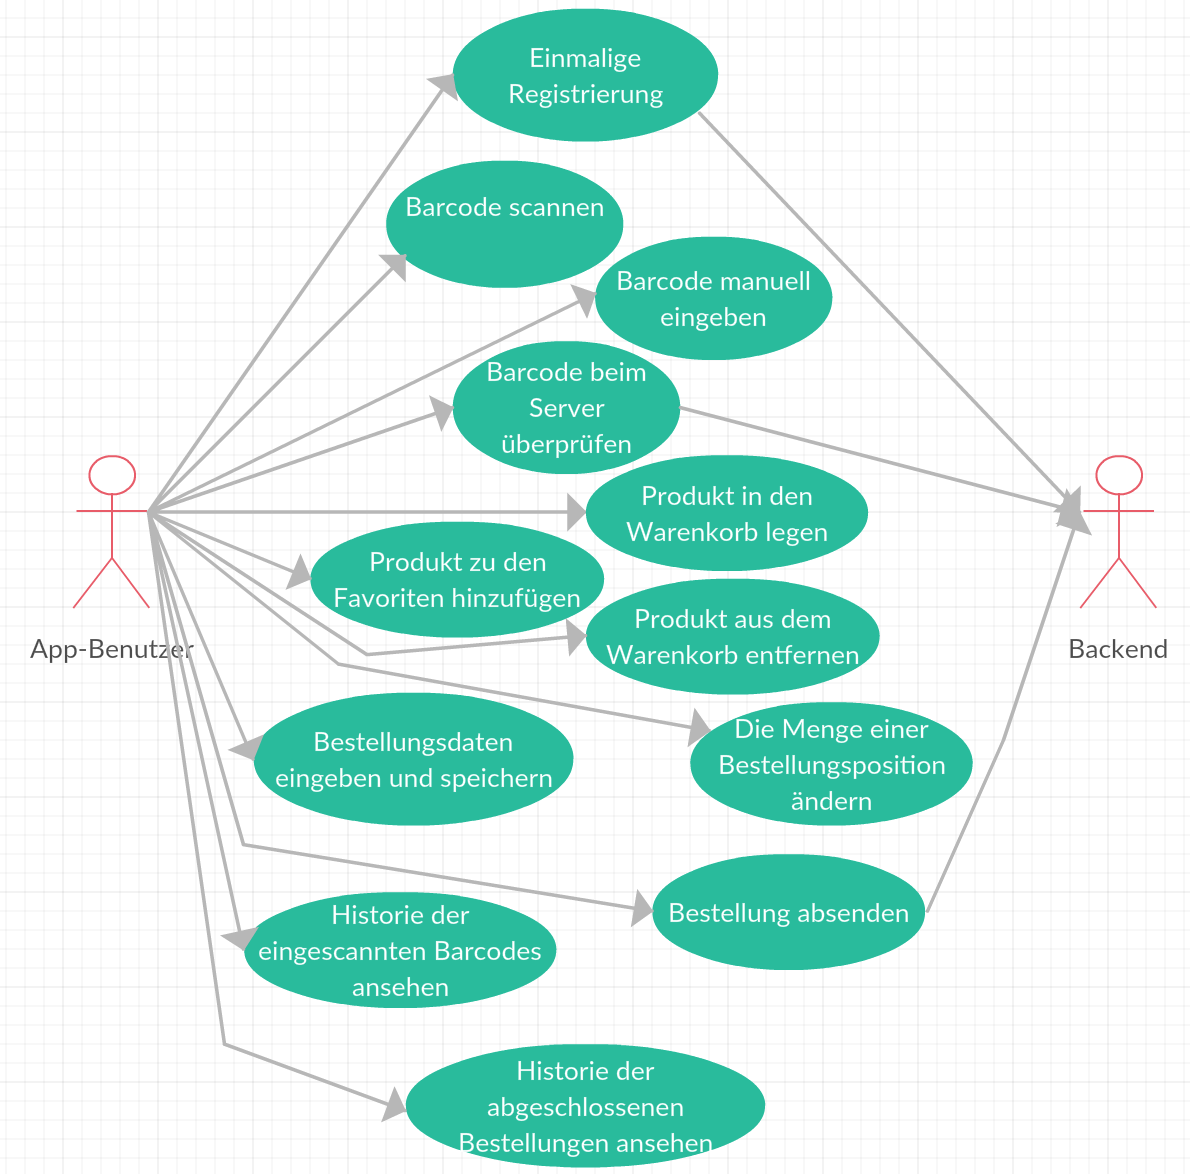
\includegraphics[scale = 0.65]{graphics/UseCases.png}
\caption{Anwendungsf�lle der ScanApp}
\label{fig:abb20}
\end{figure}

\subsection{Use Case: Einmalige Registrierung}
% \textbf{Titel: Einmalige Registrierung}
\textbf{Akteure:} Benutzer der App, der Server auf der Backendseite
\newline \textbf{Ziel:} Der Benutzer meldet sich an und ist somit f�r die Benutzung der App
freigeschaltet.
% \newline \textbf{Ausl�ser:} Der Benutzer m�chte die App freischalten.
\newline \textbf{Vorbedingungen:} Die Scan-App wurde heruntergeladen und installiert.
\newline \textbf{Nachbedingungen:} Der User kann die App benutzen.
\newline
\newline \textbf{Erfolgsszenario:} 
\begin{enumerate}
  \item Der User tippt seine Kundennummer und seine Postleitzahl ein und
  auf dr�ckt den "`Registrieren"'-Button.
  \item Beim Backend werden die Angaben des Benutzers �berpr�ft.
  \item Der Server best�tigt die Registrierung und sendet eine eindeutige GUID.
  \item Das System speichert diese GUID in der Datenbank der Scan-App.
  \item Das System zeigt die "`Menu"'-Ansicht der App an. D.h. die App wird "`frei
  geschaltet"'.
\end{enumerate} 
\textbf{Fehlerf�lle:} 

1.a) Der Server gibt Auskunft �ber einen Fehler. Weiter -> Erfolgsszenario: 1.
\subsection{Use Case: Barcode scannen}
% \textbf{Titel:} Barcode scannen
\textbf{Akteure:} Benutzer der App
\newline \textbf{Ziel:} Der Benutzer hat einen Barcode mithilfe seiner Smartphonekamera eingescannt.
% \newline \textbf{Ausl�ser:} Der Benutzer m�chte die App freischalten.
\newline \textbf{Vorbedingungen:} Die Scan-App wurde installiert und freigeschaltet.
\newline \textbf{Nachbedingungen:} Der Barcode wurde eingescannt und dauerhaft auf dem Ger�t
gespeichert.
\newline
\newline \textbf{Erfolgsszenario:} 
\begin{enumerate}
  \item Der User navigiert zu der "`Scan"'-Ansicht.
  \item Das System zeigt die Ansicht an.
  \item Der Benutzer dr�ckt den "`Starte Scanner"'-Button.
  \item Das System startet die Kamera des Ger�ts.
  \item Der Benutzer richtet den Fokus der Kamera auf den Barcode.
  \item Der Barcode wird erfasst.
  \item Das System zeigt den gescannten Barcode wird an.
  \item Das System speichert den Barcode in der Datenbank der App.
\end{enumerate} 
\textbf{Fehlerf�lle:} 

5.a) Barcode konnte nicht eingescannt werden. Weiter -> Erfolgsszenario: 2.
\subsection{Use Case: Barcode manuell eingeben}
\textbf{Akteure:} Benutzer der App
\newline \textbf{Ziel:} Der Benutzer m�chte einen Barcode manuell eintippen.
\newline \textbf{Vorbedingungen:} Die Scan-App wurde installiert und freigeschaltet.
\newline \textbf{Nachbedingungen:} Der Barcode wurde dauerhaft auf dem Ger�t
gespeichert.
\newline
\newline \textbf{Erfolgsszenario:} 
\begin{enumerate}
  \item Der User navigiert zu der "`Manuelle Eingabe"'-Ansicht.
  \item Das System zeigt die Ansicht an.
  \item Der Benutzer tippt die Barcodenummer in das daf�r vorgesehene Feld ein.
  \item Das System speichert den Barcode in der Datenbank der App.
\end{enumerate} 
\subsection{Use Case: Barcode beim Server �berpr�fen}
\textbf{Akteure:} Benutzer der App, Server
\newline \textbf{Ziel:} Der Benutzer m�chte Information �ber einen Barcode bekommen.
\newline \textbf{Vorbedingungen:} 
\begin{itemize} 
  \item Die Scan-App wurde installiert und freigeschaltet.
  \item Der Benutzer befindet sich in der "`Scan"'- oder
"`Manuelle Eingabe"'-Ansicht der App und Barcodenummer wurde eingescannt bzw. manuell eingegeben.
\end{itemize} 
\textbf{Nachbedingungen:} Es werden Informationen �ber das Produkt, zu dem die
Barcodenummer geh�rt, angezeigt.
\newline
\newline \textbf{Erfolgsszenario:} 
\begin{enumerate}
  \item Der Benutzer dr�ckt den "`Code Abfrage"'-Button.
  \item Die Barcodenummer wird beim Server �berpr�ft.
  \item Der Server gibt Auskunft �ber die Abfrage.
  \item Das System zeigt auf dem Bildschirm des Smartphones Informationen (Beschreibung,
  verf�gbare Menge) �ber das Produkt an.
\end{enumerate} 
\textbf{Fehlerf�lle:} 

2.a) Ein Netzwerk ist aufgetreten. Weiter -> Erfolgsszenario: 1.
\subsection{Use Case: Produkt in den Warenkorb legen}
\textbf{Akteure:} Benutzer der App
\newline \textbf{Ziel:} Der Benutzer m�chte einen Artikel in den Warenkorb legen.
\newline \textbf{Vorbedingungen:}
\begin{itemize} 
  \item Die Scan-App wurde installiert und freigeschaltet.
  \item Der Benutzer befindet sich in der "`Produkt Information"'-Ansicht
der App, eine Barcodenummer wurde eingescannt bzw. manuell eingegeben und beim Server �berpr�ft.
  \item Aus der Information �ber das Produkt ist zu entnehmen, dass das Produkt
verf�gbar ist.
\end{itemize} 
\textbf{Nachbedingungen:} Das Produkt befindet sich im Warenkorb.
\newline
\newline \textbf{Erfolgsszenario:} 
\begin{enumerate}
  \item Der User gibt die gew�nschte Menge in das daf�r vorgesehene Feld ein.
  \item Der Benutzer dr�ckt den "`Warenkorb"'-Toolbarbutton.
  \item Das System best�tigt durch ein Popup Fenster das Einf�gen des Produkts in den Warenkorb.
\end{enumerate} 
\subsection{Use Case: Produkt zu den Favoriten hinzuf�gen}
\textbf{Akteure:} Benutzer der App
\newline \textbf{Ziel:} Der Benutzer m�chte einen Artikel zu seinen Favoriten hinzuf�gen.
\newline \textbf{Vorbedingungen:} 
\begin{itemize} 
  \item Die Scan-App wurde installiert und freigeschaltet.
  \item Der Warenkorb ist nicht leer
\end{itemize} 
\textbf{Nachbedingungen:} Das Produkt befindet sich in der Liste der Favoriten.
\newline
\newline \textbf{Erfolgsszenario:} 
\begin{enumerate}
  \item Der User navigiert zum Menupunkt "`Warenkorb ansehen"'.
  \item Das System zeigt die "`Warenkorb"'-Ansicht an. Die Bestellungspositionen erscheinen in Form
  einer Liste.
  \item Der Benutzer tippt auf den gew�nschten Artikel.
  \item Das System �ffnet eine neue Ansicht, in der der User M�glichkeit hat eine neue Menge
  anzugeben, das Produkt aus der Warenkorbliste zu entfernen oder es zu der Liste seiner Favoriten hinzuzuf�gen.
  \item Der Benutzer dr�ckt den "`Favoriten"'-Toolbarbutton.
  \item Das System f�gt das Produkt zu der Liste der Favoriten hinzu.
\end{enumerate}
\textbf{Fehlerf�lle:} 

6.a) Das System meldet durch ein Popup Fenster, dass das Produkt sich bereits in der Liste der
Favoriten befindet.
\subsection{Use Case: Produkt aus dem Warenkorb entfernen}
\textbf{Akteure:} Benutzer der App
\newline \textbf{Ziel:} Der Benutzer m�chte einen Artikel aus dem Warenkorb entfernen.
\newline \textbf{Vorbedingungen:}
\begin{itemize} 
  \item Die Scan-App wurde installiert und freigeschaltet.
  \item Der Warenkorb ist nicht leer
\end{itemize} 
\textbf{Nachbedingungen:} Das Produkt befindet sich nicht mehr im Warenkorb.
\newline
\newline \textbf{Erfolgsszenario:} 
\begin{enumerate}
  \item Der User navigiert zum Menupunkt "`Warenkorb ansehen"'.
  \item Das System zeigt die "`Warenkorb"'-Ansicht an. Die Bestellungspositionen erscheinen in Form
  einer Liste.
  \item Der Benutzer tippt auf die gew�nschte Bestellungsposition.
  \item Das System �ffnet eine neue Ansicht, in der der User M�glichkeit hat eine neue Menge
  anzugeben, das Produkt aus der Warenkorbliste zu entfernen oder es zu der Liste seiner Favoriten hinzuzuf�gen.
  \item Der Benutzer dr�ckt den "`L�schen"'-Toolbarbutton.
  \item Das System entfernt das Produkt aus dem Warenkorb und �ffnet die "`Warenkorb"'-Ansicht.
\end{enumerate} 
\subsection{Use Case: Die Menge einer Bestellungsposition �ndern}
\textbf{Akteure:} Benutzer der App
\newline \textbf{Ziel:} Der Benutzer m�chte die Menge einer Bestellungsposition �ndern.
\newline \textbf{Vorbedingungen:}
\begin{itemize} 
  \item Die Scan-App wurde installiert und freigeschaltet.
  \item Der Warenkorb ist nicht leer
\end{itemize} 
\textbf{Nachbedingungen:} Die neue Menge der Bestellposition wurde gespeichert.
\newline
\newline \textbf{Erfolgsszenario:} 
\begin{enumerate}
  \item Der User navigiert zum Menupunkt "`Warenkorb ansehen"'.
  \item Das System zeigt die "`Warenkorb"'-Ansicht an. Die Bestellungspositionen erscheinen in Form
  einer Liste.
  \item Der Benutzer tippt auf die gew�nschte Bestellungsposition.
  \item Das System �ffnet eine neue Ansicht, in der der User M�glichkeit hat eine neue Menge
  anzugeben, das Produkt aus der Warenkorbliste zu entfernen oder es zu der Liste seiner Favoriten hinzuzuf�gen.
  \item Der Benutzer tippt eine neue Menge in das daf�r vorgesehene Feld ein.
  \item Der Benutzer dr�ckt den "`Zur�ck"'-Button. D.h. der Benutzer m�chte zur�ck zu der
  "`Warenkorb"'-Ansicht navigieren.
  \item Beim Verlassen der Ansicht speichert das System die neue Menge.
  \item Das System zeigt die aktualisierte "`Warenkorb"'-Ansicht an.
\end{enumerate} 
\subsection{Use Case: Bestellungsdaten eingeben und speichern}
\textbf{Akteure:} Benutzer der App
\newline \textbf{Ziel:} Der Benutzer m�chte seine
Bestellungsdaten ausf�llen, weil die erforderlich f�r das Absenden einer Bestellung sind.
\newline \textbf{Vorbedingungen:} Die Scan-App wurde installiert und freigeschaltet.
\newline \textbf{Nachbedingungen:} Die Bestellungsdaten wurden in der App-Datenbank gespeichert.
\newline
\newline \textbf{Erfolgsszenario:} 
\begin{enumerate}
  \item Der User navigiert zum Menupunkt "`Bestellungsdaten"'.
  \item Das System zeigt die "`Bestellungsdaten"'-Ansicht an.
  \item Der Benutzer f�llt die Eingabefelder (Name, Email, Telefonnummer, Lieferadresse) aus.
  \item Der Benutzer dr�ckt den "`Speichern"'-Toolbarbutton.
  \item Das System speichert die Daten und best�tigt es mit einem Popup Fenster.
\end{enumerate}
\textbf{Fehlerf�lle:} 

5.a) Das System meldet durch ein Popup Fenster, dass die eingegebene Daten nicht den korrekten
Format haben. Weiter -> Erfolgsszenario: 3.
\subsection{Use Case: Bestellung abschlie�en}
% \textbf{Titel: Bestellung abschlie�en}
\textbf{Akteure:} Benutzer der App, der Server auf der Backendseite
\newline \textbf{Ziel:} Der Benutzer m�chte eine Bestellung abschlie�en.
% \newline \textbf{Ausl�ser:} Der Benutzer m�chte eine Bestellung abschlie�en.
\newline \textbf{Vorbedingungen:}
\begin{itemize} 
  \item Die Scan-App wurde
installiert und freigeschaltet.
  \item Der Warenkorb ist nicht leer
  \item Die Bestellungsdaten wurden ausgef�llt und gespeichert.
\end{itemize} 
\textbf{Nachbedingungen:} Die Bestellung wurde abgeschlossen.
\newline
\newline \textbf{Erfolgsszenario:} 
\begin{enumerate}
  \item Der Benutzer navigiert zu der "`Warenkorb"'-Ansicht.
  \item Das System �ffnet die Ansicht.
  \item Der User dr�ckt den "`Absenden"'-Button und die Bestellung wird gesendet.
  \item Die Daten werden beim Server �berpr�ft.
  \item Der Server meldet, dass die Bestellung erfolgreich abgeschlossen wurde und sendet eine
  BestellungsID.
  \item Das System informiert den Benutzer durch ein Popup Fenster, dass die Bestellung erfolgreich
  abgeschlossen wurde.
  \item Das System speichert die Bestellungsinformationen samt BestellungsID in der Datenbank der
  Scan-App.
\end{enumerate} 
\textbf{Fehlerf�lle:} 

5.a) Der Server gibt Auskunft �ber einen Fehler. Das System informiert den Benutzer �ber den Fehler.
Weiter -> Erfolgsszenario: 2

 

 




\chapter{Entwurf f�r die Entwicklung mit Xamarin}
In diesem Abschnitt wird der Entwurf der Scan-App mit Xamarin.Forms beschrieben. 
Es wird das f�r Xamarin.Forms �bliche MVVM-Muster angewendet.\\Bei Xamarin.Forms gibt es zwei
alternative Methoden zum Code-Sharing:
 Shared Projects und Portable Class Libraries (PCL). Da im vorliegenden Fall Code-Sharing nur
 innerhalb der Applikation vorgesehen wurde, wird Shared Projects gew�hlt (der PCL
 Ansatz wird f�r den Fall empfohlen, wenn ein Entwickler seinen Code f�r andere Developer in Form
 einer DLL Bibliothek bereitstellen m�chte).
 Der Sinn von Xamarin.Forms ist es, dass man mit einer gemeinsamen Codebasis, mehrere Versionen
 einer App erstellen kann (im vorliegenden Fall sind es iOS- und Android-Version der Anwendung.
 Mit einem Xamarin Business Account w�re auch eine Windows Phone-Version m�glich).
 Beim Anlegen des Xamarin.Forms Projekts namens ScanApp werden automatisch zwei weitere Projekte erstellt, so dass folgende Projekte entstehen:
\begin{itemize}
  \item ScanApp - das gemeinsame, plattform�bergreifende Projekt.
  \item ScanApp.Droid - plattformspezifisches Projekt f�r Android.
  \item ScanApp.iOS - plattformspezifisches Projekt f�r iOS.
\end{itemize}
\begin{figure}[!h]
\centering
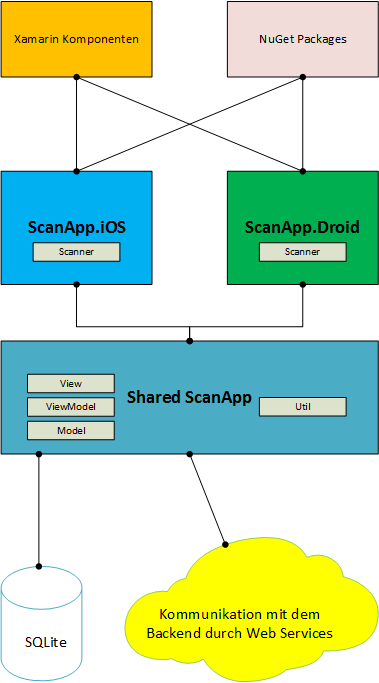
\includegraphics[scale = 0.7]{graphics/ScanApp_Projekt.png}
\caption{ScanApp - Entwurf}
\label{fig:abb40}
\end{figure}
Abb. \ref{fig:abb40} veranschaulicht die Verteilung der Projekten.
Der Gro�teil des Codes wird sich im plattform�bergreifenden Projekt, ScanApp befinden. In diesem
"`shared"' Projekt wird typischerweise die gesamte App-Logik, inklusive Gestaltung der
Benutzungsoberfl�che, ausgelagert. 
% Xamarin.Forms ist eine Art Abstraktionsschicht, mit derer Hilfe
% sich die Benutzungsoberfl�che in diesem gemeinsamen, plattform�bergreifenden Projekt gestalten
% l�sst.
Die Benutzungsoberfl�che (in English: graphical user interface (GUI)) soll den Designvorgaben der
unterschiedlichen Betriebssystemhersteller folgen, damit die App zu den entsprechenden App-Stores
zugelassen wird.
Der Entwickler soll sich, allerdings, nicht darum k�mmern, diese Aufgabe erledigt Xamarin. Da der Xamarin-Code pro Plattform zu Maschinencode
kompiliert wird, ist der App nicht anzusehen, dass die "`cross-plattform"' entwickelt wurde.
Aus der Perspektive eines Benutzers f�hlt sich eine Xamarin.iOS App wie jede native iOS App an und
jede Xamarin.Android App.wie eine nativ entwickelte Android App. 
Dank Xamarin.Forms werden die Ansichten komplett plattformunabh�ngig definiert. 
Die Xamarin.Forms Steuerelemente werden je nach Plattform in das native Pendant �bersetzt.
So wird ein "`Xamarin.Forms.ListView"' in "`ListView"' bei Android und in "`UITableView"' bei iOS �bersetzt
\\In die
Projekte ScanApp.Droid und ScanApp.iOS geh�ren App-Ressourcen wie bspw.
Icons, sowie eventuell benutzerdefinierte Renderer. Die sogenannten "`Custom Renderer"' werden f�r
die Implementierung von benutzerdefinierten Steuerelementen und Ansichten ben�tigt, die mit den von
Xamarin.Forms zur Verf�gung gestellten Werkzeugen nicht zu realisieren sind.
\\Au�er als Container f�r benutzerdefinierte Renderer und App-Ressourcen, werden in den
plattformspezifischen Projekte noch Einstellungen vorgenommen, wie Info.plist im iOS-Projekt oder
AndroidManifest.xml bei Android. 
Wie aus Abb. \ref{fig:abb40} ersichtlich, lassen sich beim "`Shared Projects"'-Ansatz keine "`open
source"' Bibliotheken, wie NuGet Packages oder Xamarin Komponenten direkt an das gemeinsame Projekt anbinden.
Das erfolgt in den plattformspezifischen Projekte. Eine solche Xamarin Komponente ist bspw. die ZXing-Komponente zum Scannen von Barcodes, die
eine zentrale Rolle in der App spielt. Das ebenso in der ScanApp eingebundene NuGet Package
"`DeviceInfo"' bietet eine API, mit der Entwickler Informationen �ber das Smartphone bekommen
k�nnen. Am Ende dieses Kapitels werden die f�r die ScanApp ben�tigten NuGut Packages und Xamarin
Komponenten n�her vorgestellt. 
% \\Der Entwurf der ScanApp bezieht sich fast ausschlie�lich auf das
% "`shared"' Projekt (siehe Abb. \ref{fig:abb40}). 
\\Wie bereits angesprochen, wird mit
"`Cross-Plattform-Entwicklung"' gezielt, dass alles, was sich auslagern l�sst, in das gemeinsame
Projekt geh�rt. Die plattformspezifischen Projekte sollten m�glichst "`leer"' bleiben.
Im Folgenden wird einen Einblick in die Strukturen der drei Projekte gegeben, beginnend beim
"`shared"' ScanApp Projekt (siehe Abb. \ref{fig:abb41}).
\begin{figure}[!h]
\centering
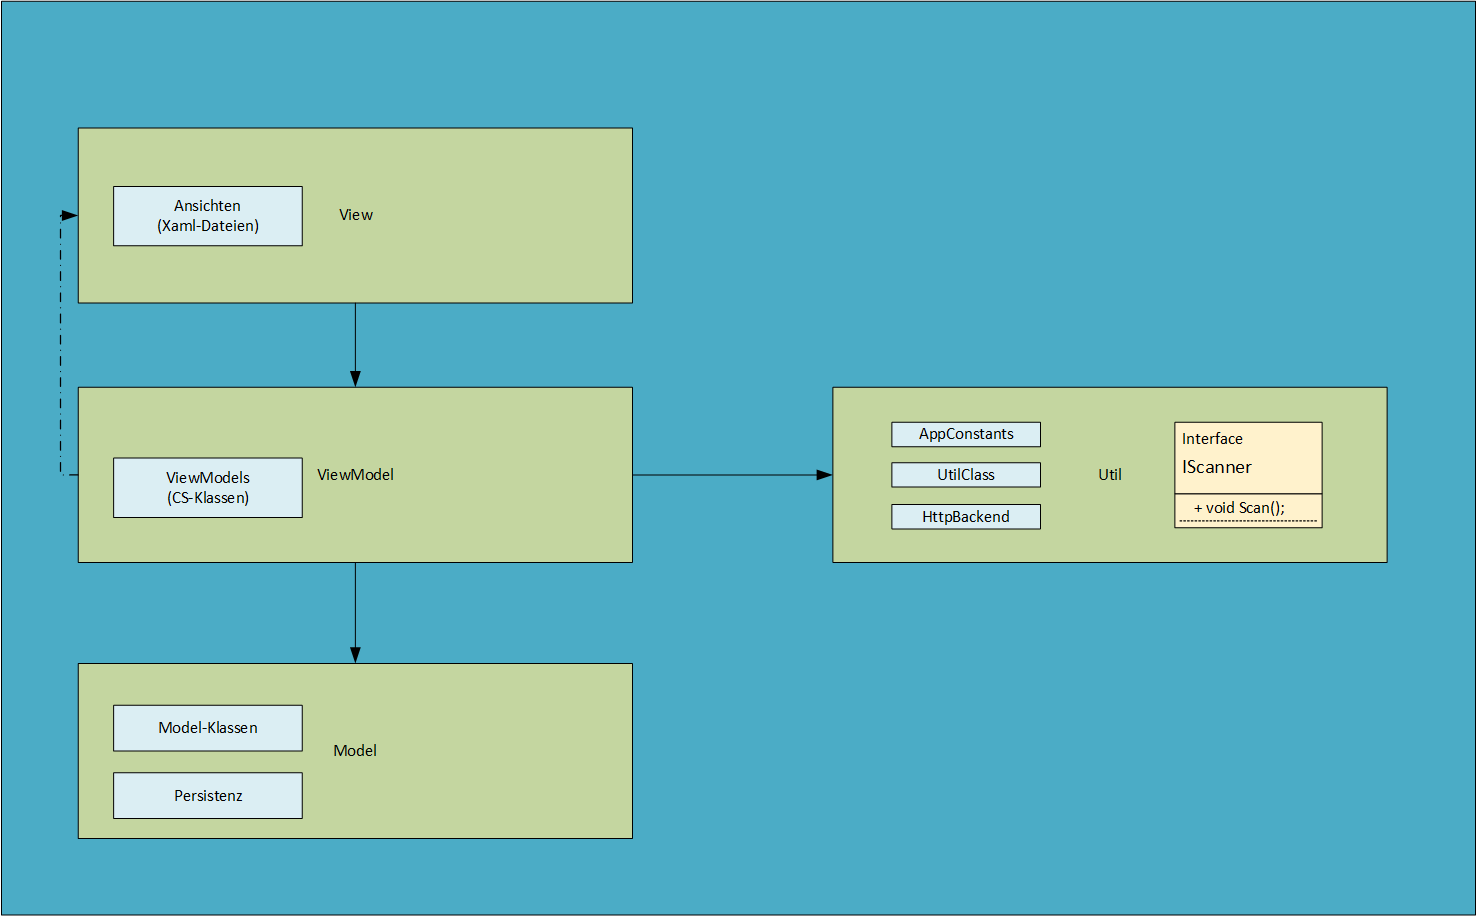
\includegraphics[scale = 0.46]{graphics/SharedScanApp.png}
\caption{ScanApp - Entwurf (Shared Projekt)}
\label{fig:abb41}
\end{figure}
% \\Sollte eine
% Anforderung nicht plattform�bergreifend zu gew�hrleisten sein, muss diese Funktionalit�t in den
% plattformspezifischen Projekten implementiert werden. Im gemeinsamen Projekt wird ein Interface
% definiert, das von den daf�r zust�ndigen Klassen in ScanApp.Droid und ScanApp.iOS implementiert
% werden muss.
% Die angeforderte Funktionalit�t wird in den plattformspezifischen Projekten implementiert. Dieses
% Interface muss von den jeweiligen Klassen, die die Funktionalit�t gew�hrleisten, der plattformspezifischen Projekte implementiert.
% Der Zugriff aus dem plattform�bergreifenden Projekt erfolgt folgenderma�en:\\
% \textcolor{gray}{\emph{DependencyService.Get<InterfaceName>().PlattformSpecificMethodName()}}.
% \subsection{Umsetzung des MVVM-Architekturmusters}
% Wie bereits im Kapitel \ref{MVVM} er�rtert, weist das MVVM-Pattern eine lose Kopplung
% zwischen View und Viewmodel auf. Um diese Trennung visuell zu gestalten, werden drei Ordner erstellt:
% \begin{itemize}
%   \item \textbf{Model} - Im Ordner Model werden typischerweise Klassen defniert, die
%   anwendungsspezifische Datentypen beschreiben. Das sind Klassen zur Speicherung und
%   Verarbeitung von Daten, die daf�r sorgen, dass die Daten konsistent gehalten
%   werden.
%   \item \textbf{View} - Alle Ansichten (Xaml-Datein, die vom Typ Xamarin.Forms.Page oder
% Xamarin.Forms.View sind oder von diesen Klassen erben) geh�ren in den Ordner View.
%   \item \textbf{Viewmodel} - In den Viewmodel-Ordner kommen die Viewmodel-Klassen (C\#-Klassen,
%   die das Interface \textbf{\textit{INotifyPropertChanged}} implementieren). 
% \end{itemize}
% Jede Ansicht wird an ein Viewmodel gebunden. Das wird durch das sogenannte "`Data
% Binding"' (in Deutsch Datenbindung) realisiert.
% % In Abb.\ref{fig:abb23} sieht man eine typische
% % Xaml-Datei, die eine Ansicht beschreibt und sich im Ordner View befindet. Diese Ansicht wird
% % von der benutzerdefinierten Base\_Page abgeleitet, die ihrerseits von der Klasse Xamarin.Forms.Page
% % abgeleitet wird.
%  In einer C\#-Klasse, genannt Base\_Page, werden Eigenschaften und Methoden definiert, die f�r die
%  meisten Ansichten gemeinsam sind. Bspw. das Navigationsheader-Logo oder Methoden f�r die Steuerung
% der Navigation. Diese Klasse wird von der Klasse Xamarin.Forms.Page abgeleitet.
% % \\Eine der wichtigsten Klassenvariablen der Klasse Xamarin.Forms.Page ist das Property
% % \textit{BindingContext}.
% % Mithilfe dieser Eigenschaft wird ein Viewmodel (in diesem Fall das HeaderDataEditViewModel) an der Page-Klasse gebunden (Siehe
% % \ref{fig:abb23}, Zeile 23-25).
% % \\In Zeile 12 findet eine typische Datenbindung ("`data binding"') statt.
% % Das Text-Property eines Entry-Textfeldes wird an das Property \textit{Name} gebunden, das im
% % Viewmodel definiert wird (siehe Abb.\ref{fig:abb33}).
% % Sobald der Text des Textfelds sich �ndert, wird das Viewmodel dar�ber informiert. Diese Bindung
% % funktioniert in beiden Richtungen, d.h. �nderungen, die im Viewmodel vorgenommen werden, werden in
% % der Ansicht angezeigt.\\In Abbildung \ref{fig:abb23}, Zeile 20 ist die Definition eines
% % Toolbarbuttons zu sehen. Sobald dieser Button gedr�ckt wird, wird ein Command ausgef�hrt, das an
% % das Property \textit{SaveUserDataCommand} des Viewmodels gebunden ist. D.h. dieses Klick-Event
% % l�st den Aufruf einer Methode in der Viewmodel-Klasse auf.\\Das Ganze veranschaulicht, welche
% % Vorteile das MVVM-Architekturmuster mit sich bringt.
% Durch die Datenbindung entsteht eine lose Kopplung zwischen View und ViewModel. Da das Viewmodel die
% Views nicht kennt, l�sst sich eine Ansicht problemlos durch eine andere austauschen. Die neue
% Ansicht muss lediglich an das Viewmodel gebunden werden.
% \\Ein ViewModel muss zwingend das Interface \textbf{\textit{INotifyPropertChanged}} implementieren.
% Dadurch k�nnen sogenannte "`Bindable Properties"` definiert werden
% %  (siehe Abb.\ref{fig:abb33})
% . Bei jeder �nderung wird die OnPropertyChanged()-Methode mit dem Property-Name als String-Parameter
% aufgerufen und dadurch wird ein PropertyChangedEventHandler ausgel�st.
% \\Wie bei den meisten Applikationen, sind auch f�r die Scan-Anwendung mehrere Ansichten
% erforderlich. Es stellt sich die Frage, wie wird zwischen den verschiedenen Seiten gewechselt?\\Um
% zwischen den Ansichten navigieren zu k�nnen, wird eine Instanz der Klasse \textit{NavigationPage}
% ben�tigt: \textit{new NavigationPage(new Page())}. 
% \\Jede Xamarin.Forms.Page-Klasse hat �ber das Property \textbf{\textit{Navigation}} Zugriff auf das
% NavigationPage: \textit{this.Navigation.PushAsync(new Page())}.\\Nach dem MVVM-Muster sollten sich
% die Viewmodel-Klassen um die Navigation k�mmern.
% Allerdings ist \textit{Navigation} ein Property der Ansicht. D.h. das Viewmodel muss signalisieren,
% dass es zu einer anderen Ansicht gewechselt werden soll. Da das Viewmodel die Ansicht nicht kennt,
% kann das durch das \textbf{\textit{Xamarin.Forms Messaging Center}} erreicht werden. Die Ansicht
% abonniert Navigationsnachrichten des Viewmodels und wird somit immer informiert, wenn die
% Seite gewechselt werden soll.

% \begin{itemize}
%   \item Das Framework MVVM-Light
%   \item Messaging
%   \item unsaubere Anwendung von MVVM, wie z.B. das Property NavigatioPage einer Ansicht dem
%   zugeh�rigen ViewModel mitzugeben. Das w�rde die Navigation aus dem ViewModel erm�glichen, aber
%   es verletzt eine der Grundideen von MVVM ist es, dass der ViewModel die View nicht kennt.
% \end{itemize}


% \begin{figure}[!h]
% \centering
% 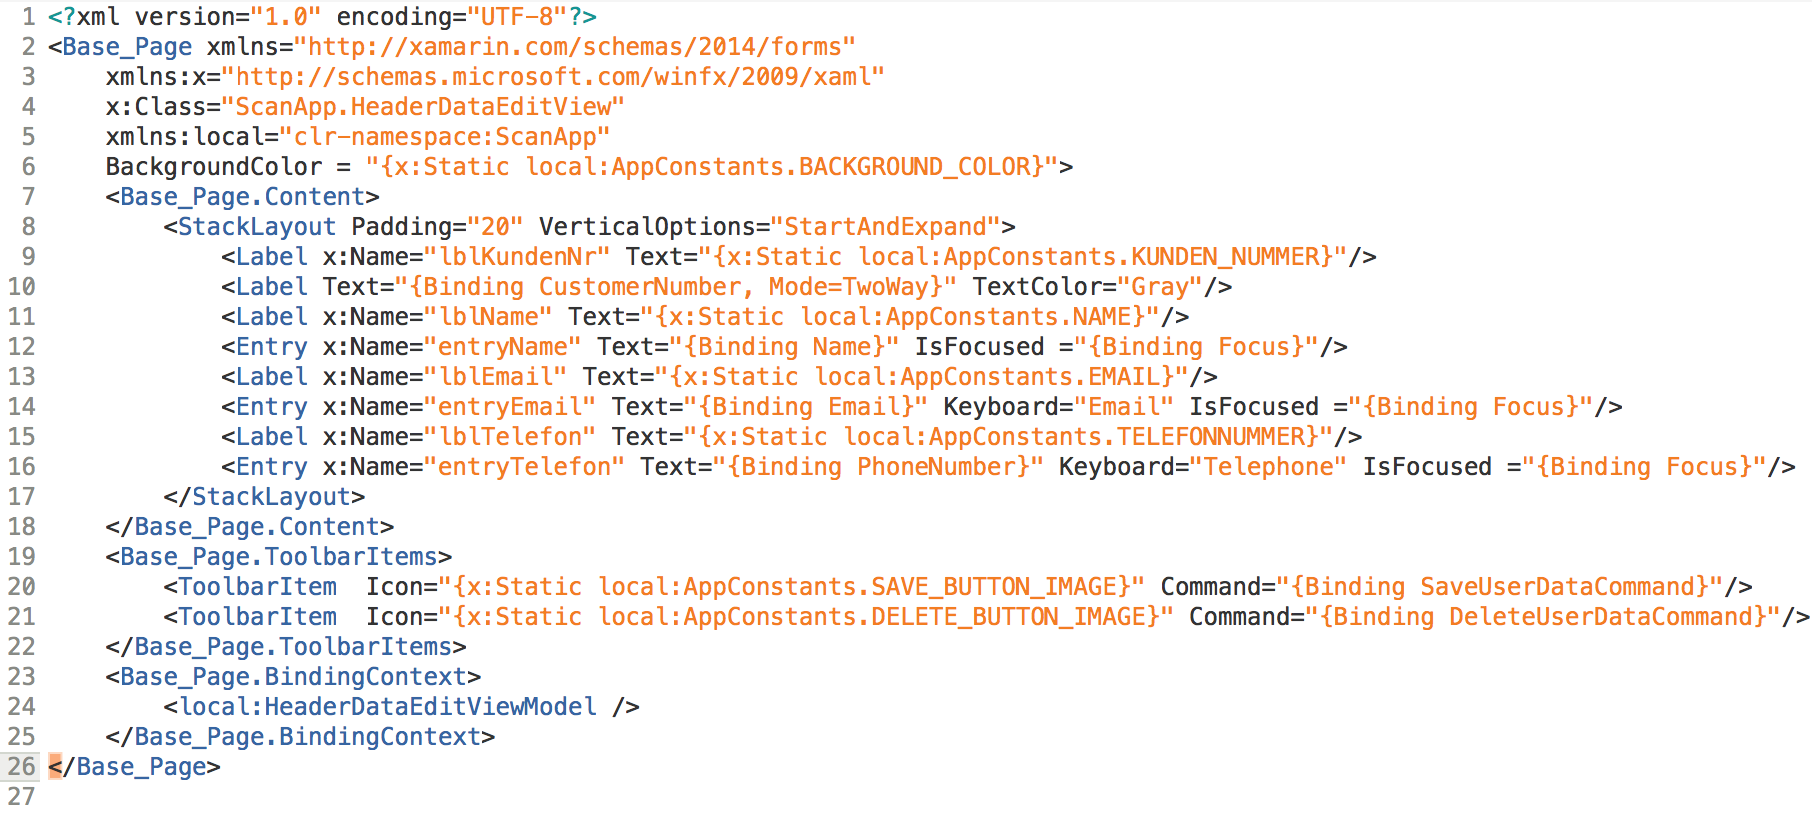
\includegraphics[scale = 0.435]{graphics/Typische_Xaml_Datei.png}
% \caption{Typische Xaml-Datei}
% \label{fig:abb23}
% \end{figure}
% \begin{figure}[!h]
% \centering
% 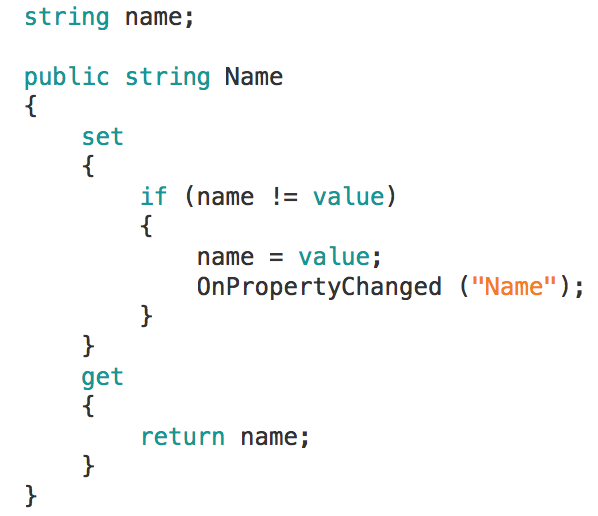
\includegraphics[scale = 0.6]{graphics/Bindable_Property.png}
% \caption{Definition von Bindable Property}
% \label{fig:abb33}
% \end{figure}

% Da beim gemeinsamen ScanApp Projekt keine Bibliotheken eingebunden werden k�nnen, muss man einen
% SQLite.cs File aus Github herunterladen und in das gemeinsame Projekt kopieren. Dieser C\#-File
% benutzt Compiler Direktiven um mehrere Plattformen in derselben Codebasis zu unterst�tzen.
% \\Um SQLite in einer Xamarin.iOS oder Android Applikation benutzen zu k�nnen, muss man angeben, wo
% der Datenbank File zu finden ist (es ist abh�ngig vom
% Ziel-Plattform unterschiedlich). F�r iOs und Android kann man "`Environment class"' benutzen um einen
% validen Pfad zu konstruieren (siehe Abb. \ref{fig:abb27}). Mittels Compiler Direktiven lassen sich
% spezielle Pfade f�r jede Plattform generieren.\\Um sicher zu gehen, dass der Code nicht versucht,
% auf die SQLite Datenbank aus verschiedenen "`multiple Threads"' zuzugreifen wird manuel ein "`lock"'
% benutzt. Z.B.\\object locker = new object();\\lock(locker)\{ Datenbankquery \};\\Alle
% Datenbankzugriffe sind mit demselben "`lock"' gekapselt, wobei hier Vorsicht geboten ist. Es k�nnten
% Deadlocks entstehen! 
% \begin{figure}[!h]
% \centering
% 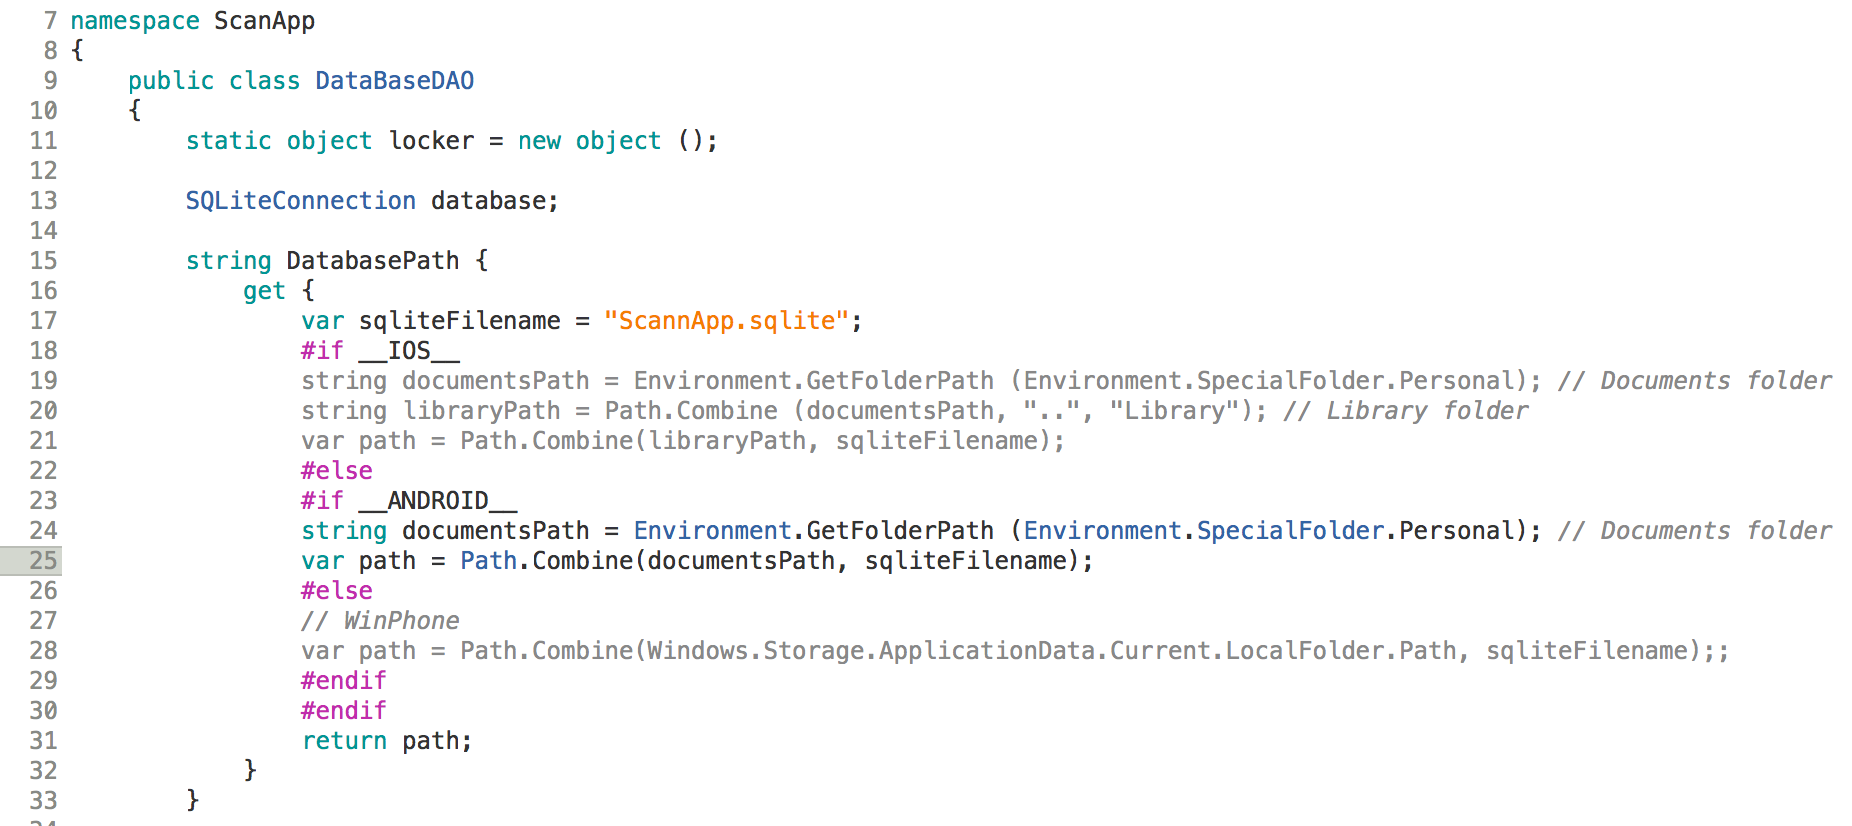
\includegraphics[scale = 0.4]{graphics/SQLitePath.png}
% \caption{SQLite Pfad}
% \label{fig:abb27}
% \end{figure}
\section{Shared ScanApp Projekt}
In Abb. \ref{fig:abb40} wird der grobe Entwurf der ScanApp abgebildet. Wie schon angemerkt, passiert
das wesentliche im gemeinsamen Projekt (Shared Projekt). Abb. \ref{fig:abb41} bildet die Struktur
des Shared ScanApp Projekts ab. Im Folgenden wird einen Einblick in die Komponenten dieses Projekts
gegeben. Wie bereits im Kapitel \ref{MVVM} er�rtert, weist das MVVM-Pattern eine lose Kopplung
zwischen View und Viewmodel auf. Um diese Trennung visuell zu gestalten, werden drei Ordner erstellt:
\subsection{Model}
In der Komponente Model werden typischerweise Klassen definiert, die
  anwendungsspezifische Datentypen beschreiben. Das sind Klassen zur Speicherung und
  Verarbeitung von Daten, die daf�r sorgen, dass die Daten konsistent gehalten
  werden.
D.h. zum Model geh�ren die eigentlichen Daten der Anwendung. Hier werden Klassen, wie Barcode,
UserData, Order, OrderItem etc. definiert.\\Im Model wird noch eine Klasse definiert, die
Methoden f�r "`CRUD"'-Operationen (Create Read Update Delete) f�r das Persistieren der Modeldaten in
die Datenbank bietet, die in \ref{PersistenzBackend} vorgestellt wird.
\subsection{View}\label{View}
In der View-Komponente werden die Ansichten der Bedienungsoberfl�che der App definiert. 
Die grafischen Interfaces der Scan-App werden mit der Markupsprache Xaml
beschrieben. Somit wird eine strikte Trennung zwischen dem Oberfl�chendesign (in einer
Xaml-Datei beschrieben) und der Funktionalit�t (in einer an der Xaml-Datei gebundenen C\#-Datei aus
der Komponente ViewModel implementiert) erreicht.
\\An dieser Stelle l�sst es sich anmerken, dass Xamarin Entwicklern die Wahl zwischen der
Markupsprache Xaml und C\# f�r die Implementierung der UIs (User Interfaces) l�sst, wobei beide
Techniken zum gleichen Ergebnis f�hren. D.h. die Verwendung von Xaml f�r die Beschreibung der
Benutzungsoberfl�che ist kein Pflicht, allerdings ist der C\#-Code schwerer lesbar als der
Xaml-Code. Aus diesem Grund wird f�r die vorliegende Arbeit die Xaml-Technik angewendet.
% \\Aus diesem Grund werden die grafischen Interfaces der Scan-App mit der Markupsprache Xaml
% beschrieben. Somit wird eine strikte Trennung zwischen dem Oberfl�chendesign (in einer
% Xaml-Datei beschrieben) und der Funktionalit�t (in der an der Xaml-Datei gebundenen
% Viewmodel-C\#-Datei implementiert) erreicht.
Dieser Ansatz macht Wiederverwendbarkeit und Austauschbarkeit einer Ansicht m�glich und Designer und
Entwickler k�nnen unabh�ngig voneinander arbeiten.
% In Abb. \ref{fig:abb34} werden die Mockups f�r die unterschiedelichen Ansichten der Scan-App
% abgebildet.
In Abb. \ref{fig:abb34} werden Mockups der zu definierenden Scan-App Ansichten dargestellt.
Jede Ansicht wird in Form einer Xamarin.Forms.Page definiert und in einer Xaml-Datei gespeichert. 
In einer C\#-Klasse, genannt Base\_Page, die von der Klasse Xamarin.Forms.Page abgeleitet wird,
werden Eigenschaften definiert, die f�r die meisten Ansichten gemeinsam sind. Bspw. das
Navigationsheader-Logo oder Methoden f�r die Steuerung der Navigation. Von dieser Klasse werden die
Ansichten abgeleitet.
\begin{figure}[!h]
\centering
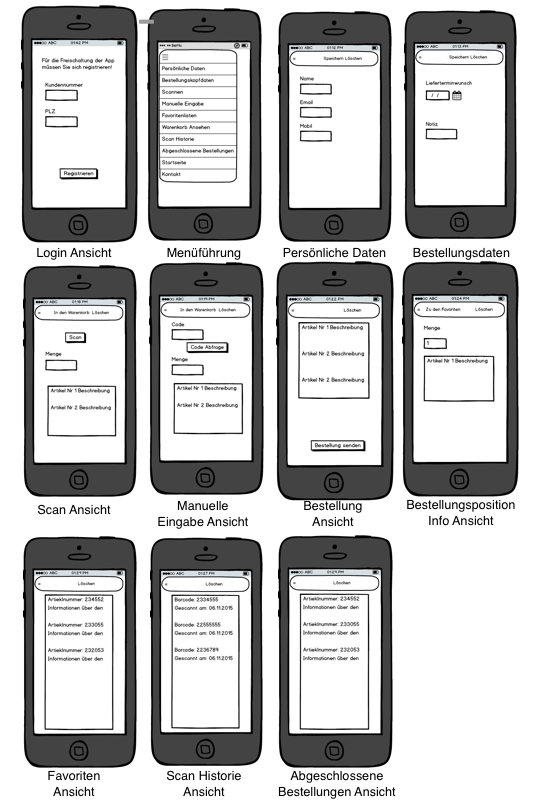
\includegraphics[scale = 0.65]{graphics/MockUpsScanApp.png}
\caption{GUI Mockups}
\label{fig:abb34}
\end{figure}
\subsection{ViewModel}
In der Viewmodel-Komponente kommen die Viewmodel-Klassen (C\#-Klassen, die das Interface
\textbf{\textit{INotifyPropertChanged}} implementieren). Jede der in der Komponente View definierten
Ansichten, wird an eine ViewModel-Klasse gebunden. W�hrend eine Xaml-Datei, eine reine
Beschreibung der Ansicht ist, wird in einer ViewModel-Klasse die Logik hinter dieser Ansicht
implementiert. Hier werden Properties und Methoden definiert, die durch "`Data Binding"' an
Steuerelemente des dazugeh�renden Views gebunden werden. \\Die Klassen der ViewModel-Komponente
greifen auf die Klassen der Util- und der Model-Komponente zu, um die Funktionalit�t der App zu
gew�hrleisten und sind auch f�r die Navigation zwischen der App-Seiten, die im
\ref{Navigation} beschrieben wird, zust�ndig. Da nach MVVM die View den ViewModel kennt, nicht aber
andersrum, kann eine ViewModel-Klasse ausschlie�lich durch das \textbf{\textit{Xamarin.Forms Messaging Center}} mit der entsprechende View-Klasse
"`kommunizieren"'.
\subsection{Util}
In dieser Komponente werden einige n�tzliche Klassen definiert: 
\begin{itemize}
  \item UtilKlasse mit mehreren statischen Methoden, die von den Klassen des Viewmodels benutzt
  werden.
  \item Klasse mit App-Konstanten. Hier werden �blicherweise vorwiegend Strings ausgelagert.
  \item HttpBackend. Diese Klasse kapselt die Kommunikation mit dem Backend mittles Web Services.
\end{itemize}

Es ist m�glich, dass die Funktionalit�t eines Viewmodels in der Code-Behind-Datei einer Ansicht
untergebracht wird (Beim Erstellen einer Xaml-Datei wird automatisch auch die dazugeh�rende
C\#-Code-Behind-Datei erstellt).
Das entspricht, allerdings, nicht dem MVVM-Architekturmuster.
Dadurch w�rde eine sehr enge Kopplung zwischen View und Funktionalit�t entstehen und die Ansichten w�ren
nicht mehr austauschbar.\\Durch Xamarin.Forms kann man die ganze Benutzungsoberfl�che im gemeinsamen
Projekt implementieren. D.h. jede Erweiterung oder �nderung einer Ansicht kann zentral, an einer
Stelle, durchgef�hrt werden. Sollte man zu einem sp�teren Zeitpunkt Design-�nderungen vornehmen
m�chten, m�sste man es dann nur einmal implementieren.\\Da der gemeinsame Code zu nativem
Maschinencode kompiliert wird und die Steuerelemente die gleiche Funktionalit�t haben, sieht die
Android-Benutzungsoberfl�che nicht unbedingt gleich wie die von iOS oder eventuell die von Windows
Phone aus.\\Ein Eingriff in die plattformspezifischen Projekte, ist nur in den F�llen notwendig,
wenn die von Xamarin.Forms angebotenen Steuerelemente sich nicht so verhalten wie der Entwickler bzw. der Designer der App es sich vorstellt. Dann werden sogenannte
"`Custom Renderer"' Klassen in die plattformspezifischen Projekten ben�tigt. In denen kann man
�nderungen vornehmen, wie z.B. das Definieren von runden Buttons. \\Die Layouts der  mit
Xamarin.Forms erstellten Ansichten passen sich dynamisch an die Gr��e des Bildschirms an.
Bei den vielen verschiedenen Ger�ten ist das eine wesentliche Erleichterung f�r den Entwickler.
\section{Datenpersistenz und Backend-Kommunikation}\label{PersistenzBackend}
Fast jede mobile Anwendung braucht einen Mechanismus, der eine dauerhafte lokale Speicherung der
Appdaten erlaubt. Das gilt besonders f�r die Kategorie der Business Apps, zu der die zu entwickelnde
ScanApp auch z�hlt. Typischerweise wird zu diesem Zweck eine leichtgewichtige Datenbank, namens
SQLite benutzt.
Die "`open-source"' Datenbank SQLite ist gut geeignet f�r das Persistieren von Daten von mobilen
Applikationen, weil:
\begin{itemize}
  \item die Datenbank klein, schnell und leicht portierbar ist;
  \item der Fileformat leicht zu benutzen und plattform�bergreifend ist;
  \item SQLite die meisten SQL92 Standards implementiert.
\end{itemize}
Dar�ber hinaus ist SQLite die Standardl�sung bei der nativen Android-App-Entwicklung und sehr
verbreitet bei der iOS-App-Entwicklung.
Xamarin.Forms unterst�tzt die Anbindung von SQLite und zwar cross-plattform. In den plattformspezifischen Projekte
muss lediglich jeweils eine SQLite-Datei zu den Ressourcen hinzugef�gt werden. Im gemeinsamen
Projekt muss der Pfad zu der SQLite-Datenbank angegeben werden, einmal f�r Android und
einmal f�r iOS. Die Zugriffe auf die Datenbank erfolgen plattform�bergreifend (d.h. aus dem
"`shared"' Projekt).

Ein weiterer wichtiger und h�ufig vorkommender Punkt bei der Entwicklung von Apps, ist die
Kommunikation mit dem Backend. �hnlich wie die Anforderung f�r dauerhafte lokale Speicherung der App
Daten, m�ssen viele Apps (vor allem Business Apps) mit einem Server �ber das Internet kommunizieren.
Diese Kommunikation erfolgt �ber sogenannte Web Services.
\\Stellvertretend f�r die meisten Apps dieser Kategorie, kommt es bei der ScanApp in den
folgenden F�llen zum Einsatz von Web Services:
\begin{itemize}
  \item Bei der einmaligen Registrierung eines Benutzers.
  \item Beim �berpr�fen eines Barcodes.
  \item Beim Abschlie�en einer Bestellung.
\end{itemize} 
Das sind drei typische Interaktionen zwischen App und Backend. Im Prinzip ist es belanglos,
wof�r konkret Web Services eingesetzt werden, weil die immer nach dem gleichen Muster funktionieren.
Die App sendet eine Anfrage, im vorliegenden Fall in Form eines Json-Objekts (oft werden auch XML-Dateien zwischen App
und Server ausgetauscht, wobei bei XML der Overhead gr��er ist) und der Server antwortet
mit einer Datei desselben Formats. Damit die Kommunikation gelingt, m�ssen sich Server und Client an
einem Vertrag halten. In diesem Vertrag wird die Struktur des Json-Objekts definiert. D.h.
die App muss in der Lage sein, dieses Objekt zu zerteilen (parsen), um die Antwort vom Server
verstehen zu k�nnen. F�r das Parsen eines Json-Objekts wird das NuGet Package \textbf{Newtonsoft.Json} in 
die Projekte ScanApp.iOS und ScanApp.Droid eingebunden. Die Kommunikation erfolgt mit dem
Http-Client der Xamarin Komponente \textbf{ModernHttpClient}, die ebenso in die
plattformspezifischen Projekte eingebunden werden muss.\\Die Implementierung ist allerdings
plattform�bergreifend. Im gemeinsamen Projekt wird eine Klasse (siehe Abb. \ref{fig:abb41}, die
Klassse HttpBackend in der Util-Komponente) mit jeweils eine Methode f�r die oben genannten drei
F�llen erstellt.
% \\  
% \textcolor{gray}{\emph{HttpClient client = new HttpClient(new
% ModernHttpClient.NativeMessageHandler())}}.
\\Wie bei jeder App muss man hier beachten, dass mobile Ger�te nicht selten einen schlechten oder
gar keinen Empfang haben. Abh�ngig vom Netzwerktyp kann die Geschwindigkeit einer Internetverbindung
stark variieren. Aus diesem Grund ist es wichtig, dass alle Serveranfragen in einem
separaten Thread ausgef�hrt werden, so dass der Ablauf der App nicht durch eine schlechte oder
fehlende Verbindung beeintr�chtigt wird. Au�erdem kann je nach Tarif der mobile Datenvolumen
begrenzt oder es k�nnen extra Kosten entstehen, wenn eine Bestimmte Grenze von verbrauchten MB pro Monat erreicht
wird. Aus diesem Grund ist es sinnvoll, dass die App in der Lage ist, den Netzwerktyp zu
erkennen. D.h. ob die Verbindung �ber WLAN oder �ber das mobile Internet erfolgt. Xamarin.Android
bietet einen Mechanismus f�r diesen Zweck - durch die Klasse \textbf{NetworkInfo}. Mithilfe dieser Klasse
kann die App auch erkennen ob Roaming eingeschaltet wurde (\cite{XamNetzwerkStatus}).\\Bei
Xamarin.iOS gibt es einen �hnlichen Mechanismus.
\\Der Befehl \textcolor{gray}{\textsl{Reachability.InternetConectionStatus()}} liefert Auskunft
dar�ber ob eine Internetverbindung �ber WLAN, �ber mobiles Internet erfolgt oder es gar keine
Verbindung besteht (\cite{XamNetzwerkStatusIOS}). \\Die Netzwerktyperkennung l�sst sich nicht
plattform�bergreifend implementieren, das erfolgt in den plattformspezifischen Projekten. Im Sinne von "`Cross-Plattform-Entwicklung"' wird f�r solche F�lle ein Interface im gemeinsamen Projekt definiert. Dieses Interface wird dann in den plattformspezifischen Projekten implementiert. Auf
diese Weise l�sst sich die Netzwerktyperkennung aus dem "`shared"' Projekt steuern und
dementsprechend behandeln. Da bei der ScanApp eine �bertragung von
gr��eren Dateien, wie bspw. Bilder nicht vorgesehen ist, ist eine Netzwerktyperkennung unn�tig und
es wurde darauf verzichtet.

% Die Benutzungsoberfl�che (in English: graphical user interface (GUI)) soll den Designvorgaben der
% unterschiedlichen Betriebssystemhersteller folgen. Der Entwickler soll sich, allerdings, nicht darum
% k�mmern, diese Aufgabe erledigt Xamarin. Der Xamarin-Code wird pro Plattform zu Maschinencode
% kompiliert und dadurch erweckt die App den Eindruck, Teil der konkreten Plattform zu sein. D.h.
% aus der Perspektive eines Benutzers f�hlt sich eine Xamarin.iOS App wie jede native iOS App an.
% Selbstverst�ndlich gilt dasselbe f�r eine Xamarin.Android App. \\In Abb.
% \ref{fig:abb34} werden die Mockups f�r die unterschiedelichen Ansichten der Scan-App abgebildet. 
% Die GUI wird mit wenigen Ausnahmen im gemeinsamen Projekt, ScanApp erstellt.
% Xamarin l�sst Entwicklern die Wahl zwischen der Markupsprache Xaml und C\# f�r die Implementierung
% der UIs (User Interfaces), wobei beide Techniken zum gleichen Ergebnis f�hren. \\Die
% Positionierung der Steuerelemente und deren Funktionalit�t lassen sich in einer C\#-Datei
% implementieren, allerdings ist der Code schwer lesbar und nicht wiederverwendbar.\\Aus diesem
% Grund werden die grafischen Interfaces der Scan-App mit der Markupsprache Xaml beschrieben.
% Somit wird eine strikte Trennung zwischen dem Oberfl�chendesign (in einer
% Xaml-Datei beschrieben) und der Funktionalit�t (in der an der Xaml-Datei gebundenen
% Viewmodel-C\#-Datei implementiert) erreicht.
% Diese Technik macht Wiederverwendbarkeit und Austauschbarkeit einer Ansicht m�glich und Designer und
% Entwickler k�nnen unabh�ngig voneinander arbeiten. \\Bei der Erstellung einer Xamarin.Forms
% ContentPage Xaml-Datei wird automatisch auch die zugrundeliegende C\#-Datei, bekannt auch als "`Code-Behind-Datei"', angelegt (siehe Abb. \ref{fig:abb21}).
% Diese Code-Behind-Datei sollte bei einer sauberen Umsetzung des MVVM-Patterns au�er des Aufrufs der
% \emph{InitializeComponent()} Methode im Konstruktor und der bereits erw�hnten Methoden, die
% Viewmodelnachrichten abonnieren und die Navigation steuern, komplett leer sein.
% Es ist m�glich, dass die Funktionalit�t eines Viewmodels in der Code-Behind-Datei einer Ansicht
% untergebracht wird. Das entspricht, allerdings, nicht dem MVVM-Architekturmuster. Dadurch
% w�rde eine sehr enge Kopplung zwischen View und Funktionalit�t entstehen und die Ansichten w�ren
% nicht mehr austauschbar.\\Durch Xamarin.Forms kann man die ganze Benutzungsoberfl�che im gemeinsamen
% Projekt implementieren. D.h. jede Erweiterung oder �nderung einer Ansicht kann zentral, an einer
% Stelle, durchgef�hrt werden. Sollte man zu einem sp�teren Zeitpunkt Design-�nderungen vornehmen
% m�chten, m�sste man es dann nur einmal implementieren.\\Da der gemeinsame Code zu nativem
% Maschinencode kompiliert wird und die Steuerelemente die gleiche Funktionalit�t haben, sieht die
% Android-Benutzungsoberfl�che nicht unbedingt gleich wie die von iOS oder eventuell die von Windows
% Phone aus.\\Ein Eingriff in die plattformspezifischen Projekte, ist nur in den F�llen notwendig,
% wenn die von Xamarin.Forms angebotenen Steuerelemente sich nicht so verhalten wie der Entwickler bzw. der Designer der App es sich vorstellt. Dann werden sogenannte
% "`Custom Renderer"' Klassen in die plattformspezifischen Projekten ben�tigt. In denen kann man
% �nderungen vornehmen, wie z.B. das Definieren von runden Buttons. \\Die Layouts der  mit
% Xamarin.Forms erstellten Ansichten passen sich dynamisch an die Gr��e des Bildschirms an.
% Bei den vielen verschiedenen Ger�ten ist das eine wesentliche Erleichterung f�r den Entwickler. 
% \begin{figure}[!h]
% \centering
% 
\includegraphics[scale = 0.7]{graphics/XamlDateiPlusCSDatei.png}
% \caption{Xaml-Datei und die zugrundeliegende C\#-Datei}
% \label{fig:abb21}
% \end{figure}
% 
% \begin{figure}[!h]
% \centering
% 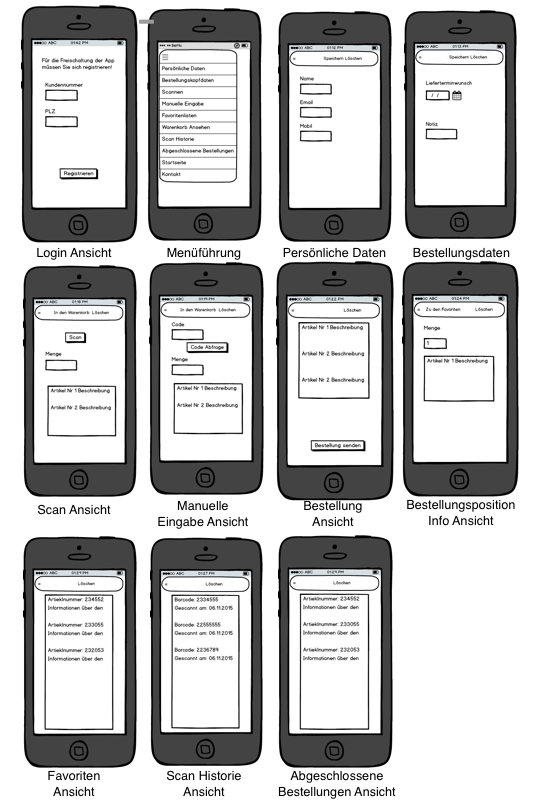
\includegraphics[scale = 0.65]{graphics/MockUpsScanApp.png}
% \caption{GUI Mockups}
% \label{fig:abb34}
% \end{figure}
% \\Der Aufbau einer Xaml-Datei ist dem Ger�st eines XML-Dokuments sehr �hnlich. Es gibt ein
% Wurzelelement und jedes Element kann Attribute besitzen. Dadurch entsteht eine �bersichtliche Hierarchie der Elemente
% (Siehe \ref{fig:abb23}).
% Durch das Attribut x:Name k�nnte man auf das Element aus der Code-Behind-Datei zugreifen und bspw. den
% Text eines Labels oder die Textfarbe setzen. 
% (siehe \ref{fig:abb26}).

% \\In Abbildung \ref{fig:abb25} sieht man die zugrundeliegenden C\#-Datei, in der z.B. die
% Funktionalit�t der Toolbar-Buttons implementiert ist. Beim Klick auf den Button zum Speichern der
% Angaben, werden die Texten der Texteingabefeldern in einem Objekt vom Typ Kopfdaten gespeichert und
% anschlie�end wird das neu erstellte Objekt in die SQLite-Datenbank gespeichert. Beim Klick auf den
% M�llkorb-Button, werden die gespeicherten pers�nlichen Daten aus der SQLite-Datenbank gel�scht. 
% \begin{figure}[!h]
% \centering
% 
\includegraphics[scale = 0.7]{graphics/XamlDateiPlusCSDatei.png}
% \caption{Xaml-Datei und die zugrundeliegende C\#-Datei}
% \label{fig:abb21}
% \end{figure}
% \begin{figure}[!h]
% \centering
% 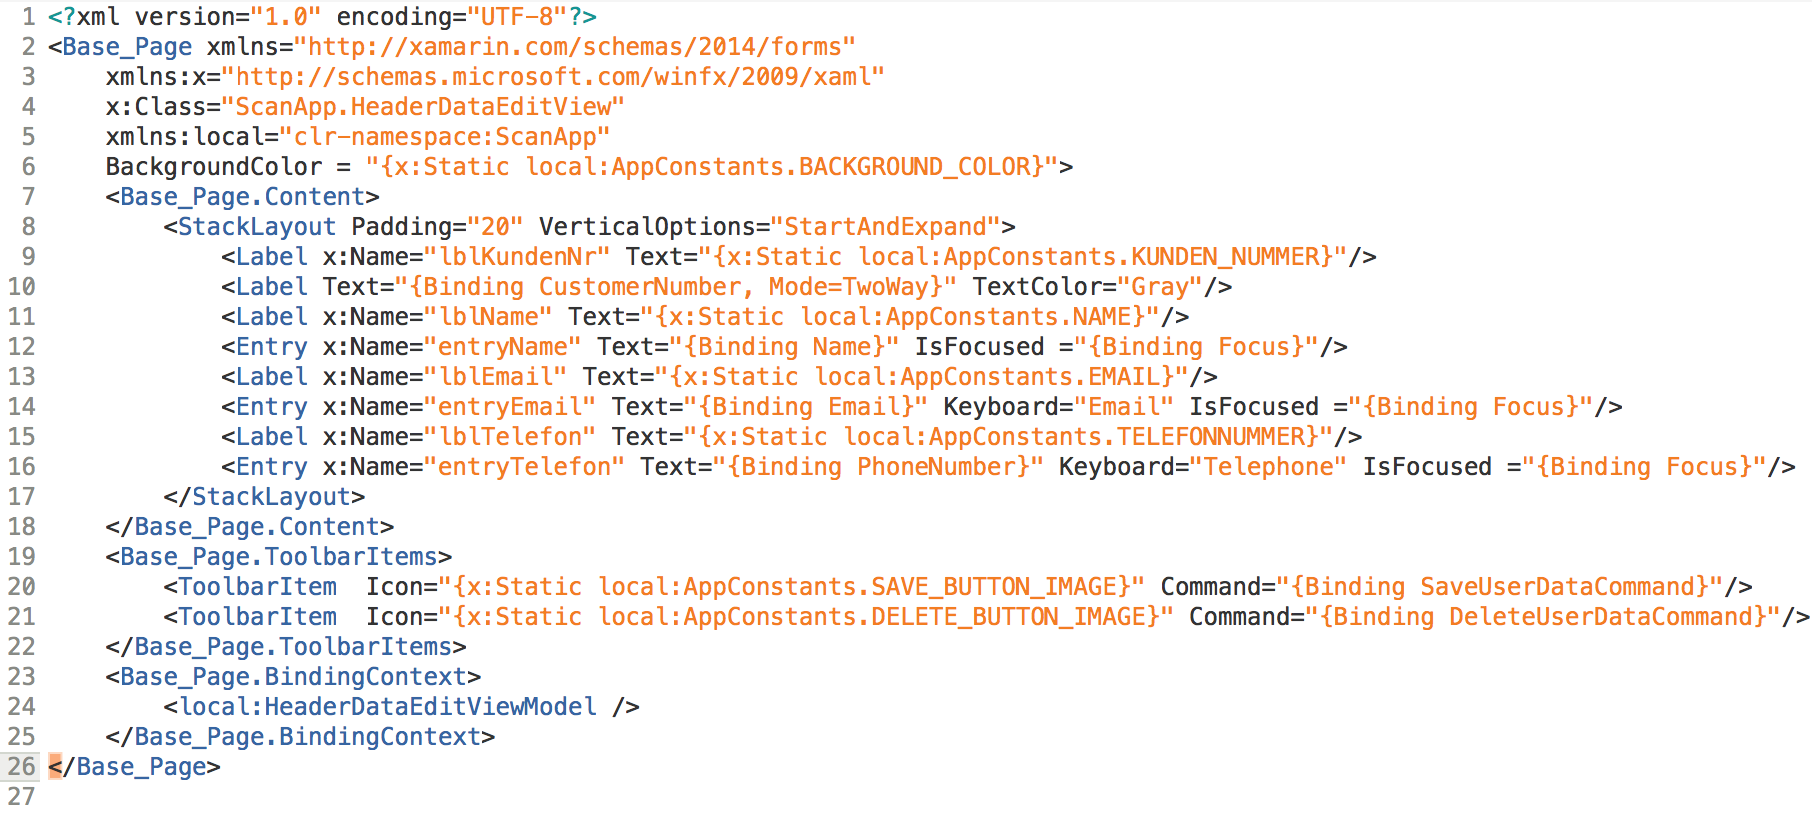
\includegraphics[scale = 0.435]{graphics/Typische_Xaml_Datei.png}
% \caption{Typische Xaml-Datei}
% \label{fig:abb23}
% \end{figure}

% \begin{figure}[!h]
% \centering
% 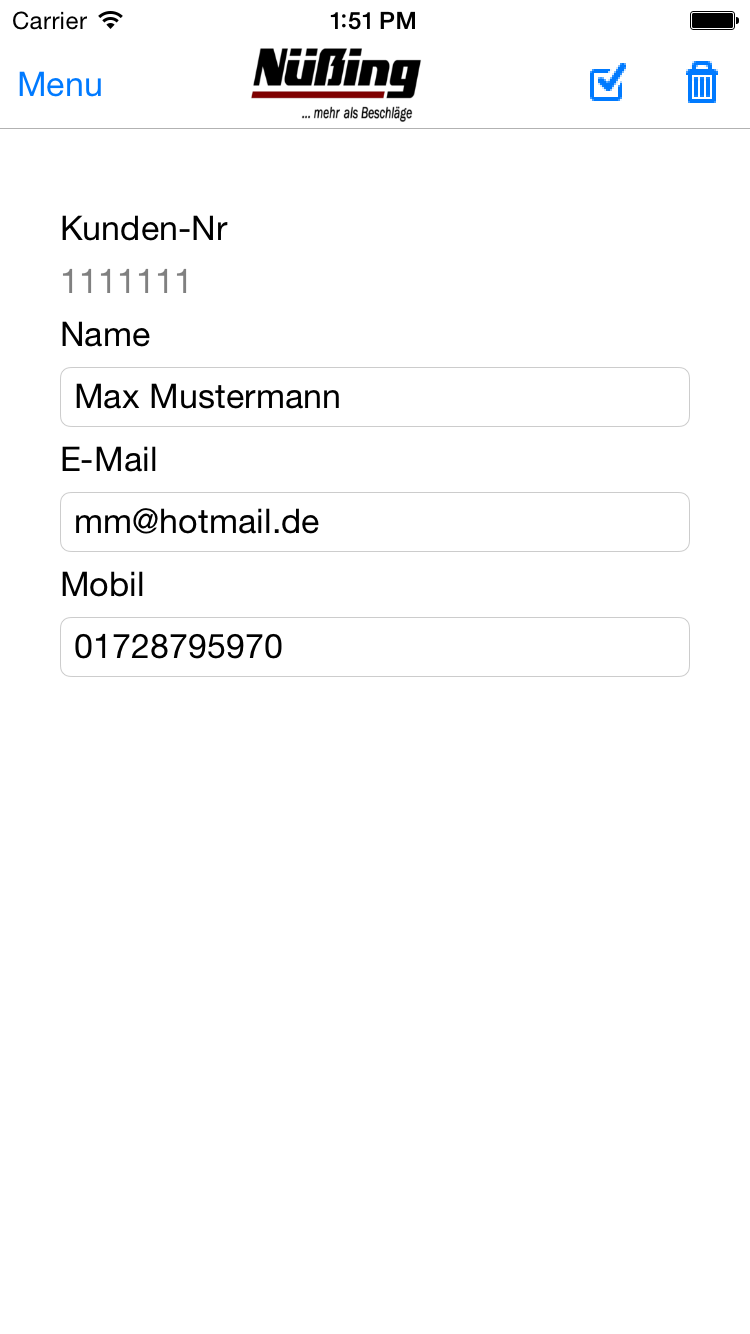
\includegraphics[scale = 0.3]{graphics/appScreenshots/PersoenlicheDaten.png}
% \caption{Screenshot: Seite zum Editieren der pers�nlichen Daten eines Nutzers der ScanApp}
% \label{fig:abb24}
% \end{figure}

% \begin{figure}[!h]
% \centering
% 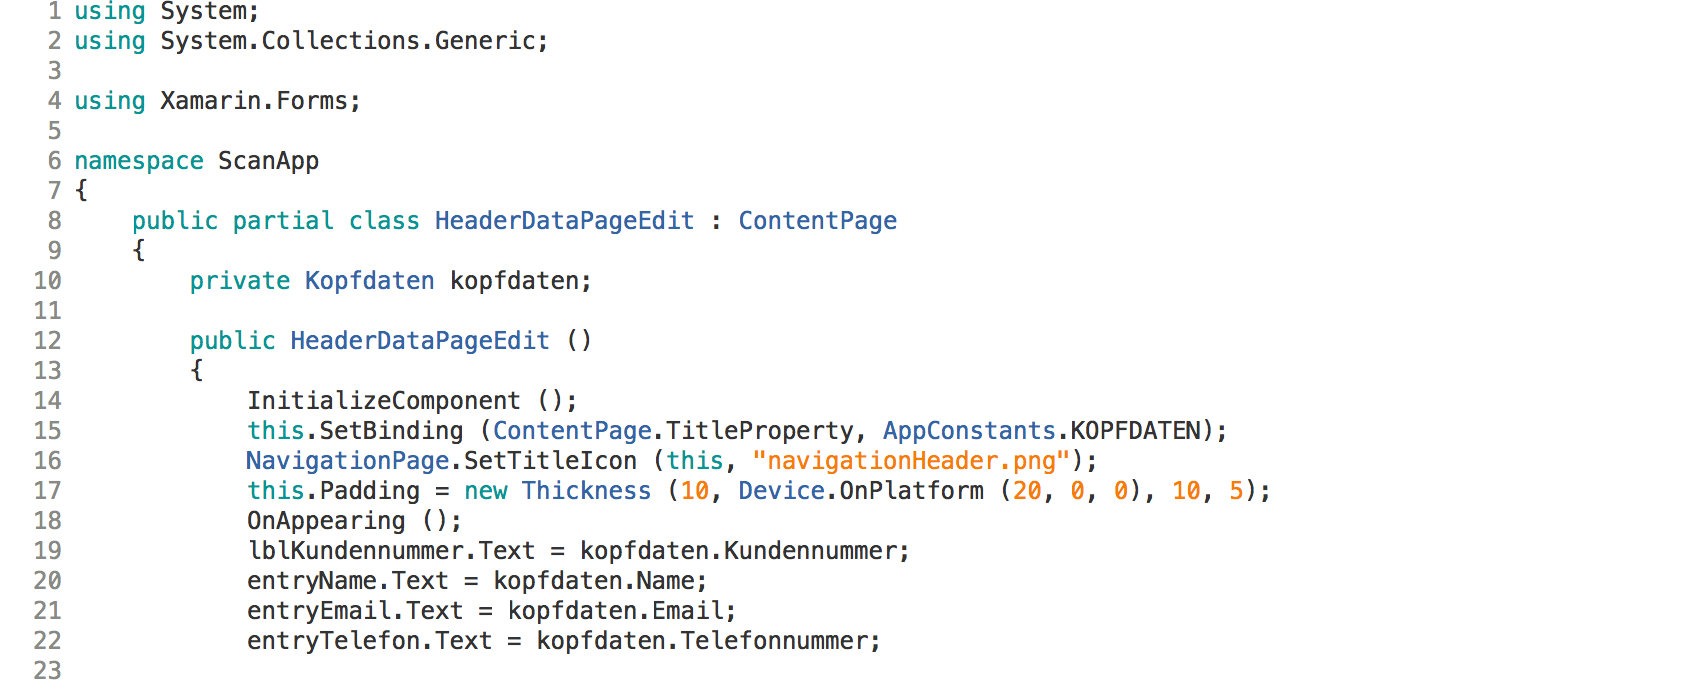
\includegraphics[scale = 0.4]{graphics/HeaderDatenCSDatei.png}
% \caption{Zugrundeliegende (Code-Behind) C\#-Datei}
% \label{fig:abb26}
% \end{figure}


% \begin{figure}[!h]
% \centering
% 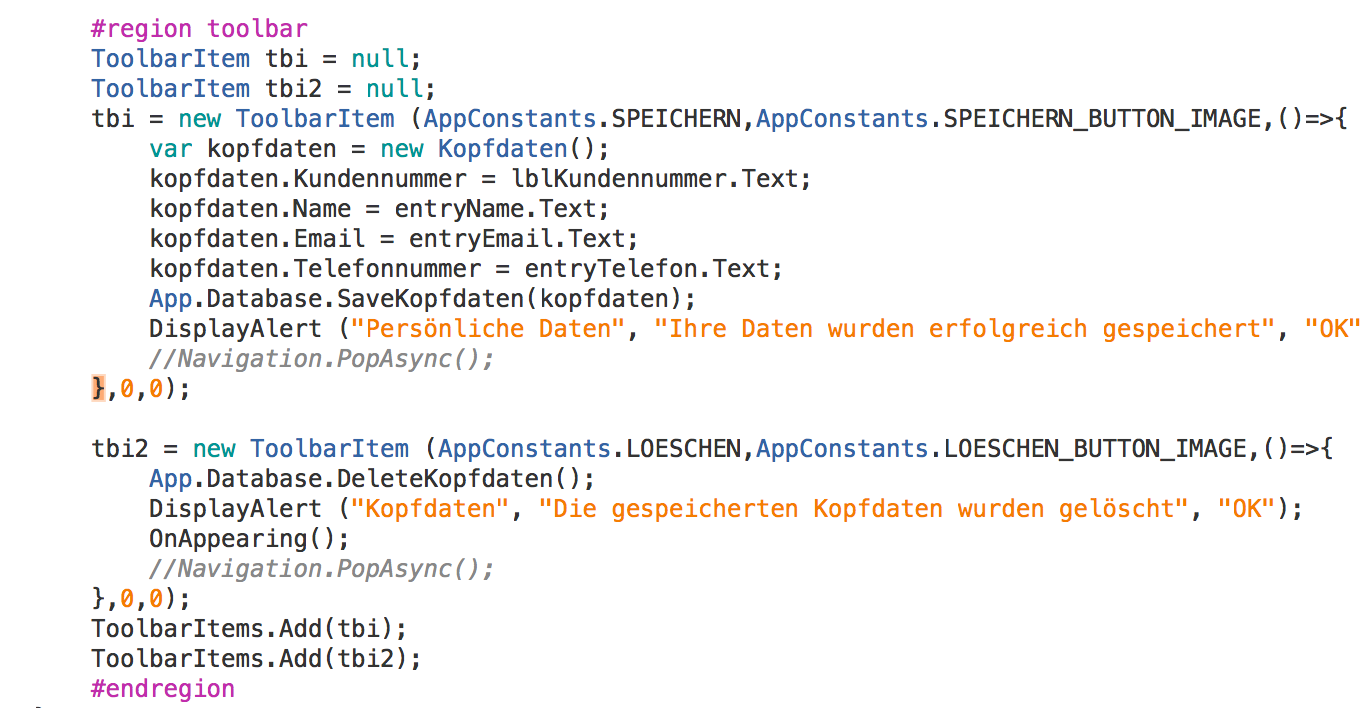
\includegraphics[scale = 0.5]{graphics/HeaderDatenToolbar.png}
% \caption{Zugrundeliegende C\#-Datei}
% \label{fig:abb25}
% \end{figure}

\section{Entwurf der Seiten-Navigation}\label{Navigation} 
Beim erstmaligen Starten der App, wird ein Login-Screen angezeigt (siehe Abb. \ref{fig:abb34}) und der
Benutzer wird aufgefordert sich zu registrieren. Im Falle einer erfolgreichen Registrierung, wird zu der Startansicht
navigiert, n�mlich die Men�f�hrung Ansicht. Nachdem der Benutzer sich einmal registriert hat, wird
die App immer bei dieser Ansicht gestartet.
In \ref{fig:abb39} wird die Navigation zwischen der verschienden Ansichten der App veranschaulicht. 
\\Der User hat folgende Men�positionen zur Auswahl:
\begin{itemize}
  \item Pers�nliche Daten
  \item Bestellungsdaten
  \item Scan
  \item Manuelle Eingabe
  \item Favoriten
  \item Bestellung (Warenkorb)
  \item Scan Historie
  \item Abgeschlossene Bestellungen
  \item Kontakt
\end{itemize}
Je nachdem, welcher Men�punkt ausgew�hlt wurde, wird zu der entsprechenden Ansicht navigiert. Die
Ansichten Scan, Manuelle Eingabe, Favoriten und Scan Historie haben alle gemeinsam, dass beim
Ausw�hlen eines Produkts, bzw. eine Barcodenummer, eine neue Ansicht aufgemacht wird, in der
Informationen �ber das Produkt angezeigt werden. Mit dem "`Back"'-Button kann man dann zur�ck zu der
vorherigen Ansicht navigieren. Bei der Bestellung Ansicht hat man die M�glichkeit, eine
Bestellposition auszuw�hlen, dann wird zu einer Seite navigiert, in der folgende Optionen
angeboten werden:
\begin{itemize}
  \item Bestellmenge �ndern.
  \item Produkt zu den Favoriten hinzuf�gen.
  \item Bestellposition l�schen.
\end{itemize}
Mit dem "`Back"'-Button wird zur�ck zu der Warenkorb-Ansicht navigiert.
In der Ansicht Abgeschlossene Bestellungen kann mit Klick auf eine Bestellung zu einer Ansicht
navigiert werden, in der die einzelnen Bestellungspositionen angezeigt werden. Mit dem
"`Back"'-Button wird zur�cknavigiert.
\begin{figure}[!h]
\centering
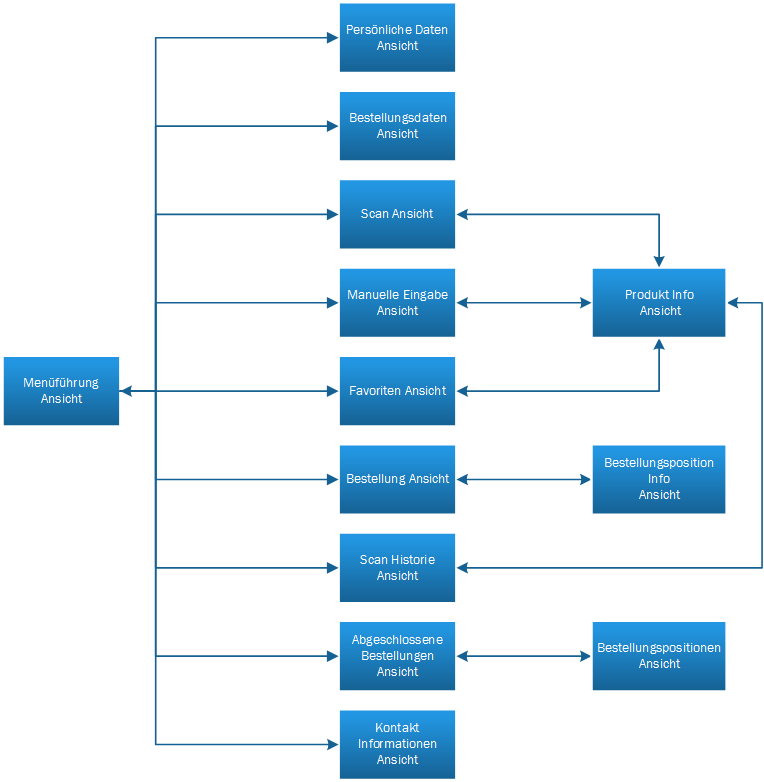
\includegraphics[scale = 0.7]{graphics/ScanApp_Navigation.png}
\caption{Navigation zwischen den Ansichten}
\label{fig:abb39}
\end{figure}
\section{Hardwarenahe Funktionalit�t: Barcodescanner}
Die Struktur der App wurde im "`shared"' Projekt definiert. 
Xamarin.Forms ist eine Art Abstraktionsschicht, man kann es als die Schnittmenge aller
Funktionalit�ten betrachten, die sich im gemeinsamen "`shared"' Projekt implementieren lassen. Die
meisten Funktionalit�ten lassen sich auf diese Weise kapseln und "`cross-plattform"'
implementieren, jedoch gibt es Situationen, in denen ein Feature nicht plattform�bergreifend
umgesetzt werden kann. Typischerweise sind es hardwarenahe Funktionalit�ten, wie bspw. Zugriff auf
spezielle Sensoren des Endger�ts.\\Im vorliegenden Fall ist die Implementierung des Barcodescanners
einer der wenigen Punkten, bei denen ein Eingriff in die plattformspezifischen Projekte notwendig
ist. Sowie zum ScanApp.iOS, als auch zum ScanApp.Droid muss die Xamarin Komponente ZXing.Net.Mobile
hinzugef�gt werden. Diese Komponente greift auf native APIs zu, wie die API zur Steuerung der Kamera des Ger�ts,
um die Scanner-Funktion zu erm�glichen. 
% Da sich diese Funktionalit�t nicht plattform�bergreifend implementieren l�sst, 
% muss das in den zwei
% plattformspezifischen Projekten (ScanApp.iOS und ScanApp.Android) erfolgen. 
In beiden Projekten wird
je eine Klasse Scanner.cs erstellt, in der mithilfe der von der ZXing.Net.Mobile bereitgestellten
API die Funktionalit�t des Scanners implementiert wird. 
\\Der Programmablauf wird im gemeinsamen Projekt gesteuert. Im "`shared"' Projekt wird zu
diesem Zweck ein Interface definiert, das von den Scanner-Klassen der plattformspezifischen Projekte
implementiert wird. Der f�r die Scan-Ansicht zust�ndige ViewModel f�hrt die Methode
ScanClicked() aus, wenn auf den Scan-Button geklickt wird. Der Scanner soll in einem separaten
Thread gestartet werden und erst wenn eine Barcodenummer erkannt wurde, soll es dem Main-Thread
�bergeben werden.

%\subsection{Web Services f�r die Kommunikation mit dem Backend}
% Web Services kommen in den folgenden F�llen zum Einsatz:
% \begin{itemize}
%   \item Bei der einmaligen Registrierung eines Benutzers.
%   \item Beim �berpr�fen eines Barcodes.
%   \item Beim Abschlie�en einer Bestellung.
%   \item Beim Anzeigen des Kundennamen nach der Eingabe einer Kundennummer (Nur im
%   Mitarbeiter-Modus).
% \end{itemize} 
% Im gemeinsamen Projekt wird f�r diesen Zweck eine Klasse mit jeweils eine Methode f�r die oben
% genannten vier F�llen erstellt. Alle Methoden der Klasse benutzen den gleichen Http-Client der
% Komponente \textbf{ModernHttpClient}:\\  
% \textcolor{gray}{\emph{HttpClient client = new HttpClient(new
% ModernHttpClient.NativeMessageHandler())}}.
% \\Wie bei jeder App muss man hier beachten, dass mobile Ger�te nicht selten einen schlechten oder
% gar keinen Empfang haben. Abh�ngig vom Netzwerktyp kann die Geschwindigkeit einer Internetverbindung
% stark variieren. Aus diesem Grund ist es wichtig, dass alle Serveranfragen in einem
% separaten Thread ausgef�hrt werden, so dass der Ablauf der App nicht durch eine schlechte oder
% fehlende Verbindung beeintr�chtigt wird. Au�erdem kann je nach Tarif der mobile Datenvolumen
% begrenzt oder es k�nnen extra Kosten entstehen, wenn eine Bestimmte Grenze von verbrauchten MB pro Monat erreicht
% wird. Aus diesem Grund ist es sinnvoll, dass die App in der Lage ist, den Netzwerktyp zu
% erkennen. D.h. ob die Verbindung �ber WLAN oder �ber das mobile Internet erfolgt. Xamarin.Android
% bietet einen Mechanismus f�r diesen Zweck - durch die Klasse \textbf{NetworkInfo}. Mithilfe dieser Klasse
% kann die App auch erkennen ob Roaming eingeschaltet wurde (\cite{XamNetzwerkStatus}).\\Bei
% Xamarin.iOS gibt es einen �hnlichen Mechanismus.
% \\Der Befehl \textcolor{gray}{\textsl{Reachability.InternetConectionStatus()}} liefert Auskunft
% dar�ber ob eine Internetverbindung �ber WLAN, �ber mobiles Internet erfolgt oder es gar keine
% Verbindung besteht (\cite{XamNetzwerkStatusIOS}). Die Netzwerktyperkennung l�sst sich nicht
% plattform�bergreifend implementieren, das erfolgt in den plattformspezifischen Projekten.
\section{Xamarin Komponenten (Components) und NuGet Packages} \label{nuGetPackages}
Die M�glichkeit, Komponenten und NuGet Packages an ein Projekt anzubinden, ist eine der
gr��ten St�rken von Xamarin.
Da bei Xamarin.Forms Shared Projects keine Komponenten zum gemeinsamen Projekt
hinzugef�gt werden k�nnen, m�ssen die ben�tigten Komponenten zu den
plattformspezifischen Projekten hinzugef�gt werden (siehe Abb. \ref{fig:abb40}).
\subsection{Xamarin Components}
\begin{itemize}
        \item \textbf{ModernHttpClient} - F�r die Kommunikation mit dem Backend wird ein Http-Client
        ben�tigt. Es gibt mehrere �hnliche Komponenten und NuGet Packages. \\F�r die vorliegende
        Arbeit ist die Wahl auf die ModernHttpClient-Komponente gefallen, weil diese          
        vorwiegend sehr positiv in der Xamarin-Community bewertet wird und im Gegensatz zu
        anderen �hnlichen Komponenten auch mit dem Protokol Https funktioniert.
        \item \textbf{ZXing.Net.Mobile} - Die Kernfunktionalit�t der N��ing ScanApp, n�mlich die
        Scan-Funktion wird mithilfe der Xamarin-Komponente ZXing.Net.Mobile gew�hrleistet. Der
        Entwickler braucht sich nicht um native Funktionen, wie die Nutzung der Kamera und das Ein- und Ausschalten des
        Blitzlichtes, zu k�mmern. Diese Funktionalit�t, sowie die Erkennung des Barcodes wird von der
        ZXing-Komponente bereitgestellt. 
\end{itemize}
\subsection{NuGet Packages}
\begin{itemize}
        \item \textbf{Newtonsoft.Json} - F�r die Kommunikation mit dem Backend werden Json-Objekte
        benutzt.
        Damit man zu den in einem Json-Objekt enthaltenen Informationen gelangen kann, muss das Objekt
        zerteilt (geparst) werden. Das NuGet Package Newtonsoft.Json macht das Parsen eines
        Json-Objekts zu einer relativ einfache Aufgabe.
        \item \textbf{Xam.Plugin.DeviceInfo} - Beim ersten Start der Applikation, muss der Kunde sich
        einmalig registrieren. Bei der Registrierung wird auch Information �ber das Ger�t
        mitgesendet. Zu dieser nativen Information gelangt man mithilfe des NuGet Packages,
        Xam.Plugin.DeviceInfo.
\end{itemize}
Es gibt eine gro�e Vielfalt an Xamarin Komponenten und NuGet Packages. Somit kann eine
Xamarin Applikation mit mehreren Features angereichert werden. 
\section{Fazit}
Mit Xamarin.Forms l�sst sich nicht nur die ganze App-Logik im einem Gemeinsamen Projekt
implementieren, sondern auch fast die ganze Benutzungsoberfl�che der App. Daraus resultieren zwei
(oder sogar drei, wenn auch eine Windows Phone als Zielplattform erw�nscht ist) Versionen der
Anwendung, die alle das native "`Look and Feel"' der jeweiligen Plattform haben. Die gemeinsame
Codebasis erleichtert nicht nur den Entwurf, sondern auch das Fixen von Bugs und die Wartung der
App.


\section{Implementierung und Test}
In diesem Abschnitt werden kurz Feststellungen beschrieben, die w�hrend der konktreten Realisierung
der Implementierung der ScanApp aufgefallen sind. Es werden noch typische Testvorg�nge erleutert,
vor allem den Dienst von Xamarin - die Xamarin Test Cloud.
\subsection{Implementierung}
Die Benutzung von Xamarin mit Visual Studio erfordert einen Business-Account. Au�erdem werden zwei
Rechner ben�tigt - ein Mac-Rechner als Build-Server  und ein Windows-PC auf dem Visual Studio l�uft.
Aus diesem Grund fiel die Entwicklungsumgebungswahl f�r die Implementierung der Scan-App die auf
Xamarin Studio. Beim Anlegen einer neuen Solution bietet Xamarin Studio mehrere Solution-Templates
(siehe \ref{fig:abb36}).
\begin{figure}[!h]
\centering
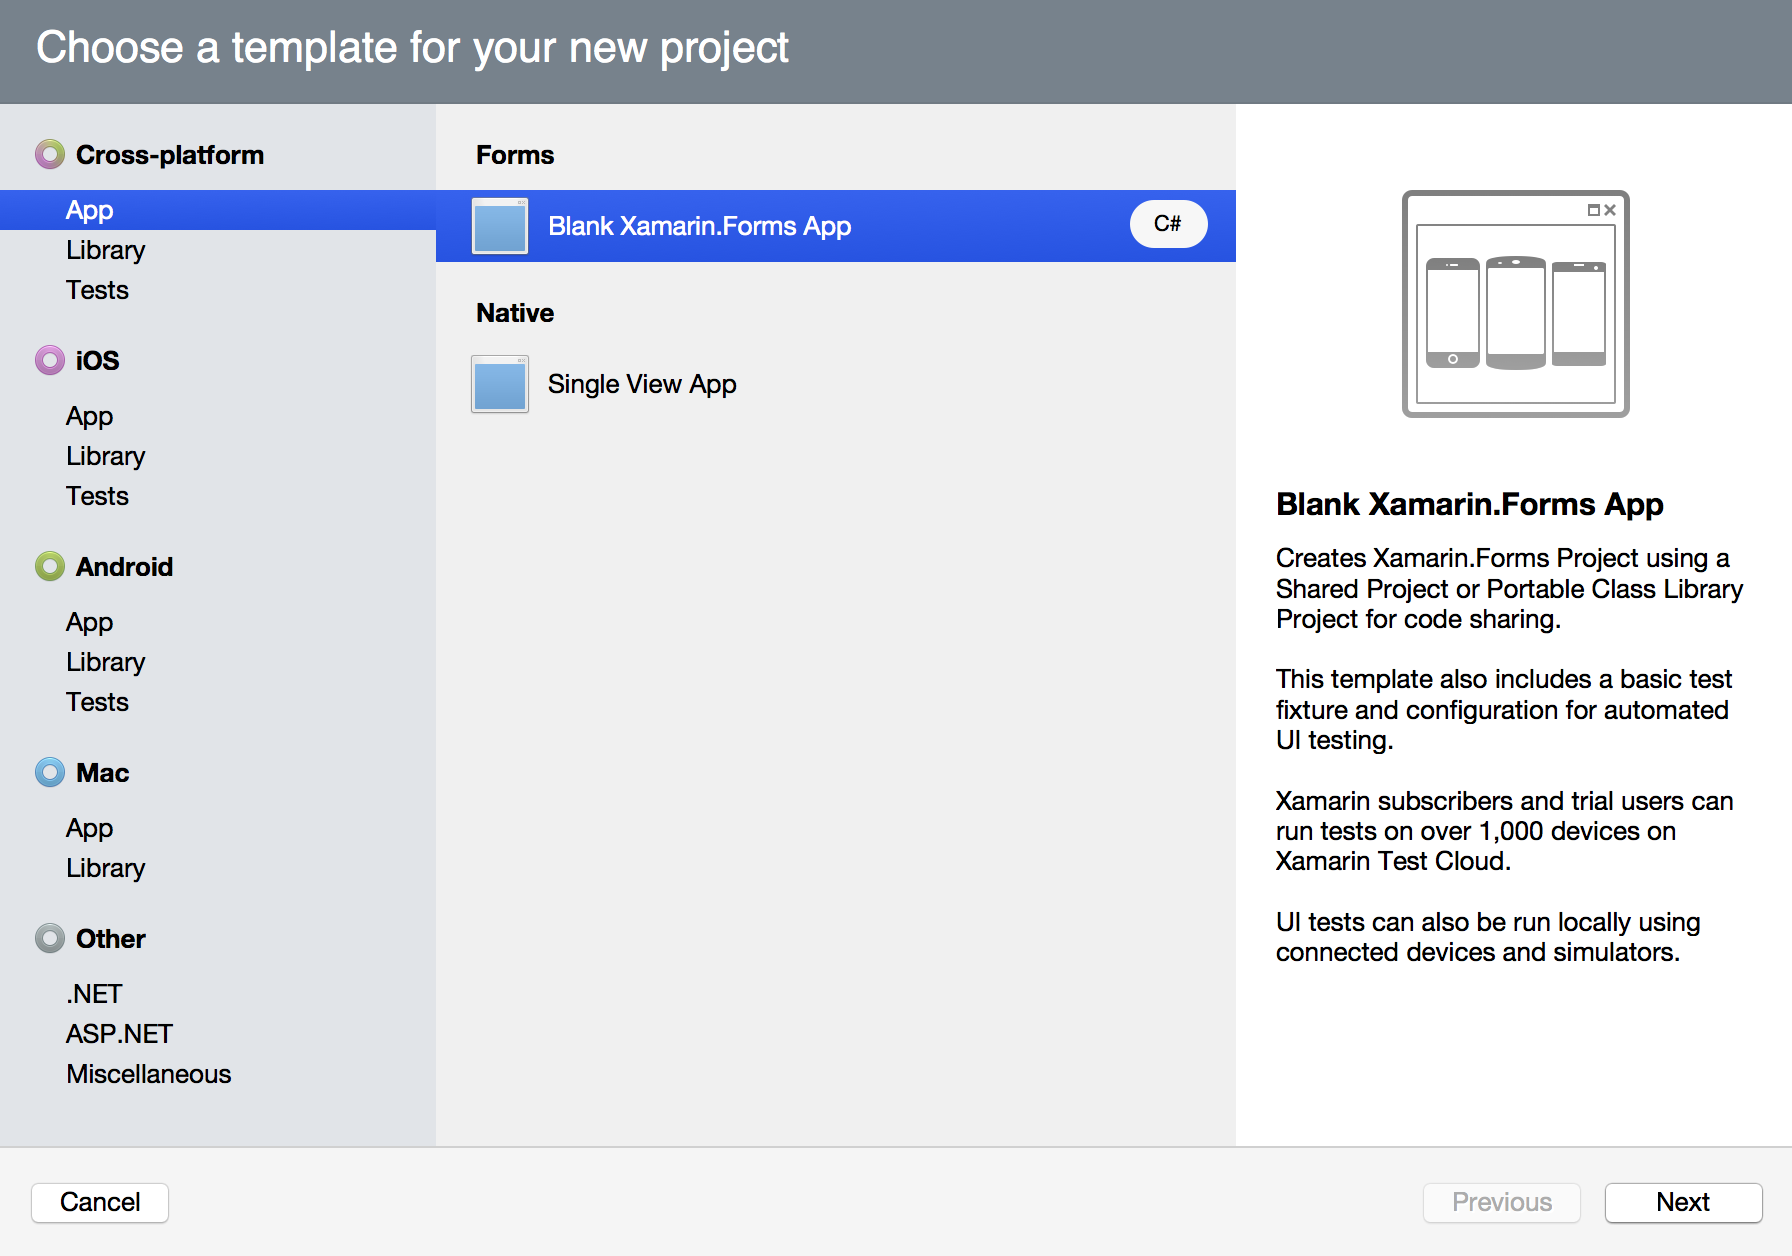
\includegraphics[scale = 0.435]{graphics/XamarinStudioTemplate.png}
\caption{Xamarin Studio Solution Templates}
\label{fig:abb36}
\end{figure}
Beim Erstellen einer neuen Datei bietet Xamarin Studio au�er
Standarddateien C\#-Dateien, wie "`Empty Class"', "`Empty Interface"' usw., noch vorgefertigte
Xamarin.Forms-Dateien, wie "`Forms ContentPage"', "`Forms ContentPage Xaml"', "`Forms Content View"'
oder "`Forms ContentView Xaml"' an. \\Wie bereits im vorherigen Kapitel erl�utert, werden die
Ansichten der App in Xaml implementiert.
Der Aufbau einer Xaml-Datei ist dem Ger�st eines XML-Dokuments sehr �hnlich.
Es gibt ein Wurzelelement und jedes Element kann Attribute besitzen. Dadurch entsteht eine
�bersichtliche Hierarchie der Elemente.
% Durch das Attribut x:Name k�nnte man auf das Element aus der Code-Behind-Datei zugreifen und bspw. den
% Text eines Labels oder die Textfarbe setzen. 
In Abb.\ref{fig:abb23} sieht man eine typische
Xaml-Datei, die eine Ansicht beschreibt und sich im Entwurf beschriebene Ordner View befindet. Diese
Ansicht wird von der benutzerdefinierten Base\_Page abgeleitet, die ihrerseits von der Klasse Xamarin.Forms.Page
abgeleitet wird.
\begin{figure}[!h]
\centering
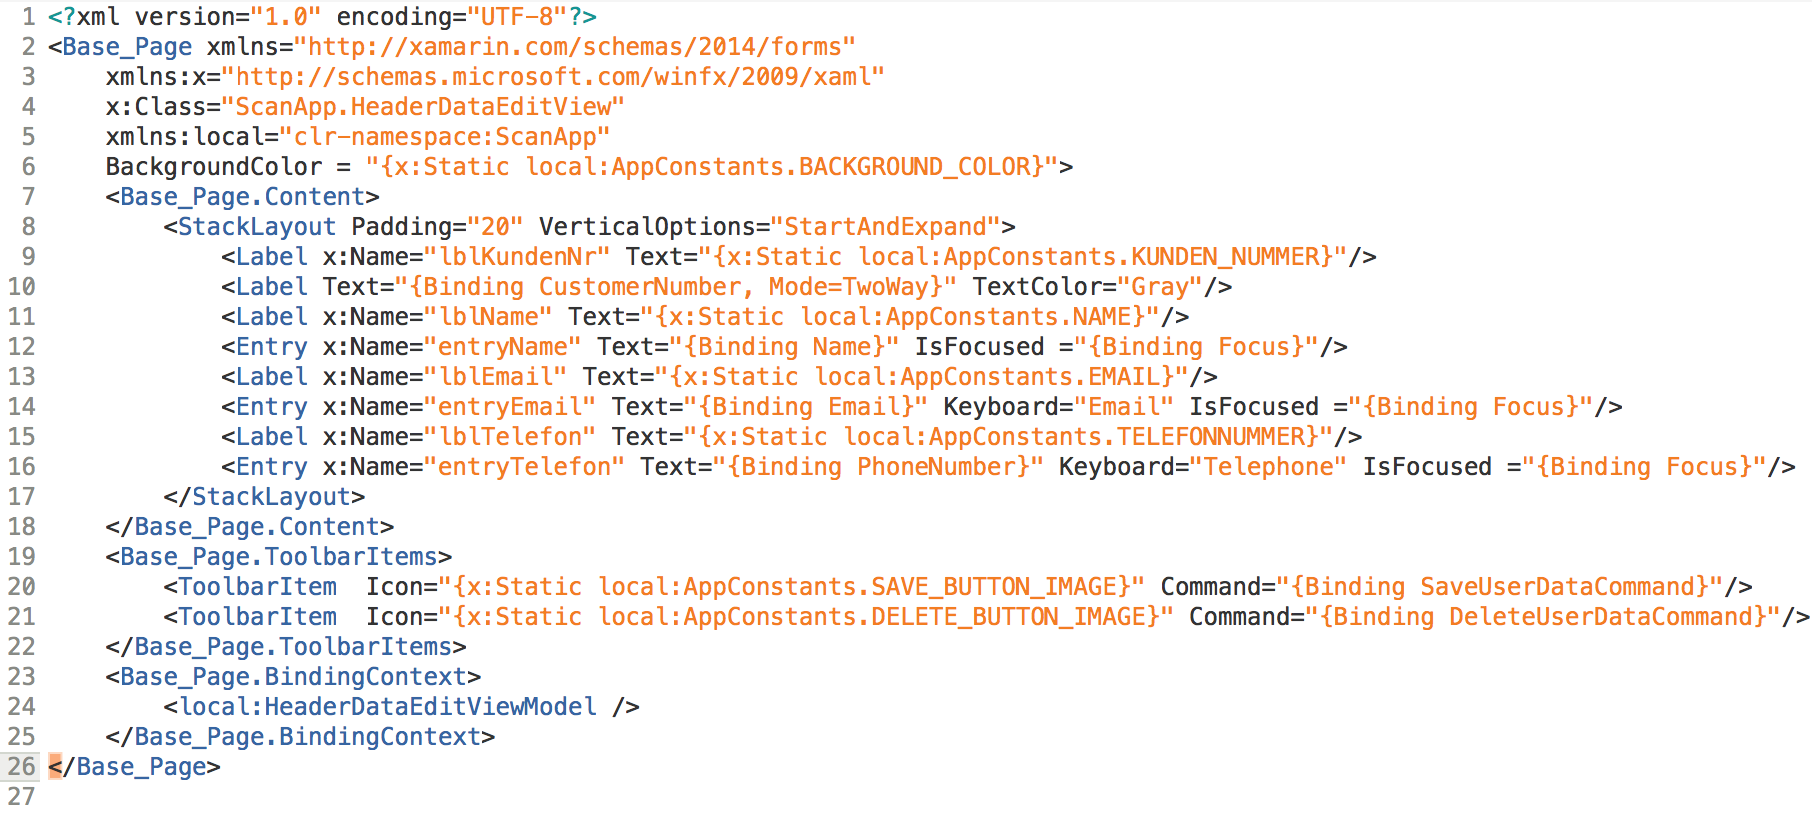
\includegraphics[scale = 0.435]{graphics/Typische_Xaml_Datei.png}
\caption{Typische Xaml-Datei}
\label{fig:abb23}
\end{figure}
\\Eine der wichtigsten Klassenvariablen der Klasse Xamarin.Forms.Page ist das Property
\textit{BindingContext}.
Mithilfe dieser Eigenschaft wird ein Viewmodel (in diesem Fall das HeaderDataEditViewModel) an der Page-Klasse gebunden (Siehe
\ref{fig:abb23}, Zeile 23-25).
\\In Zeile 12 findet eine typische Datenbindung ("`data binding"') statt.
Das Text-Property eines Entry-Textfeldes wird an das Property \textit{Name} gebunden, das im
Viewmodel definiert wird (siehe Abb.\ref{fig:abb33}).
Sobald der Text des Textfelds sich �ndert, wird das Viewmodel dar�ber informiert. Diese Bindung
funktioniert in beiden Richtungen, d.h. �nderungen, die im Viewmodel vorgenommen werden, werden in
der Ansicht angezeigt.\\In Abbildung \ref{fig:abb23}, Zeile 20 ist die Definition eines
Toolbarbuttons zu sehen. Sobald dieser Button gedr�ckt wird, wird ein Command ausgef�hrt, das an
das Property \textit{SaveUserDataCommand} des Viewmodels gebunden ist. D.h. dieses Klick-Event
l�st den Aufruf einer Methode in der Viewmodel-Klasse auf.
\\Durch das Attribut x:Name k�nnte man auf das Element aus der Code-Behind-Datei zugreifen und bspw.
den Text eines Labels oder die Textfarbe setzen.\\Analog lie�en sich auch die anderen Ansichten der
Scan App implementieren. Aus diesem wird nicht n�her ins Detail rangegangen.
% \\Das Ganze veranschaulicht, welche
% Vorteile das MVVM-Architekturmuster mit sich bringt.

\begin{figure}[!h]
\centering
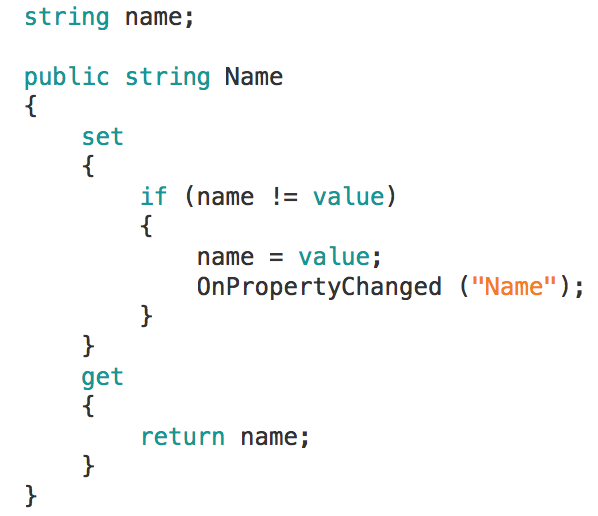
\includegraphics[scale = 0.6]{graphics/Bindable_Property.png}
\caption{Definition von Bindable Property}
\label{fig:abb33}
\end{figure}

\subsection{Test}
Ein wichtiger Schritt im Entwicklungszyklus einer App ist das Testen. Es wird zwischen zwei Arten
von Tests unterschieden, UI- und Unit-Tests. 
W�hrend Unit-Tests die App-Logik testen, wird bei UI-Tests sichergestellt, dass die App so aussieht
und sich so verh�lt, wie man es erwartet, also es wird das Optische getestet.\\Ein typischer Weg,
eine App zu testen ist die Anwendung zu starten und zu benutzen.
Im besten Fall tut die App genau das was sie tun soll - funktioniert korrekt und st�rzt nicht ab. Erfahrungsgem�� ist das so
gut wie nie der Fall. Diese Art von Testen, indem man die App auf einem realen Ger�t nutzt, wird als UI
Acceptance Testing bezeichnet.
Die zur Verf�gung gestellten Simulatoren erleichtern wesentlich den Testprozess, allerdings um
sicher zu gehen, dass eine App wirklich fehlerfrei funktioniert, kommt man an Tests auf reale Ger�te nicht
herum. Da es vor allem bei Android eine gro�e Vielfalt an Ger�ten gibt, kann das sehr m�hsam sein.
Softwarehersteller m�ssen nicht selten Apps auf dutzende sogar hunderte Ger�te installieren und
testen.\\Die meisten Developer verzichten auf systematisches Testen, weil die verf�gbaren Tools und
Dienste zu kompliziert und schwer zu benutzen sind und nur auf einem Ger�t bzw. Simulator ausgef�hrt
werden k�nnen. \\Abhilfe kann man sich bei einem Dienst von Xamarin, genannt Xamarin Test Cloud,
schaffen.\\Alle Xamarin-Plattform-Abonnements beinhalten 60 Xamarin Test Cloud Ger�te-Minuten pro Monat. D.h. jeder Entwickler, der einen Xamarin Account hat,
kann die Dienste der Xamarin Test Cloud in Anspruch nehmen.
Xamarin verf�gt �ber 1600 reale iOS- und Android-Smartphones und Tabletts. An dieser Stelle muss
klargestellt werden, dass es allerdings nur iOS- und Android-Ger�te sind, also die Test Cloud von
Xamarin unterst�tzt noch nicht Windows Phone.
Mit der Test Cloud kann man leicht visuelle Inkonsistenzen feststellen, indem man die Ergebnisse eines UI-Tests auf
dutzende Ger�ten vergleicht. Der Entwickler hat die M�glichkeit Screenshots an beliebigen Stellen
des Tests zu machen.
Dar�ber hinaus bietet der Service auch Videoaufnahme von Tests.
Eine Ger�te-Minute wird konsumiert, wenn der Test auf einem Ger�t ausgef�hrt wird, wobei es keine
Rolle spielt ob die Tests parallel auf mehrere Ger�te oder nacheinander ausgef�hrt werden.\\Beim
Anlegen der Xamarin.Forms Solution, wurde au�er des plattform�bergreifenden Projekt und der
plattformspezifischen Projekte noch ein weiteres Projekt angelegt - das
ScanApp.UITests Projekt.
In diesem vorgefertigten Projekt befinden sich die Klassen: AppInitializer.cs und Tests.cs.\\In
AppInitializer werden Konfigurierugen vorgenommen, wie Angabe des Pfads der Android APK Datei und
der iOS IPA Datei. In der Klasse Tests.cs werden die Tests implementiert. Eine sogenannte
TestFixture umfasst mehrere Test-Methoden. Auf diese Klasse wird sp�ter n�her eingegangen.
\\Xamarin.UITest
basiert auf Calabash, eins der ber�hmtesten Frameworks f�r automatisiertes Testen von mobilen Apps.
Solche Tests setzen auf den Xamarin Test Cloud Agent auf, einen speziellen HTTP-Server, der mit der
zu testenden mobilen Applikation kommuniziert.
Der Xamarin Test Cloud Agent muss eingebettet in die iOS Applikationen sein, wenn die App
kompiliert wird. Bei Android Applikationen ist der TestCloud Agent eine separate Anwendung, die
neben der zu testende App installiert wird. Die Tests interagieren mit der UI als w�rde ein Benutzer
in Wirklichkeit Text ein ein Entry-Feld eintippen, irgendeine Geste durchf�hren, oder auf einen Button klicken usw.
% Nachdem die Tests geschrieben worden sind, kann man die lokal ausf�hren und wenn die Tests
% erfolgreich abgeschlossen wurden, kann man die auch in der Cloud ausf�hren lassen.
Solche Tests k�nnen lokal ausgef�hrt werden und erleichtern die Entwicklung einer App. Die
eigentliche St�rke von Xamarin.UITest ist, allerdings, die M�glichkeit, diese lokale Tests in die
Xamarin Test Cloud hochzuladen. In der Cloud steht eine Vielzahl von realen Ger�ten (alle ohne
Jailbreak) zur Verf�gung. Xamarin Test Cloud generiert bei jedem Schritt eines Testfalls Screenshots von der App.
Somit kann der Developer einen Vergleich zwischen den Darstellungen seiner App auf den verschiedenen
Ger�ten ziehen. Screenshots k�nnen allerdings nicht alle Benutzereindr�cke abbilden. F�r diesen
Zweck ist auch ein Screen Recording m�glich.

Typischerweise wird jeder UITest als eine Methode definiert. Die Klasse, die den Test enth�lt, wird als Test Fixture bezeichnet. Eine Text Fixture enth�lt entweder einen Test oder eine logische Gruppe von Tests. 
Sie ist f�r Einstellungen und Bereingungen, die nach den Tests durchgef�hrt werden sollen zust�ndig.
Jeder Test sollte dem "`arrange-act-assert"' Muster folgen (siehe Abb. \ref{fig:abb37}):
\begin{itemize}
  \item Vereinbarungen treffen (arranging) - Vorbereitungen f�r den Test. D.h. hier werden
  Bedingunen eingestellt und Initialisierungen durchgef�hrt, so dass der Test gestartet werden kann.
  \item Handeln (acting) - Interaktionen mit der App, wie Eintippen von Text, Klicken auf Buttons
  usw.
  \item Behauptungen �berpr�fen (asserting) - hier werden die Ergebnisse der Interaktionen auf
  Korrektheit �berpr�ft
\end{itemize}
\begin{figure}[!h]
\centering
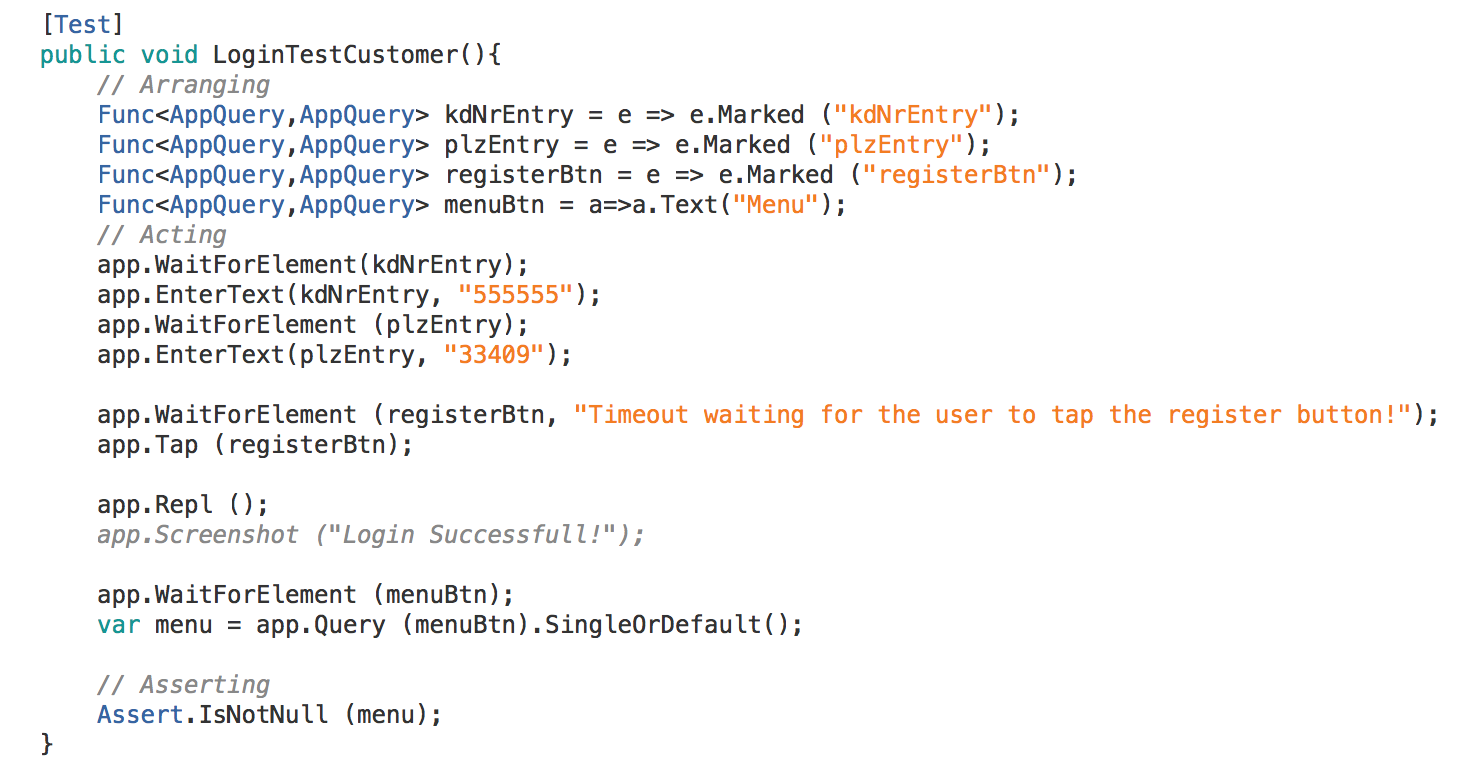
\includegraphics[scale = 0.565]{graphics/XamarinUITest.png}
\caption{Xamarin.UITest}
\label{fig:abb37}
\end{figure}
Xamarin.UITests setzen auf Queries auf, um Views auf dem Screen zu lokalisieren. Diese Queries
benutzen Attributen der Views, wie Identifier, und nicht die physiche Position der Views auf dem
Screen. Dies ist eine sehr m�chtige Technik, die es Xamarin.UITest erlaubt mit den Objekten zu
interagieren, unabh�ngig von Bildschirmgr��e, Orientierung oder Layout. Xamarin.UITest bietet ein
REPL (read eval print loop) an, das sehr hilfreich beim Erstellen einer solchen Query sein kann.
REPL erlaubt Entwicklern, mit der Anwendung zu interagieren, w�hrend es l�uft.
Um einen Xamarin.UITest zum laufen zu bringen, muss das NuGet Package Xamarin Test Cloud Agent zum
iOS-Projekt hinzugef�gt werden. Bei Xamarin.Android ist das nicht erforderlich. Allerdings braucht
man bei Android eine APK-Datei. D.h. JDK und Android SDK m�ssen installiert sein. In den meisten
F�llen werden die aber mitinstalliert bei der Installation von Xamarin.Android (\cite{XamUITest}).

\begin{figure}[!h]
\centering
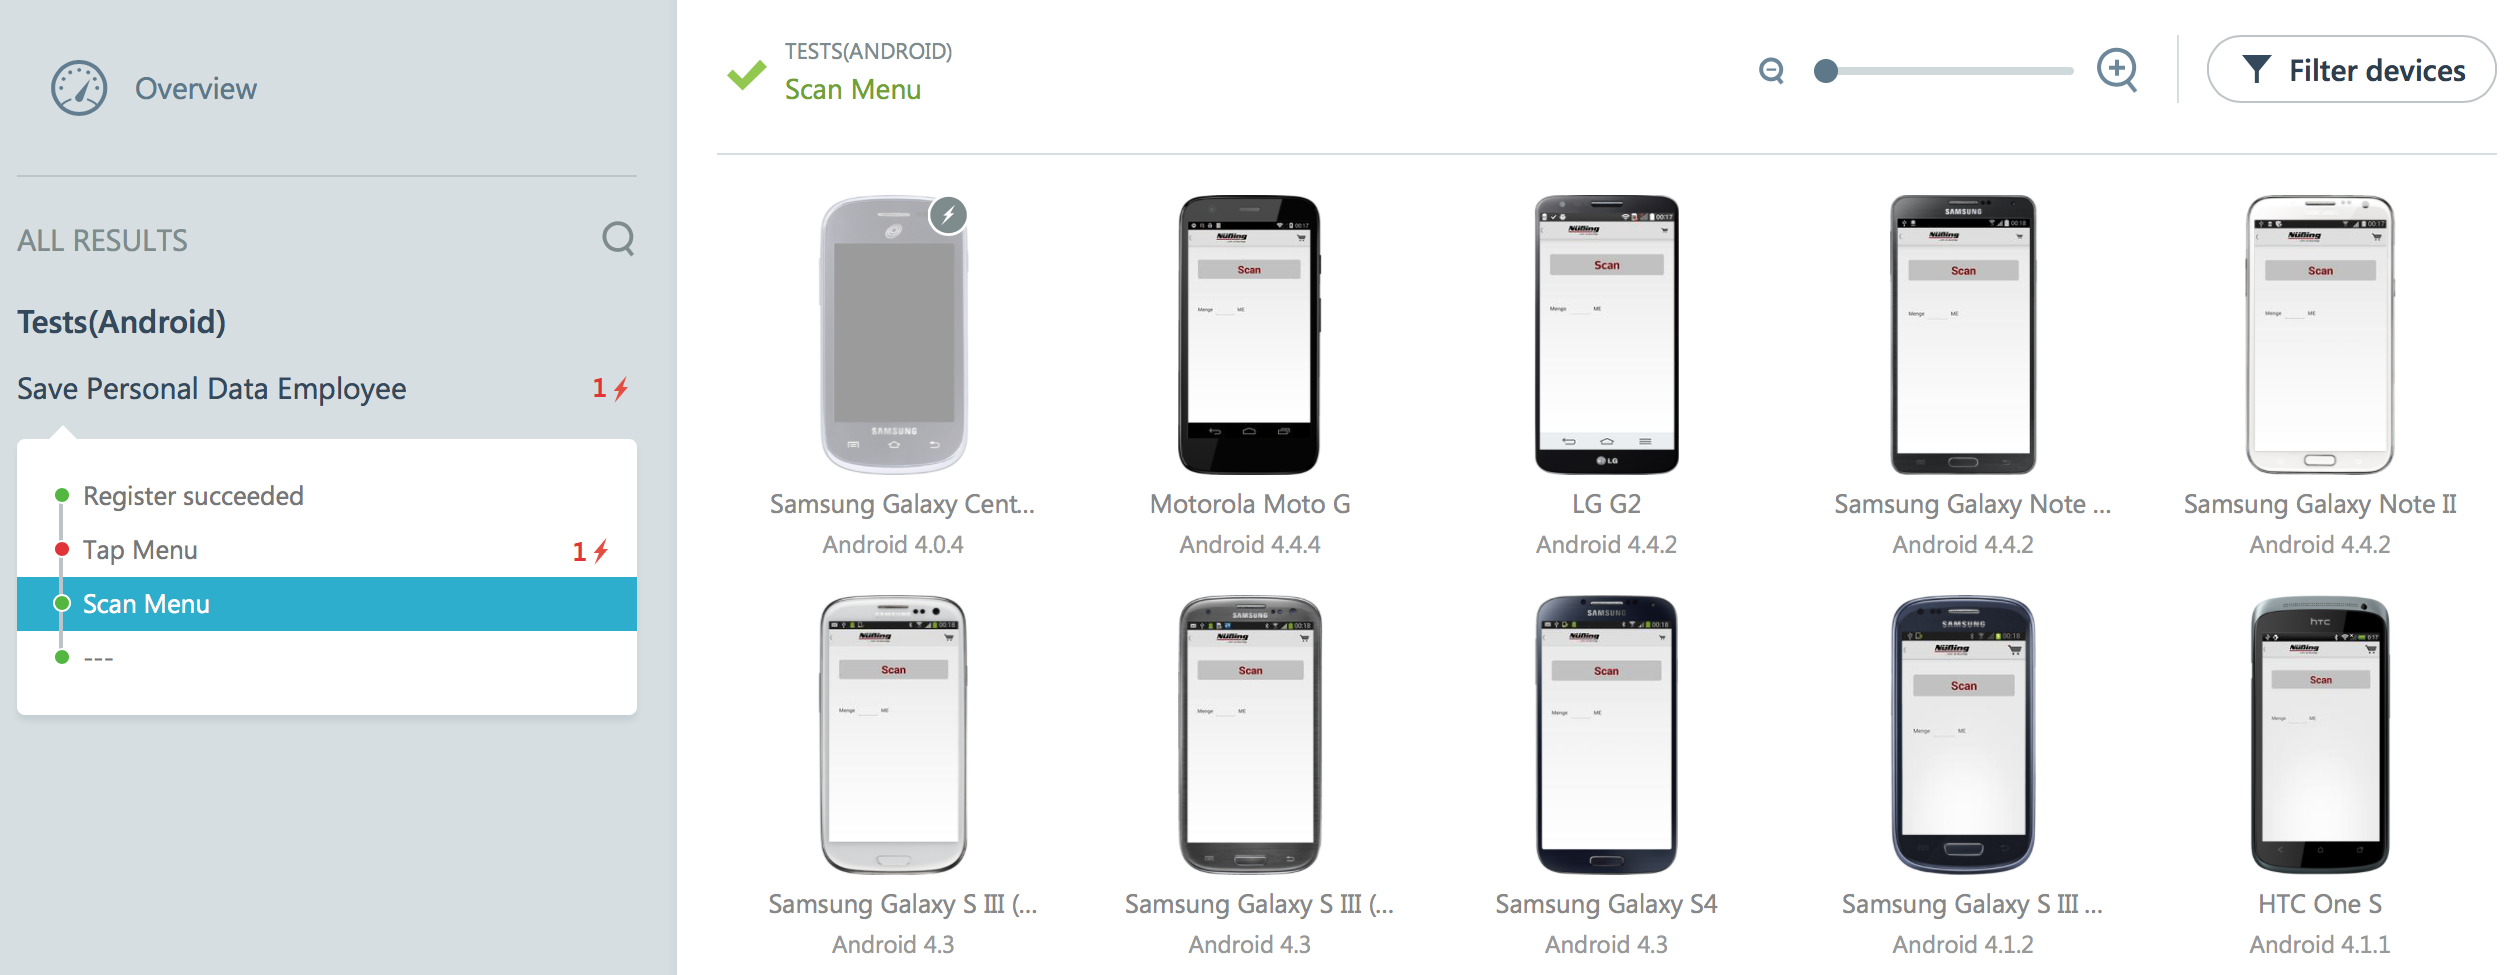
\includegraphics[scale = 0.15]{graphics/XamarinTestCloud.png}
\caption{Xamarin Test Cloud}
\label{fig:abb35}
\end{figure}


\chapter{Evaluierung inkl. Bewertungskriterien}
Die beste Art und Weise ein Cross-Plattform-Entwicklungsframework zu bewerten ist, die Qualit�t
eines Software-Produkts, das mit dieser Technologie entwickelt wurde zu bewerten. Im vorliegenden
Fall ist es die Scan-App.\\\textbf{ISO/IEC 9126} definiert Software-Qualit�t als:\\ \emph{
Gesamtheit von Merkmalen und Merkmalswerten eines Software-Produkts, die sich auf dessen Eignung
beziehen, festgelegte oder vorausgesetzte Erfordernisse zu erf�llen}.
\\Um die Qualit�t eines
Software-Produkts bewerten zu k�nnen, werden m�glichst objektive pr�fbare Kriterien ben�tigt.


\section{Bewertungskriterien nach ISO-Norm 9126}
Im Folgenden werden Qualit�tsmerkmale nach \textbf{ISO-Norm 9126} vorgestellt. Anhand dieser
Kriterien wird die App bewertet. In Abb.\ref{fig:abb38} werden die ISO-Norm 9126
Softwarequalit�tsmerkmale abgebildet.
\begin{figure}[!h]
\centering
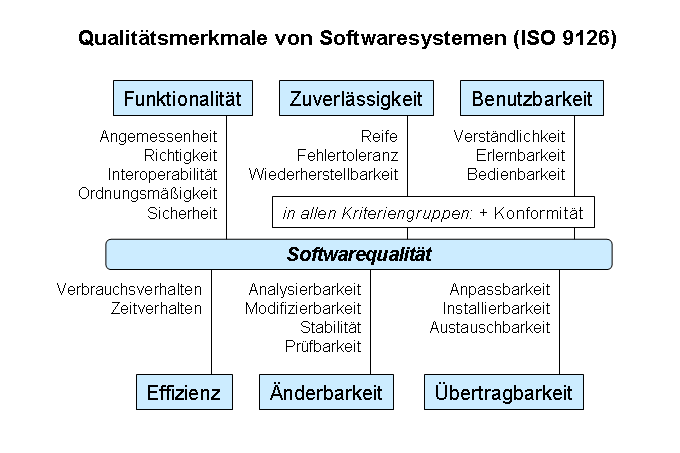
\includegraphics[scale = 0.805]{graphics/ISO_9126_Grafik.png}
\caption{Softwarequalit�t nach ISO-Norm 9126 (Quelle:\cite{SWQGrafikWiki})}
\label{fig:abb38}
\end{figure}
\subsection{Funktionalit�t}
\subsubsection{Interoperabilit�t}
Die Kommunikation zwischen der App und dem Server wurde auf verschiedene Szenarien getestet. Es
wurde sichergestellt, dass die App nicht abst�rzt, wenn der Server nicht erreichbar ist.
\subsubsection{Sicherheit}
F�r eine sichere Kommunikation mit dem Backend, generiert die App mithilfe des
Verschl�sselungsalgorithmus SHA-256 einen Adresszusatz f�r die Web Services URI. Dar�ber hinaus wird
das Https Protokol benutzt.
\subsubsection{Richtigkeit}
%Sind alle geforderten Funktionen implementiert worden?
Im vorangegangenen Kapitel wurden Anforderungen an die App spezifiziert und anschlie�end
wurde die Anwendung nach diesen Kriterien getestet. D.h. alle geforderten Funktionen sind in beiden
Versionen der App (iOS und Android) implementiert worden und somit ist dieses Kriterium erf�llt.
\subsection{Zuverl�ssigkeit}
Dank Xamarin Test Cloud wurde die Zuverl�ssigkeit der Scan-App getestet. Aufgrund der gro�en
Vielfalt an Android-Smartphones wurde besonders bei der Android Version darauf geachtet, dass die
App auf m�glichst vielen Ger�ten getestet wird. Es wurden unterschiedliche Szenarien durchgespielt,
die eventuell zum Absturz der App f�hren k�nnten. Es wurde das Verhalten der Anwendung beobachtet,
wenn bspw. die Internetverbindung w�hrend einer Anfrage an den Server unterbrochen wird, oder bei
einem unerwarteten Ausschalten des Telefons, durften keine keine zuvor
gespeicherten Daten verloren gehen. Da die iOS- und die Android-Version der App die Tests
erfolgreich abgeschlossen haben, l�sst sich schlie�en, dass das Kriterium Zuverl�ssigkeit erf�llt
ist.
\subsection{Benutzbarkeit}
F�r die Scan-App wurde eine intuitive Benutzbarkeit angestrebt. F�r die Men�punkten wurden
aussagekr�ftigen Namen ausgew�hlt, so dass f�r die Benutzung der Anwendung keine Schulung
vorausgesetzt wird.
\subsection{Effizienz}
Die mobilen Ger�te werden immer leistungsf�higer, allerdings aufgrund der gro�en hochaufl�senden
Displays halten die Akkus nicht besonders lange. Aus diesem Grund werden Anwendungen, die zu viel
Akku im Hintergrund verbrauchen, oft von den Benutzern abgelehnt, auch wenn die App sonst prima
funktioniert.\\Xamarin.Forms bietet die M�glichkeit die Methoden \textit{onStart(), onSleep() und
onResume()} zu �berschreiben und somit l�sst sich das Verhalten der App steuern, wenn die Anwendung
im Hintergrund ger�t.\\Bei der Entwicklung der App wurde explizit darauf geachtet, dass die
Kommunikation mit dem Server in separaten Threads ausgef�hrt wird, so dass die App nicht "`h�ngen
bleibt"', wenn die Internetverbindung langsam ist oder gar nicht da ist.
\subsection{�nderbarkeit}
Die "`Hamburger"'-Men�f�hrung der App erlaubt eine Erweiterung oder �nderung des Men�s um beliebig
viele neue Men�positionen.
Aufgrund der gemeinsamen Logik lassen sich �nderungen und Fehlerkorrekturen der App mit m�glichst
wenig Aufwand im gemeinsamen Projekt vornehmen. Kriterium erf�llt.
\subsection{�bertragbarkeit}
Durch die Distribution der ScanApp in die entsprechenden App-Stores (Apples App Store und
Androids Google Play Store) kann die Scan-App auf die �bliche Art und Weise
verbreitet werden. Kriterium erf�llt.
\section{Weitere Bewertungskriterien}
Ausser der ISO Standards sind im vorliegenden Fall auch folgende Bewertungskriterien sinnvoll:
\begin{itemize}
  \item Es soll eine plattform�bergreifende Programmiersprache benutzt werden.
  \item Gute Unterst�tzung durch IDE.
  \item Das Framework soll Zugriff auf native Elemente, wie bspw. die Kamera eines Smartphones
  erm�glichen.
  \item Klare Trennung zwischen UI und Business Logik.
  \item Code-Sharing: Der Code-Sharing Anteil soll mehr als 50\% des Gesamtcodes sein.
  \item Gesch�ftslogik soll einmal in dem gemeinsamen Projekt implementiert werden und nicht in den
  plattformspezifischen Projekten.
  \item UI-Konzept - die von der Entwicklungsplattform bereitgestellten UI-Tools, sollen die
  Funktionalit�t einer nativ entwickelten App gew�hrleisten k�nnen.
  \item Persistieren der Daten (Datenbankanbindung) soll unterst�tzt werden.
  \item Es sollen m�glichst wenig Bugs w�hrend des Entwicklungsprozesses entstehen und deren
  Behebung soll nicht mit viel Aufwand verbunden sein.
  \item Die mit Xamarin entwickelte mobile Anwendung soll keine funktionale Unterschiede zu einer
  nativen Applikation aufweisen.
  \item Soll nicht deutlich langsamer als die Referenz Applikation sein.
  \item Die Distribution einer mit Xamarin entwickelten Anwendung in die entsprechenden App-Stores
  soll mit einem �hnlich gro�en Aufwand verbunden sein, wie die Distribution einer nativen App.
\end{itemize}
\section{Feststellungen}
\subsection{Positive Feststellungen}
Es muss erw�hnt werden, dass das Team von Xamarin sich gro�e M�he f�r die Weiterentwicklung des
Frameworks gibt.
Bspw.
wenn Apple neue APIs vorstellt, k�nnen die innerhalb weniger Stunden mit Xamarin verwendet werden. 
Es finden regelm��ige Updates und Bugfixes statt.
\subsection{Negative Feststellungen}
\subsubsection{MVVM}
Aufgrund der nicht sehr ausf�hrlichen Informationen auf der offiziellen Seite von Xamarin ist es
keine einfache Aufgabe, sich an dem MVVM-Architekturmuster zu halten. 
Es ist zu beobachten, dass in vielen der Beispielen aus dem Netz, die ganze Funktionalit�t einer
Ansicht(Xaml-Datei) in der dazugeh�renden Code-Behind-Datei untergebracht wird, was die Idee
des MVVMs und die lose Kopplung zwischen View und Viewmodel zunichte macht. 
\\F�r einen Entwickler ohne Erfahrung mit dem MVVM-Entwurfsmuster kann das sehr irref�hrend sein.
In den Beispielen, in denen das MVVM-Pattern sauber angewendet wird, werden oft lediglich einfache
Szenarien beschrieben, ohne komplizierte Interaktionen, wie z.B. Navigation zwischen den
Ansichten, so dass es f�r einen Anf�nger eine richtige Strukturierung einer App zu einer
r�tselhaften Aufgabe werden k�nnte. Es wird den Eindruck hinterlassen, dass Xamarin noch nicht ganz
ausgereift f�r MVVM ist.
\subsubsection{HTTPS}
Wie bereits erw�hnt wird das Protokol https benutzt, um eine sichere Kommunikation mit dem
Backend, in einer unsicheren Umgebung, zu gew�hrleisten. F�r die Nutzung von Web Services wird in
der Xamarin Comunity das NuGet Package \textit{Microsoft.Net.Http} empfohlen. Der in diesem Package
enthaltene Http-Client weist allerdings Schw�chen auf, wenn die Kommunikation wie im vorliegenden
Fall nicht �ber http sondern �ber https erfolgen soll. Diese Schw�chen sind kaum
dokumentiert und es kann lange dauern bis der Entwickler auf die Fehlerquelle kommt.
\subsubsection{Die Gr��e der IPA-Datei}
Die Datei ist gr��er als die IPA-Datei einer nativ entwickelten iOS-App.
\section{Grenzen der Cross-Plattform-Entwicklung}
Xamarin entwickelt sich mit raschem Tempo. Xamarin.iOS und Xamarin.Android bieten
.NET Entwicklern, die M�glichkeit Apps f�r iOS und Android zu entwickeln, die kaum von den
nativ entwickelten iOS- und Android-Apps zu unterscheiden sind. \\Interessant f�r die vorliegende
Arbeit ist der Ansatz von Xamarin.Forms. Wie im Kapitel 4.4.1.
bereits erl�utert, haben Entwickler f�nf verschiedenen Arten von Ansichten zur Auswahl, um  eine
Seite (Page) mit Xamarin.Forms zu erstellen. F�r die Implementierung der ScanApp werden lediglich
ContentPages, NavigationPages und eine MasterDetailPage f�r die Men�steuerung benutzt. \\Sollte es speziellere Anforderungen an der
Benutzeroberfl�che geben, m�ssen Entwickler sogenannte "`custom renderer"' benutzen, um auf native
plattformspezifische SDK-Features zugreifen zu k�nnen. Allerdings befinden sich die Xamarin
Renderer-APIs noch in einer Bearbeitungsphase (\cite{XamarinCustomRenderer}) und allem Anschein nach wird es noch
einige Zeit dauern bis Xamarin die M�chtigkeit der herk�mmlichen nativen App Entwicklung erreichen
kann.\\Es wurden oft die Vorteile der m�chtigen .NET Plattform erw�hnt. Allerdings muss beachtet
werden, dass Xamarin nicht alle diese Vorteile nutzen kann, weil Xamarin nicht direkt auf .NET
basiert, sondern auf das Open-Source-Projekt Mono. D.h. Xamarin-Developer haben nur
eine Teilmenge der Funktionalit�ten von .NET zur Verf�gung.



\chapter{Zusammenfassung und Ausblick}
%\include{chapter/anhang}
%\lipsum

%%See also \cite{sample_bib}.
%%%%

%% appendix if used
\appendix
% \begin{appendix}
% Anhang A CD
% \end{appendix}
% \addcontentsline{toc}{chapter}{Anhang CD} {Im Anhang dieser Arbeit befindet sich eine CD mit dieser
% Arbeit in PDF-Form.}
\addchap{Anhang A}
\section*{CD}
Im Anhang dieser Arbeit befindet sich eine CD mit dieser
Arbeit in PDF-Form.
% \addtocontents{toc}{% 
%    \protect\addtokomafont{chapterentry}{Anhang CD} }
%\typeout{===== File: appendix}

%\include{appendix}

% bibliography and other stuff
\backmatter

\typeout{===== Section: literature}
%% read the documentation for customizing the style
\bibliographystyle{dinat}
\bibliography{sample}

\typeout{===== Section: nomenclature}
%% uncomment if a TOC entry is needed
%%\addcontentsline{toc}{chapter}{Glossar}
\renewcommand{\nomname}{Glossar}
\clearpage
\markboth{\nomname}{\nomname} %% see nomencl doc, page 9, section 4.1
\printnomenclature

%% index
\typeout{===== Section: index}
\printindex

\HAWasurency

\end{document}
